\begin{frame}[fragile]{Visualização da construção {\it online} da {\it trie}}

    \begin{tikzpicture}
            \node[anchor=west] at (-2, 7) { $k = 0$ };
            \node[anchor=west,opacity=0] at (-2, 6.5) { $c = $ \texttt{'a'} };

            \node[anchor=south west] at (-1.8, 5) { \scriptsize $i$ };
            \node[anchor=south west] at (-1.3, 5) { \scriptsize $v_i$ };
            \node[anchor=south west] at (-0.8, 5) { \scriptsize $suf[v_i]$ };
            \draw[thick] (-2, 5) -- (0.3, 5);

            \node[anchor=west] at (-1.8, 4.5) { \scriptsize $0$ };
            \node[anchor=west] at (-1.3, 4.5) { \scriptsize $0$ };
            \node[anchor=west] at (-0.5, 4.5) { \scriptsize $-1$ };
            
            \node[circle,draw,opacity=1,fill=gray!60] (A) at (4, 7) {\scriptsize 0};
            \node[circle,draw,opacity=0] (B1) at (2, 6) {\scriptsize 10};
            \node[circle,draw,opacity=0] (B2) at (4, 6) {\scriptsize 10};
            \node[circle,draw,opacity=0] (B3) at (6, 6) {\scriptsize 10};
            \node[circle,draw,opacity=0] (C1) at (2, 5) {\scriptsize 10};
            \node[circle,draw,opacity=0] (C2) at (4, 5) {\scriptsize 10};
            \node[circle,draw,opacity=0] (C3) at (6, 5) {\scriptsize 10};
            \node[circle,draw,opacity=0] (D1) at (2, 4) {\scriptsize 10};
            \node[circle,draw,opacity=0] (D2) at (4, 4) {\scriptsize 10};
            \node[circle,draw,opacity=0] (D3) at (6, 4) {\scriptsize 10};
            \node[circle,draw,opacity=0] (E1) at (2, 3) {\scriptsize 10};
            \node[circle,draw,opacity=0] (E2) at (4, 3) {\scriptsize 10};
            \node[circle,draw,opacity=0] (E3) at (6, 3) {\scriptsize 10};
            \node[circle,draw,opacity=0] (F1) at (2, 2) {\scriptsize 10};
            \node[circle,draw,opacity=0] (F2) at (4, 2) {\scriptsize 10};
            \node[circle,draw,opacity=0] (G1) at (2, 1) {\scriptsize 10};

%            \draw (A) -- node[anchor=south east] { B } (B1);
%            \draw (A) -- node[anchor=west] { A } (B2);
%            \draw (A) -- node[anchor=south west] { N } (B3);
%            \draw (B1) -- node[anchor=east] { A } (C1);
%            \draw (B2) -- node[anchor=west] { N } (C2);
%            \draw (B3) -- node[anchor=west] { A } (C3);
%            \draw (C1) -- node[anchor=east] { N } (D1);
%            \draw (C2) -- node[anchor=west] { A } (D2);
%            \draw (C3) -- node[anchor=west] { N } (D3);
%            \draw (D1) -- node[anchor=east] { A } (E1);
%            \draw (D2) -- node[anchor=west] { N } (E2);
%            \draw (D3) -- node[anchor=west] { A } (E3);
%            \draw (E1) -- node[anchor=east] { N } (F1);
%            \draw (E2) -- node[anchor=west] { A } (F2);
%            \draw (F1) -- node[anchor=east] { A } (G1);
%
%            \node[circle] (N1) at (G1) { };
%            \node[circle] (N2) at (F2) { };
%            \node[circle] (N3) at (E3) { };
%            \node[circle] (N4) at (D2) { };
%            \node[circle] (N5) at (C3) { };
%            \node[circle] (N6) at (B2) { };
%
%            \draw[dashed,->] (N1) -- (N2);
%            \draw[dashed,->] (N2) -- (N3);
%            \draw[dashed,->] (N3) -- (N4);
%            \draw[dashed,->] (N4) -- (N5);
%            \draw[dashed,->] (N5) -- (N6);
    \end{tikzpicture}
\end{frame}

\begin{frame}[fragile]{Visualização da construção {\it online} da {\it trie}}

    \begin{tikzpicture}
            \node[anchor=west] at (-2, 7) { $k = 1$ };
            \node[anchor=west,opacity=1] at (-2, 6.5) { $c = $ \texttt{'b'} };

            \node[anchor=south west] at (-1.8, 5) { \scriptsize $i$ };
            \node[anchor=south west] at (-1.3, 5) { \scriptsize $v_i$ };
            \node[anchor=south west] at (-0.8, 5) { \scriptsize $suf[v_i]$ };
            \draw[thick] (-2, 5) -- (0.3, 5);

            \node[anchor=west] at (-1.8, 4.5) { \scriptsize $0$ };
            \node[anchor=west] at (-1.3, 4.5) { \scriptsize $0$ };
            \node[anchor=west] at (-0.5, 4.5) { \scriptsize $-1$ };
            
            \node[circle,draw,opacity=1,fill=blue!30] (A) at (4, 7) {\scriptsize 0};
            \node[circle,draw,opacity=0] (B1) at (2, 6) {\scriptsize 10};
            \node[circle,draw,opacity=0] (B2) at (4, 6) {\scriptsize 10};
            \node[circle,draw,opacity=0] (B3) at (6, 6) {\scriptsize 10};
            \node[circle,draw,opacity=0] (C1) at (2, 5) {\scriptsize 10};
            \node[circle,draw,opacity=0] (C2) at (4, 5) {\scriptsize 10};
            \node[circle,draw,opacity=0] (C3) at (6, 5) {\scriptsize 10};
            \node[circle,draw,opacity=0] (D1) at (2, 4) {\scriptsize 10};
            \node[circle,draw,opacity=0] (D2) at (4, 4) {\scriptsize 10};
            \node[circle,draw,opacity=0] (D3) at (6, 4) {\scriptsize 10};
            \node[circle,draw,opacity=0] (E1) at (2, 3) {\scriptsize 10};
            \node[circle,draw,opacity=0] (E2) at (4, 3) {\scriptsize 10};
            \node[circle,draw,opacity=0] (E3) at (6, 3) {\scriptsize 10};
            \node[circle,draw,opacity=0] (F1) at (2, 2) {\scriptsize 10};
            \node[circle,draw,opacity=0] (F2) at (4, 2) {\scriptsize 10};
            \node[circle,draw,opacity=0] (G1) at (2, 1) {\scriptsize 10};

%            \draw (A) -- node[anchor=south east] { B } (B1);
%            \draw (A) -- node[anchor=west] { A } (B2);
%            \draw (A) -- node[anchor=south west] { N } (B3);
%            \draw (B1) -- node[anchor=east] { A } (C1);
%            \draw (B2) -- node[anchor=west] { N } (C2);
%            \draw (B3) -- node[anchor=west] { A } (C3);
%            \draw (C1) -- node[anchor=east] { N } (D1);
%            \draw (C2) -- node[anchor=west] { A } (D2);
%            \draw (C3) -- node[anchor=west] { N } (D3);
%            \draw (D1) -- node[anchor=east] { A } (E1);
%            \draw (D2) -- node[anchor=west] { N } (E2);
%            \draw (D3) -- node[anchor=west] { A } (E3);
%            \draw (E1) -- node[anchor=east] { N } (F1);
%            \draw (E2) -- node[anchor=west] { A } (F2);
%            \draw (F1) -- node[anchor=east] { A } (G1);
%
%            \node[circle] (N1) at (G1) { };
%            \node[circle] (N2) at (F2) { };
%            \node[circle] (N3) at (E3) { };
%            \node[circle] (N4) at (D2) { };
%            \node[circle] (N5) at (C3) { };
%            \node[circle] (N6) at (B2) { };
%
%            \draw[dashed,->] (N1) -- (N2);
%            \draw[dashed,->] (N2) -- (N3);
%            \draw[dashed,->] (N3) -- (N4);
%            \draw[dashed,->] (N4) -- (N5);
%            \draw[dashed,->] (N5) -- (N6);
    \end{tikzpicture}
\end{frame}

\begin{frame}[fragile]{Visualização da construção {\it online} da {\it trie}}

    \begin{tikzpicture}
            \node[anchor=west] at (-2, 7) { $k = 1$ };
            \node[anchor=west,opacity=1] at (-2, 6.5) { $c = $ \texttt{'b'} };

            \node[anchor=south west] at (-1.8, 5) { \scriptsize $i$ };
            \node[anchor=south west] at (-1.3, 5) { \scriptsize $v_i$ };
            \node[anchor=south west] at (-0.8, 5) { \scriptsize $suf[v_i]$ };
            \draw[thick] (-2, 5) -- (0.3, 5);

            \node[anchor=west] at (-1.8, 4.5) { \scriptsize $0$ };
            \node[anchor=west] at (-1.3, 4.5) { \scriptsize $0$ };
            \node[anchor=west] at (-0.5, 4.5) { \scriptsize $-1$ };
            
            \node[anchor=west] at (-1.8, 4.0) { \scriptsize $1$ };
            \node[anchor=west] at (-1.3, 4.0) { \scriptsize $1$ };
            \node[anchor=west] at (-0.4, 4.0) { \scriptsize $0$ };

            \node[circle,draw,opacity=1,fill=gray!30] (A) at (4, 7) {\scriptsize 0};
            \node[circle,draw,opacity=1,fill=gray!30] (B1) at (2, 6) {\scriptsize 1};
            \node[circle,draw,opacity=0] (B2) at (4, 6) {\scriptsize 10};
            \node[circle,draw,opacity=0] (B3) at (6, 6) {\scriptsize 10};
            \node[circle,draw,opacity=0] (C1) at (2, 5) {\scriptsize 10};
            \node[circle,draw,opacity=0] (C2) at (4, 5) {\scriptsize 10};
            \node[circle,draw,opacity=0] (C3) at (6, 5) {\scriptsize 10};
            \node[circle,draw,opacity=0] (D1) at (2, 4) {\scriptsize 10};
            \node[circle,draw,opacity=0] (D2) at (4, 4) {\scriptsize 10};
            \node[circle,draw,opacity=0] (D3) at (6, 4) {\scriptsize 10};
            \node[circle,draw,opacity=0] (E1) at (2, 3) {\scriptsize 10};
            \node[circle,draw,opacity=0] (E2) at (4, 3) {\scriptsize 10};
            \node[circle,draw,opacity=0] (E3) at (6, 3) {\scriptsize 10};
            \node[circle,draw,opacity=0] (F1) at (2, 2) {\scriptsize 10};
            \node[circle,draw,opacity=0] (F2) at (4, 2) {\scriptsize 10};
            \node[circle,draw,opacity=0] (G1) at (2, 1) {\scriptsize 10};

            \draw (A) -- node[anchor=south east] { \tt \scriptsize b } (B1);
%            \draw (A) -- node[anchor=west] { A } (B2);
%            \draw (A) -- node[anchor=south west] { N } (B3);
%            \draw (B1) -- node[anchor=east] { A } (C1);
%            \draw (B2) -- node[anchor=west] { N } (C2);
%            \draw (B3) -- node[anchor=west] { A } (C3);
%            \draw (C1) -- node[anchor=east] { N } (D1);
%            \draw (C2) -- node[anchor=west] { A } (D2);
%            \draw (C3) -- node[anchor=west] { N } (D3);
%            \draw (D1) -- node[anchor=east] { A } (E1);
%            \draw (D2) -- node[anchor=west] { N } (E2);
%            \draw (D3) -- node[anchor=west] { A } (E3);
%            \draw (E1) -- node[anchor=east] { N } (F1);
%            \draw (E2) -- node[anchor=west] { A } (F2);
%            \draw (F1) -- node[anchor=east] { A } (G1);
%
%            \node[circle] (N1) at (G1) { };
%            \node[circle] (N2) at (F2) { };
%            \node[circle] (N3) at (E3) { };
%            \node[circle] (N4) at (D2) { };
%            \node[circle] (N5) at (C3) { };
%            \node[circle] (N6) at (B2) { };
%
%            \draw[dashed,->] (N1) -- (N2);
%            \draw[dashed,->] (N2) -- (N3);
%            \draw[dashed,->] (N3) -- (N4);
%            \draw[dashed,->] (N4) -- (N5);
%            \draw[dashed,->] (N5) -- (N6);
    \end{tikzpicture}
\end{frame}

\begin{frame}[fragile]{Visualização da construção {\it online} da {\it trie}}

    \begin{tikzpicture}
            \node[anchor=west] at (-2, 7) { $k = 2$ };
            \node[anchor=west,opacity=1] at (-2, 6.5) { $c = $ \texttt{'a'} };

            \node[anchor=south west] at (-1.8, 5) { \scriptsize $i$ };
            \node[anchor=south west] at (-1.3, 5) { \scriptsize $v_i$ };
            \node[anchor=south west] at (-0.8, 5) { \scriptsize $suf[v_i]$ };
            \draw[thick] (-2, 5) -- (0.3, 5);

            \node[anchor=west] at (-1.8, 4.5) { \scriptsize $0$ };
            \node[anchor=west] at (-1.3, 4.5) { \scriptsize $0$ };
            \node[anchor=west] at (-0.5, 4.5) { \scriptsize $-1$ };
            
            \node[anchor=west] at (-1.8, 4.0) { \scriptsize $1$ };
            \node[anchor=west] at (-1.3, 4.0) { \scriptsize $1$ };
            \node[anchor=west] at (-0.4, 4.0) { \scriptsize $0$ };

            \node[circle,draw,opacity=1,fill=gray!30] (A) at (4, 7) {\scriptsize 0};
            \node[circle,draw,opacity=1,fill=blue!30] (B1) at (2, 6) {\scriptsize 1};
            \node[circle,draw,opacity=0] (B2) at (4, 6) {\scriptsize 10};
            \node[circle,draw,opacity=0] (B3) at (6, 6) {\scriptsize 10};
            \node[circle,draw,opacity=0] (C1) at (2, 5) {\scriptsize 10};
            \node[circle,draw,opacity=0] (C2) at (4, 5) {\scriptsize 10};
            \node[circle,draw,opacity=0] (C3) at (6, 5) {\scriptsize 10};
            \node[circle,draw,opacity=0] (D1) at (2, 4) {\scriptsize 10};
            \node[circle,draw,opacity=0] (D2) at (4, 4) {\scriptsize 10};
            \node[circle,draw,opacity=0] (D3) at (6, 4) {\scriptsize 10};
            \node[circle,draw,opacity=0] (E1) at (2, 3) {\scriptsize 10};
            \node[circle,draw,opacity=0] (E2) at (4, 3) {\scriptsize 10};
            \node[circle,draw,opacity=0] (E3) at (6, 3) {\scriptsize 10};
            \node[circle,draw,opacity=0] (F1) at (2, 2) {\scriptsize 10};
            \node[circle,draw,opacity=0] (F2) at (4, 2) {\scriptsize 10};
            \node[circle,draw,opacity=0] (G1) at (2, 1) {\scriptsize 10};

            \draw (A) -- node[anchor=south east] { \tt \scriptsize b } (B1);
%            \draw (A) -- node[anchor=west] { A } (B2);
%            \draw (A) -- node[anchor=south west] { N } (B3);
%            \draw (B1) -- node[anchor=east] { A } (C1);
%            \draw (B2) -- node[anchor=west] { N } (C2);
%            \draw (B3) -- node[anchor=west] { A } (C3);
%            \draw (C1) -- node[anchor=east] { N } (D1);
%            \draw (C2) -- node[anchor=west] { A } (D2);
%            \draw (C3) -- node[anchor=west] { N } (D3);
%            \draw (D1) -- node[anchor=east] { A } (E1);
%            \draw (D2) -- node[anchor=west] { N } (E2);
%            \draw (D3) -- node[anchor=west] { A } (E3);
%            \draw (E1) -- node[anchor=east] { N } (F1);
%            \draw (E2) -- node[anchor=west] { A } (F2);
%            \draw (F1) -- node[anchor=east] { A } (G1);
%
%            \node[circle] (N1) at (G1) { };
%            \node[circle] (N2) at (F2) { };
%            \node[circle] (N3) at (E3) { };
%            \node[circle] (N4) at (D2) { };
%            \node[circle] (N5) at (C3) { };
%            \node[circle] (N6) at (B2) { };
%
%            \draw[dashed,->] (N1) -- (N2);
%            \draw[dashed,->] (N2) -- (N3);
%            \draw[dashed,->] (N3) -- (N4);
%            \draw[dashed,->] (N4) -- (N5);
%            \draw[dashed,->] (N5) -- (N6);
    \end{tikzpicture}
\end{frame}

\begin{frame}[fragile]{Visualização da construção {\it online} da {\it trie}}

    \begin{tikzpicture}
            \node[anchor=west] at (-2, 7) { $k = 2$ };
            \node[anchor=west,opacity=1] at (-2, 6.5) { $c = $ \texttt{'a'} };

            \node[anchor=south west] at (-1.8, 5) { \scriptsize $i$ };
            \node[anchor=south west] at (-1.3, 5) { \scriptsize $v_i$ };
            \node[anchor=south west] at (-0.8, 5) { \scriptsize $suf[v_i]$ };
            \draw[thick] (-2, 5) -- (0.3, 5);

            \node[anchor=west] at (-1.8, 4.5) { \scriptsize $0$ };
            \node[anchor=west] at (-1.3, 4.5) { \scriptsize $0$ };
            \node[anchor=west] at (-0.5, 4.5) { \scriptsize $-1$ };
            
            \node[anchor=west] at (-1.8, 4.0) { \scriptsize $1$ };
            \node[anchor=west] at (-1.3, 4.0) { \scriptsize $1$ };
            \node[anchor=west] at (-0.4, 4.0) { \scriptsize $0$ };

            \node[anchor=west] at (-1.8, 3.5) { \scriptsize $2$ };
            \node[anchor=west] at (-1.3, 3.5) { \scriptsize $2$ };
            \node[anchor=west] at (-0.4, 3.5) { \scriptsize \textcolor{red}{$0$} };

            \node[circle,draw,opacity=1,fill=gray!30] (A) at (4, 7) {\scriptsize 0};
            \node[circle,draw,opacity=1,fill=blue!30] (B1) at (2, 6) {\scriptsize 1};
%            \node[circle,draw,opacity=1,fill=gray!30] (B2) at (4, 6) {\scriptsize 2};
            \node[circle,draw,opacity=0] (B3) at (6, 6) {\scriptsize 10};
            \node[circle,draw,opacity=1,fill=gray!30] (C1) at (2, 5) {\scriptsize 2};
            \node[circle,draw,opacity=0] (C2) at (4, 5) {\scriptsize 10};
            \node[circle,draw,opacity=0] (C3) at (6, 5) {\scriptsize 10};
            \node[circle,draw,opacity=0] (D1) at (2, 4) {\scriptsize 10};
            \node[circle,draw,opacity=0] (D2) at (4, 4) {\scriptsize 10};
            \node[circle,draw,opacity=0] (D3) at (6, 4) {\scriptsize 10};
            \node[circle,draw,opacity=0] (E1) at (2, 3) {\scriptsize 10};
            \node[circle,draw,opacity=0] (E2) at (4, 3) {\scriptsize 10};
            \node[circle,draw,opacity=0] (E3) at (6, 3) {\scriptsize 10};
            \node[circle,draw,opacity=0] (F1) at (2, 2) {\scriptsize 10};
            \node[circle,draw,opacity=0] (F2) at (4, 2) {\scriptsize 10};
            \node[circle,draw,opacity=0] (G1) at (2, 1) {\scriptsize 10};

            \draw (A) -- node[anchor=south east] { \tt \scriptsize b } (B1);
%            \draw (A) -- node[anchor=west] { \tt \scriptsize a } (B2);
%            \draw (A) -- node[anchor=south west] { N } (B3);
            \draw (B1) -- node[anchor=east] { \tt \scriptsize a } (C1);
%            \draw (B2) -- node[anchor=west] { N } (C2);
%            \draw (B3) -- node[anchor=west] { A } (C3);
%            \draw (C1) -- node[anchor=east] { N } (D1);
%            \draw (C2) -- node[anchor=west] { A } (D2);
%            \draw (C3) -- node[anchor=west] { N } (D3);
%            \draw (D1) -- node[anchor=east] { A } (E1);
%            \draw (D2) -- node[anchor=west] { N } (E2);
%            \draw (D3) -- node[anchor=west] { A } (E3);
%            \draw (E1) -- node[anchor=east] { N } (F1);
%            \draw (E2) -- node[anchor=west] { A } (F2);
%            \draw (F1) -- node[anchor=east] { A } (G1);
%
%            \node[circle] (N1) at (G1) { };
%            \node[circle] (N2) at (F2) { };
%            \node[circle] (N3) at (E3) { };
%            \node[circle] (N4) at (D2) { };
%            \node[circle] (N5) at (C3) { };
%            \node[circle] (N6) at (B2) { };
%
%            \draw[dashed,->] (N1) -- (N2);
%            \draw[dashed,->] (N2) -- (N3);
%            \draw[dashed,->] (N3) -- (N4);
%            \draw[dashed,->] (N4) -- (N5);
%            \draw[dashed,->] (N5) -- (N6);
    \end{tikzpicture}
\end{frame}

\begin{frame}[fragile]{Visualização da construção {\it online} da {\it trie}}

    \begin{tikzpicture}
            \node[anchor=west] at (-2, 7) { $k = 2$ };
            \node[anchor=west,opacity=1] at (-2, 6.5) { $c = $ \texttt{'a'} };

            \node[anchor=south west] at (-1.8, 5) { \scriptsize $i$ };
            \node[anchor=south west] at (-1.3, 5) { \scriptsize $v_i$ };
            \node[anchor=south west] at (-0.8, 5) { \scriptsize $suf[v_i]$ };
            \draw[thick] (-2, 5) -- (0.3, 5);

            \node[anchor=west] at (-1.8, 4.5) { \scriptsize $0$ };
            \node[anchor=west] at (-1.3, 4.5) { \scriptsize $0$ };
            \node[anchor=west] at (-0.5, 4.5) { \scriptsize $-1$ };
            
            \node[anchor=west] at (-1.8, 4.0) { \scriptsize $1$ };
            \node[anchor=west] at (-1.3, 4.0) { \scriptsize $1$ };
            \node[anchor=west] at (-0.4, 4.0) { \scriptsize $0$ };

            \node[anchor=west] at (-1.8, 3.5) { \scriptsize $2$ };
            \node[anchor=west] at (-1.3, 3.5) { \scriptsize $2$ };
            \node[anchor=west] at (-0.4, 3.5) { \scriptsize \textcolor{red}{$0$} };

            \node[circle,draw,opacity=1,fill=blue!30] (A) at (4, 7) {\scriptsize 0};
            \node[circle,draw,opacity=1] (B1) at (2, 6) {\scriptsize 1};
%            \node[circle,draw,opacity=1,fill=gray!30] (B2) at (4, 6) {\scriptsize 2};
            \node[circle,draw,opacity=0] (B3) at (6, 6) {\scriptsize 10};
            \node[circle,draw,opacity=1,fill=gray!30] (C1) at (2, 5) {\scriptsize 2};
            \node[circle,draw,opacity=0] (C2) at (4, 5) {\scriptsize 10};
            \node[circle,draw,opacity=0] (C3) at (6, 5) {\scriptsize 10};
            \node[circle,draw,opacity=0] (D1) at (2, 4) {\scriptsize 10};
            \node[circle,draw,opacity=0] (D2) at (4, 4) {\scriptsize 10};
            \node[circle,draw,opacity=0] (D3) at (6, 4) {\scriptsize 10};
            \node[circle,draw,opacity=0] (E1) at (2, 3) {\scriptsize 10};
            \node[circle,draw,opacity=0] (E2) at (4, 3) {\scriptsize 10};
            \node[circle,draw,opacity=0] (E3) at (6, 3) {\scriptsize 10};
            \node[circle,draw,opacity=0] (F1) at (2, 2) {\scriptsize 10};
            \node[circle,draw,opacity=0] (F2) at (4, 2) {\scriptsize 10};
            \node[circle,draw,opacity=0] (G1) at (2, 1) {\scriptsize 10};

            \draw (A) -- node[anchor=south east] { \tt \scriptsize b } (B1);
%            \draw (A) -- node[anchor=west] { \tt \scriptsize a } (B2);
%            \draw (A) -- node[anchor=south west] { N } (B3);
            \draw (B1) -- node[anchor=east] { \tt \scriptsize a } (C1);
%            \draw (B2) -- node[anchor=west] { N } (C2);
%            \draw (B3) -- node[anchor=west] { A } (C3);
%            \draw (C1) -- node[anchor=east] { N } (D1);
%            \draw (C2) -- node[anchor=west] { A } (D2);
%            \draw (C3) -- node[anchor=west] { N } (D3);
%            \draw (D1) -- node[anchor=east] { A } (E1);
%            \draw (D2) -- node[anchor=west] { N } (E2);
%            \draw (D3) -- node[anchor=west] { A } (E3);
%            \draw (E1) -- node[anchor=east] { N } (F1);
%            \draw (E2) -- node[anchor=west] { A } (F2);
%            \draw (F1) -- node[anchor=east] { A } (G1);
%
%            \node[circle] (N1) at (G1) { };
%            \node[circle] (N2) at (F2) { };
%            \node[circle] (N3) at (E3) { };
%            \node[circle] (N4) at (D2) { };
%            \node[circle] (N5) at (C3) { };
%            \node[circle] (N6) at (B2) { };
%
%            \draw[dashed,->] (N1) -- (N2);
%            \draw[dashed,->] (N2) -- (N3);
%            \draw[dashed,->] (N3) -- (N4);
%            \draw[dashed,->] (N4) -- (N5);
%            \draw[dashed,->] (N5) -- (N6);
    \end{tikzpicture}
\end{frame}

\begin{frame}[fragile]{Visualização da construção {\it online} da {\it trie}}

    \begin{tikzpicture}
            \node[anchor=west] at (-2, 7) { $k = 2$ };
            \node[anchor=west,opacity=1] at (-2, 6.5) { $c = $ \texttt{'a'} };

            \node[anchor=south west] at (-1.8, 5) { \scriptsize $i$ };
            \node[anchor=south west] at (-1.3, 5) { \scriptsize $v_i$ };
            \node[anchor=south west] at (-0.8, 5) { \scriptsize $suf[v_i]$ };
            \draw[thick] (-2, 5) -- (0.3, 5);

            \node[anchor=west] at (-1.8, 4.5) { \scriptsize $0$ };
            \node[anchor=west] at (-1.3, 4.5) { \scriptsize $0$ };
            \node[anchor=west] at (-0.5, 4.5) { \scriptsize $-1$ };
            
            \node[anchor=west] at (-1.8, 4.0) { \scriptsize $1$ };
            \node[anchor=west] at (-1.3, 4.0) { \scriptsize \textcolor{blue}{$3$} };
            \node[anchor=west] at (-0.4, 4.0) { \scriptsize $0$ };

            \node[anchor=west] at (-1.8, 3.5) { \scriptsize $2$ };
            \node[anchor=west] at (-1.3, 3.5) { \scriptsize $2$ };
            \node[anchor=west] at (-0.4, 3.5) { \scriptsize \textcolor{blue}{$3$} };

            \node[circle,draw,opacity=1,fill=gray!30] (A) at (4, 7) {\scriptsize 0};
            \node[circle,draw,opacity=1] (B1) at (2, 6) {\scriptsize 1};
            \node[circle,draw,opacity=1,fill=gray!30] (B2) at (4, 6) {\scriptsize 3};
            \node[circle,draw,opacity=0] (B3) at (6, 6) {\scriptsize 10};
            \node[circle,draw,opacity=1,fill=gray!30] (C1) at (2, 5) {\scriptsize 2};
            \node[circle,draw,opacity=0] (C2) at (4, 5) {\scriptsize 10};
            \node[circle,draw,opacity=0] (C3) at (6, 5) {\scriptsize 10};
            \node[circle,draw,opacity=0] (D1) at (2, 4) {\scriptsize 10};
            \node[circle,draw,opacity=0] (D2) at (4, 4) {\scriptsize 10};
            \node[circle,draw,opacity=0] (D3) at (6, 4) {\scriptsize 10};
            \node[circle,draw,opacity=0] (E1) at (2, 3) {\scriptsize 10};
            \node[circle,draw,opacity=0] (E2) at (4, 3) {\scriptsize 10};
            \node[circle,draw,opacity=0] (E3) at (6, 3) {\scriptsize 10};
            \node[circle,draw,opacity=0] (F1) at (2, 2) {\scriptsize 10};
            \node[circle,draw,opacity=0] (F2) at (4, 2) {\scriptsize 10};
            \node[circle,draw,opacity=0] (G1) at (2, 1) {\scriptsize 10};

            \draw (A) -- node[anchor=south east] { \tt \scriptsize b } (B1);
            \draw (A) -- node[anchor=west] { \tt \scriptsize a } (B2);
%            \draw (A) -- node[anchor=south west] { N } (B3);
            \draw (B1) -- node[anchor=east] { \tt \scriptsize a } (C1);
%            \draw (B2) -- node[anchor=west] { N } (C2);
%            \draw (B3) -- node[anchor=west] { A } (C3);
%            \draw (C1) -- node[anchor=east] { N } (D1);
%            \draw (C2) -- node[anchor=west] { A } (D2);
%            \draw (C3) -- node[anchor=west] { N } (D3);
%            \draw (D1) -- node[anchor=east] { A } (E1);
%            \draw (D2) -- node[anchor=west] { N } (E2);
%            \draw (D3) -- node[anchor=west] { A } (E3);
%            \draw (E1) -- node[anchor=east] { N } (F1);
%            \draw (E2) -- node[anchor=west] { A } (F2);
%            \draw (F1) -- node[anchor=east] { A } (G1);
%
%            \node[circle] (N1) at (G1) { };
%            \node[circle] (N2) at (F2) { };
%            \node[circle] (N3) at (E3) { };
%            \node[circle] (N4) at (D2) { };
%            \node[circle] (N5) at (C3) { };
%            \node[circle] (N6) at (B2) { };
%
%            \draw[dashed,->] (N1) -- (N2);
%            \draw[dashed,->] (N2) -- (N3);
%            \draw[dashed,->] (N3) -- (N4);
%            \draw[dashed,->] (N4) -- (N5);
%            \draw[dashed,->] (N5) -- (N6);
    \end{tikzpicture}
\end{frame}

\begin{frame}[fragile]{Visualização da construção {\it online} da {\it trie}}

    \begin{tikzpicture}
            \node[anchor=west] at (-2, 7) { $k = 3$ };
            \node[anchor=west,opacity=1] at (-2, 6.5) { $c = $ \texttt{'n'} };

            \node[anchor=south west] at (-1.8, 5) { \scriptsize $i$ };
            \node[anchor=south west] at (-1.3, 5) { \scriptsize $v_i$ };
            \node[anchor=south west] at (-0.8, 5) { \scriptsize $suf[v_i]$ };
            \draw[thick] (-2, 5) -- (0.3, 5);

            \node[anchor=west] at (-1.8, 4.5) { \scriptsize $0$ };
            \node[anchor=west] at (-1.3, 4.5) { \scriptsize $0$ };
            \node[anchor=west] at (-0.5, 4.5) { \scriptsize $-1$ };
            
            \node[anchor=west] at (-1.8, 4.0) { \scriptsize $1$ };
            \node[anchor=west] at (-1.3, 4.0) { \scriptsize \textcolor{blue}{$3$} };
            \node[anchor=west] at (-0.4, 4.0) { \scriptsize $0$ };

            \node[anchor=west] at (-1.8, 3.5) { \scriptsize $2$ };
            \node[anchor=west] at (-1.3, 3.5) { \scriptsize $2$ };
            \node[anchor=west] at (-0.4, 3.5) { \scriptsize \textcolor{blue}{$3$} };

            \node[circle,draw,opacity=1,fill=gray!30] (A) at (4, 7) {\scriptsize 0};
            \node[circle,draw,opacity=1] (B1) at (2, 6) {\scriptsize 1};
            \node[circle,draw,opacity=1,fill=gray!30] (B2) at (4, 6) {\scriptsize 3};
            \node[circle,draw,opacity=0] (B3) at (6, 6) {\scriptsize 10};
            \node[circle,draw,opacity=1,fill=blue!30] (C1) at (2, 5) {\scriptsize 2};
            \node[circle,draw,opacity=0] (C2) at (4, 5) {\scriptsize 10};
            \node[circle,draw,opacity=0] (C3) at (6, 5) {\scriptsize 10};
            \node[circle,draw,opacity=0] (D1) at (2, 4) {\scriptsize 10};
            \node[circle,draw,opacity=0] (D2) at (4, 4) {\scriptsize 10};
            \node[circle,draw,opacity=0] (D3) at (6, 4) {\scriptsize 10};
            \node[circle,draw,opacity=0] (E1) at (2, 3) {\scriptsize 10};
            \node[circle,draw,opacity=0] (E2) at (4, 3) {\scriptsize 10};
            \node[circle,draw,opacity=0] (E3) at (6, 3) {\scriptsize 10};
            \node[circle,draw,opacity=0] (F1) at (2, 2) {\scriptsize 10};
            \node[circle,draw,opacity=0] (F2) at (4, 2) {\scriptsize 10};
            \node[circle,draw,opacity=0] (G1) at (2, 1) {\scriptsize 10};

            \draw (A) -- node[anchor=south east] { \tt \scriptsize b } (B1);
            \draw (A) -- node[anchor=west] { \tt \scriptsize a } (B2);
%            \draw (A) -- node[anchor=south west] { N } (B3);
            \draw (B1) -- node[anchor=east] { \tt \scriptsize a } (C1);
%            \draw (B2) -- node[anchor=west] { N } (C2);
%            \draw (B3) -- node[anchor=west] { A } (C3);
%            \draw (C1) -- node[anchor=east] { N } (D1);
%            \draw (C2) -- node[anchor=west] { A } (D2);
%            \draw (C3) -- node[anchor=west] { N } (D3);
%            \draw (D1) -- node[anchor=east] { A } (E1);
%            \draw (D2) -- node[anchor=west] { N } (E2);
%            \draw (D3) -- node[anchor=west] { A } (E3);
%            \draw (E1) -- node[anchor=east] { N } (F1);
%            \draw (E2) -- node[anchor=west] { A } (F2);
%            \draw (F1) -- node[anchor=east] { A } (G1);
%
%            \node[circle] (N1) at (G1) { };
%            \node[circle] (N2) at (F2) { };
%            \node[circle] (N3) at (E3) { };
%            \node[circle] (N4) at (D2) { };
%            \node[circle] (N5) at (C3) { };
%            \node[circle] (N6) at (B2) { };
%
%            \draw[dashed,->] (N1) -- (N2);
%            \draw[dashed,->] (N2) -- (N3);
%            \draw[dashed,->] (N3) -- (N4);
%            \draw[dashed,->] (N4) -- (N5);
%            \draw[dashed,->] (N5) -- (N6);
    \end{tikzpicture}
\end{frame}

\begin{frame}[fragile]{Visualização da construção {\it online} da {\it trie}}

    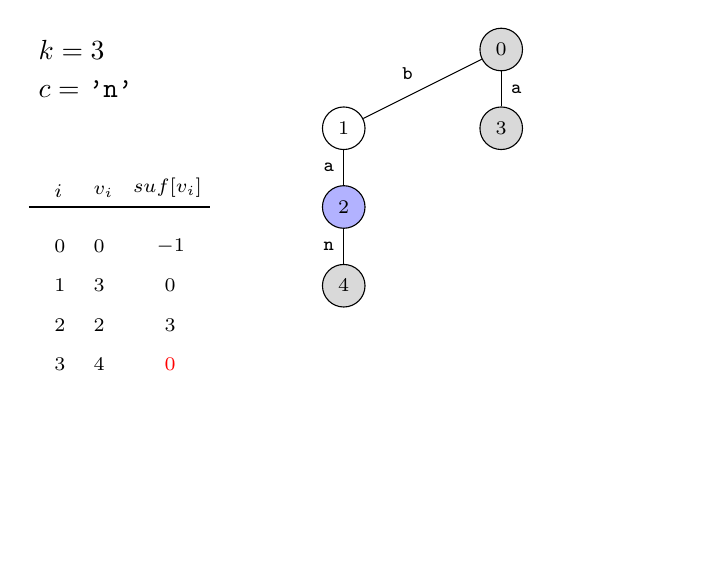
\begin{tikzpicture}
            \node[anchor=west] at (-2, 7) { $k = 3$ };
            \node[anchor=west,opacity=1] at (-2, 6.5) { $c = $ \texttt{'n'} };

            \node[anchor=south west] at (-1.8, 5) { \scriptsize $i$ };
            \node[anchor=south west] at (-1.3, 5) { \scriptsize $v_i$ };
            \node[anchor=south west] at (-0.8, 5) { \scriptsize $suf[v_i]$ };
            \draw[thick] (-2, 5) -- (0.3, 5);

            \node[anchor=west] at (-1.8, 4.5) { \scriptsize $0$ };
            \node[anchor=west] at (-1.3, 4.5) { \scriptsize $0$ };
            \node[anchor=west] at (-0.5, 4.5) { \scriptsize $-1$ };
            
            \node[anchor=west] at (-1.8, 4.0) { \scriptsize $1$ };
            \node[anchor=west] at (-1.3, 4.0) { \scriptsize \textcolor{black}{$3$} };
            \node[anchor=west] at (-0.4, 4.0) { \scriptsize $0$ };

            \node[anchor=west] at (-1.8, 3.5) { \scriptsize $2$ };
            \node[anchor=west] at (-1.3, 3.5) { \scriptsize $2$ };
            \node[anchor=west] at (-0.4, 3.5) { \scriptsize \textcolor{black}{$3$} };

            \node[anchor=west] at (-1.8, 3.0) { \scriptsize $3$ };
            \node[anchor=west] at (-1.3, 3.0) { \scriptsize $4$ };
            \node[anchor=west] at (-0.4, 3.0) { \scriptsize \textcolor{red}{$0$} };

            \node[circle,draw,opacity=1,fill=gray!30] (A) at (4, 7) {\scriptsize 0};
            \node[circle,draw,opacity=1] (B1) at (2, 6) {\scriptsize 1};
            \node[circle,draw,opacity=1,fill=gray!30] (B2) at (4, 6) {\scriptsize 3};
            \node[circle,draw,opacity=0] (B3) at (6, 6) {\scriptsize 10};
            \node[circle,draw,opacity=1,fill=blue!30] (C1) at (2, 5) {\scriptsize 2};
            \node[circle,draw,opacity=0] (C2) at (4, 5) {\scriptsize 10};
            \node[circle,draw,opacity=0] (C3) at (6, 5) {\scriptsize 10};
            \node[circle,draw,opacity=1,fill=gray!30] (D1) at (2, 4) {\scriptsize 4};
            \node[circle,draw,opacity=0] (D2) at (4, 4) {\scriptsize 10};
            \node[circle,draw,opacity=0] (D3) at (6, 4) {\scriptsize 10};
            \node[circle,draw,opacity=0] (E1) at (2, 3) {\scriptsize 10};
            \node[circle,draw,opacity=0] (E2) at (4, 3) {\scriptsize 10};
            \node[circle,draw,opacity=0] (E3) at (6, 3) {\scriptsize 10};
            \node[circle,draw,opacity=0] (F1) at (2, 2) {\scriptsize 10};
            \node[circle,draw,opacity=0] (F2) at (4, 2) {\scriptsize 10};
            \node[circle,draw,opacity=0] (G1) at (2, 1) {\scriptsize 10};

            \draw (A) -- node[anchor=south east] { \tt \scriptsize b } (B1);
            \draw (A) -- node[anchor=west] { \tt \scriptsize a } (B2);
%            \draw (A) -- node[anchor=south west] { N } (B3);
            \draw (B1) -- node[anchor=east] { \tt \scriptsize a } (C1);
%            \draw (B2) -- node[anchor=west] { N } (C2);
%            \draw (B3) -- node[anchor=west] { A } (C3);
            \draw (C1) -- node[anchor=east] { \tt \scriptsize n } (D1);
%            \draw (C2) -- node[anchor=west] { A } (D2);
%            \draw (C3) -- node[anchor=west] { N } (D3);
%            \draw (D1) -- node[anchor=east] { A } (E1);
%            \draw (D2) -- node[anchor=west] { N } (E2);
%            \draw (D3) -- node[anchor=west] { A } (E3);
%            \draw (E1) -- node[anchor=east] { N } (F1);
%            \draw (E2) -- node[anchor=west] { A } (F2);
%            \draw (F1) -- node[anchor=east] { A } (G1);
%
%            \node[circle] (N1) at (G1) { };
%            \node[circle] (N2) at (F2) { };
%            \node[circle] (N3) at (E3) { };
%            \node[circle] (N4) at (D2) { };
%            \node[circle] (N5) at (C3) { };
%            \node[circle] (N6) at (B2) { };
%
%            \draw[dashed,->] (N1) -- (N2);
%            \draw[dashed,->] (N2) -- (N3);
%            \draw[dashed,->] (N3) -- (N4);
%            \draw[dashed,->] (N4) -- (N5);
%            \draw[dashed,->] (N5) -- (N6);
    \end{tikzpicture}
\end{frame}

\begin{frame}[fragile]{Visualização da construção {\it online} da {\it trie}}

    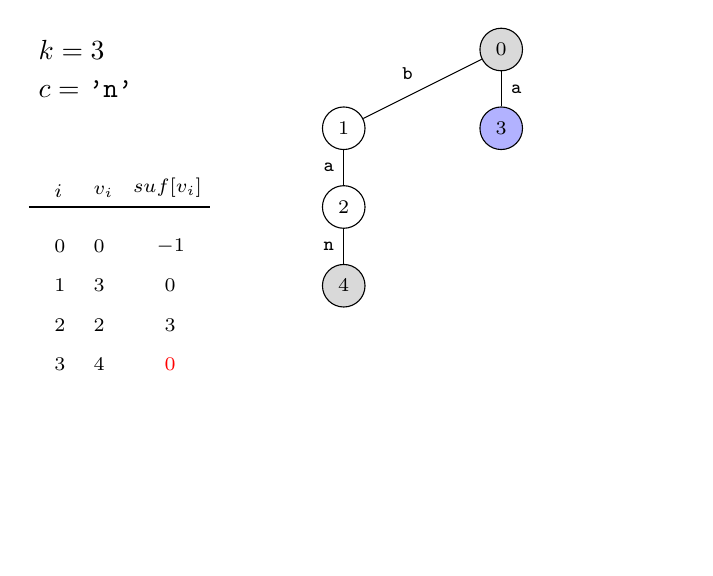
\begin{tikzpicture}
            \node[anchor=west] at (-2, 7) { $k = 3$ };
            \node[anchor=west,opacity=1] at (-2, 6.5) { $c = $ \texttt{'n'} };

            \node[anchor=south west] at (-1.8, 5) { \scriptsize $i$ };
            \node[anchor=south west] at (-1.3, 5) { \scriptsize $v_i$ };
            \node[anchor=south west] at (-0.8, 5) { \scriptsize $suf[v_i]$ };
            \draw[thick] (-2, 5) -- (0.3, 5);

            \node[anchor=west] at (-1.8, 4.5) { \scriptsize $0$ };
            \node[anchor=west] at (-1.3, 4.5) { \scriptsize $0$ };
            \node[anchor=west] at (-0.5, 4.5) { \scriptsize $-1$ };
            
            \node[anchor=west] at (-1.8, 4.0) { \scriptsize $1$ };
            \node[anchor=west] at (-1.3, 4.0) { \scriptsize \textcolor{black}{$3$} };
            \node[anchor=west] at (-0.4, 4.0) { \scriptsize $0$ };

            \node[anchor=west] at (-1.8, 3.5) { \scriptsize $2$ };
            \node[anchor=west] at (-1.3, 3.5) { \scriptsize $2$ };
            \node[anchor=west] at (-0.4, 3.5) { \scriptsize \textcolor{black}{$3$} };

            \node[anchor=west] at (-1.8, 3.0) { \scriptsize $3$ };
            \node[anchor=west] at (-1.3, 3.0) { \scriptsize $4$ };
            \node[anchor=west] at (-0.4, 3.0) { \scriptsize \textcolor{red}{$0$} };

            \node[circle,draw,opacity=1,fill=gray!30] (A) at (4, 7) {\scriptsize 0};
            \node[circle,draw,opacity=1] (B1) at (2, 6) {\scriptsize 1};
            \node[circle,draw,opacity=1,fill=blue!30] (B2) at (4, 6) {\scriptsize 3};
            \node[circle,draw,opacity=0] (B3) at (6, 6) {\scriptsize 10};
            \node[circle,draw,opacity=1] (C1) at (2, 5) {\scriptsize 2};
            \node[circle,draw,opacity=0] (C2) at (4, 5) {\scriptsize 10};
            \node[circle,draw,opacity=0] (C3) at (6, 5) {\scriptsize 10};
            \node[circle,draw,opacity=1,fill=gray!30] (D1) at (2, 4) {\scriptsize 4};
            \node[circle,draw,opacity=0] (D2) at (4, 4) {\scriptsize 10};
            \node[circle,draw,opacity=0] (D3) at (6, 4) {\scriptsize 10};
            \node[circle,draw,opacity=0] (E1) at (2, 3) {\scriptsize 10};
            \node[circle,draw,opacity=0] (E2) at (4, 3) {\scriptsize 10};
            \node[circle,draw,opacity=0] (E3) at (6, 3) {\scriptsize 10};
            \node[circle,draw,opacity=0] (F1) at (2, 2) {\scriptsize 10};
            \node[circle,draw,opacity=0] (F2) at (4, 2) {\scriptsize 10};
            \node[circle,draw,opacity=0] (G1) at (2, 1) {\scriptsize 10};

            \draw (A) -- node[anchor=south east] { \tt \scriptsize b } (B1);
            \draw (A) -- node[anchor=west] { \tt \scriptsize a } (B2);
%            \draw (A) -- node[anchor=south west] { N } (B3);
            \draw (B1) -- node[anchor=east] { \tt \scriptsize a } (C1);
%            \draw (B2) -- node[anchor=west] { N } (C2);
%            \draw (B3) -- node[anchor=west] { A } (C3);
            \draw (C1) -- node[anchor=east] { \tt \scriptsize n } (D1);
%            \draw (C2) -- node[anchor=west] { A } (D2);
%            \draw (C3) -- node[anchor=west] { N } (D3);
%            \draw (D1) -- node[anchor=east] { A } (E1);
%            \draw (D2) -- node[anchor=west] { N } (E2);
%            \draw (D3) -- node[anchor=west] { A } (E3);
%            \draw (E1) -- node[anchor=east] { N } (F1);
%            \draw (E2) -- node[anchor=west] { A } (F2);
%            \draw (F1) -- node[anchor=east] { A } (G1);
%
%            \node[circle] (N1) at (G1) { };
%            \node[circle] (N2) at (F2) { };
%            \node[circle] (N3) at (E3) { };
%            \node[circle] (N4) at (D2) { };
%            \node[circle] (N5) at (C3) { };
%            \node[circle] (N6) at (B2) { };
%
%            \draw[dashed,->] (N1) -- (N2);
%            \draw[dashed,->] (N2) -- (N3);
%            \draw[dashed,->] (N3) -- (N4);
%            \draw[dashed,->] (N4) -- (N5);
%            \draw[dashed,->] (N5) -- (N6);
    \end{tikzpicture}
\end{frame}

\begin{frame}[fragile]{Visualização da construção {\it online} da {\it trie}}

    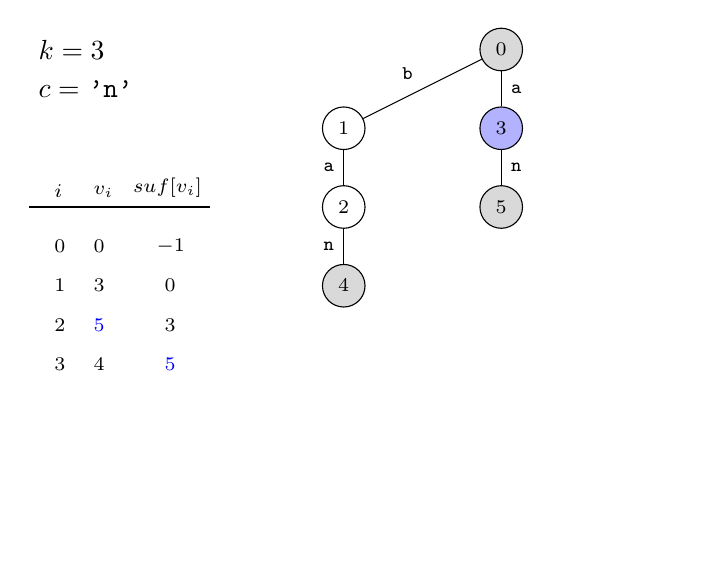
\begin{tikzpicture}
            \node[anchor=west] at (-2, 7) { $k = 3$ };
            \node[anchor=west,opacity=1] at (-2, 6.5) { $c = $ \texttt{'n'} };

            \node[anchor=south west] at (-1.8, 5) { \scriptsize $i$ };
            \node[anchor=south west] at (-1.3, 5) { \scriptsize $v_i$ };
            \node[anchor=south west] at (-0.8, 5) { \scriptsize $suf[v_i]$ };
            \draw[thick] (-2, 5) -- (0.3, 5);

            \node[anchor=west] at (-1.8, 4.5) { \scriptsize $0$ };
            \node[anchor=west] at (-1.3, 4.5) { \scriptsize $0$ };
            \node[anchor=west] at (-0.5, 4.5) { \scriptsize $-1$ };
            
            \node[anchor=west] at (-1.8, 4.0) { \scriptsize $1$ };
            \node[anchor=west] at (-1.3, 4.0) { \scriptsize \textcolor{black}{$3$} };
            \node[anchor=west] at (-0.4, 4.0) { \scriptsize $0$ };

            \node[anchor=west] at (-1.8, 3.5) { \scriptsize $2$ };
            \node[anchor=west] at (-1.3, 3.5) { \scriptsize \textcolor{blue}{$5$} };
            \node[anchor=west] at (-0.4, 3.5) { \scriptsize \textcolor{black}{$3$} };

            \node[anchor=west] at (-1.8, 3.0) { \scriptsize $3$ };
            \node[anchor=west] at (-1.3, 3.0) { \scriptsize $4$ };
            \node[anchor=west] at (-0.4, 3.0) { \scriptsize \textcolor{blue}{$5$} };

            \node[circle,draw,opacity=1,fill=gray!30] (A) at (4, 7) {\scriptsize 0};
            \node[circle,draw,opacity=1] (B1) at (2, 6) {\scriptsize 1};
            \node[circle,draw,opacity=1,fill=blue!30] (B2) at (4, 6) {\scriptsize 3};
            \node[circle,draw,opacity=0] (B3) at (6, 6) {\scriptsize 10};
            \node[circle,draw,opacity=1] (C1) at (2, 5) {\scriptsize 2};
            \node[circle,draw,opacity=1,fill=gray!30] (C2) at (4, 5) {\scriptsize 5};
            \node[circle,draw,opacity=0] (C3) at (6, 5) {\scriptsize 10};
            \node[circle,draw,opacity=1,fill=gray!30] (D1) at (2, 4) {\scriptsize 4};
            \node[circle,draw,opacity=0] (D2) at (4, 4) {\scriptsize 10};
            \node[circle,draw,opacity=0] (D3) at (6, 4) {\scriptsize 10};
            \node[circle,draw,opacity=0] (E1) at (2, 3) {\scriptsize 10};
            \node[circle,draw,opacity=0] (E2) at (4, 3) {\scriptsize 10};
            \node[circle,draw,opacity=0] (E3) at (6, 3) {\scriptsize 10};
            \node[circle,draw,opacity=0] (F1) at (2, 2) {\scriptsize 10};
            \node[circle,draw,opacity=0] (F2) at (4, 2) {\scriptsize 10};
            \node[circle,draw,opacity=0] (G1) at (2, 1) {\scriptsize 10};

            \draw (A) -- node[anchor=south east] { \tt \scriptsize b } (B1);
            \draw (A) -- node[anchor=west] { \tt \scriptsize a } (B2);
%            \draw (A) -- node[anchor=south west] { N } (B3);
            \draw (B1) -- node[anchor=east] { \tt \scriptsize a } (C1);
            \draw (B2) -- node[anchor=west] { \tt \scriptsize n } (C2);
%            \draw (B3) -- node[anchor=west] { A } (C3);
            \draw (C1) -- node[anchor=east] { \tt \scriptsize n } (D1);
%            \draw (C2) -- node[anchor=west] { A } (D2);
%            \draw (C3) -- node[anchor=west] { N } (D3);
%            \draw (D1) -- node[anchor=east] { A } (E1);
%            \draw (D2) -- node[anchor=west] { N } (E2);
%            \draw (D3) -- node[anchor=west] { A } (E3);
%            \draw (E1) -- node[anchor=east] { N } (F1);
%            \draw (E2) -- node[anchor=west] { A } (F2);
%            \draw (F1) -- node[anchor=east] { A } (G1);
%
%            \node[circle] (N1) at (G1) { };
%            \node[circle] (N2) at (F2) { };
%            \node[circle] (N3) at (E3) { };
%            \node[circle] (N4) at (D2) { };
%            \node[circle] (N5) at (C3) { };
%            \node[circle] (N6) at (B2) { };
%
%            \draw[dashed,->] (N1) -- (N2);
%            \draw[dashed,->] (N2) -- (N3);
%            \draw[dashed,->] (N3) -- (N4);
%            \draw[dashed,->] (N4) -- (N5);
%            \draw[dashed,->] (N5) -- (N6);
    \end{tikzpicture}
\end{frame}

\begin{frame}[fragile]{Visualização da construção {\it online} da {\it trie}}

    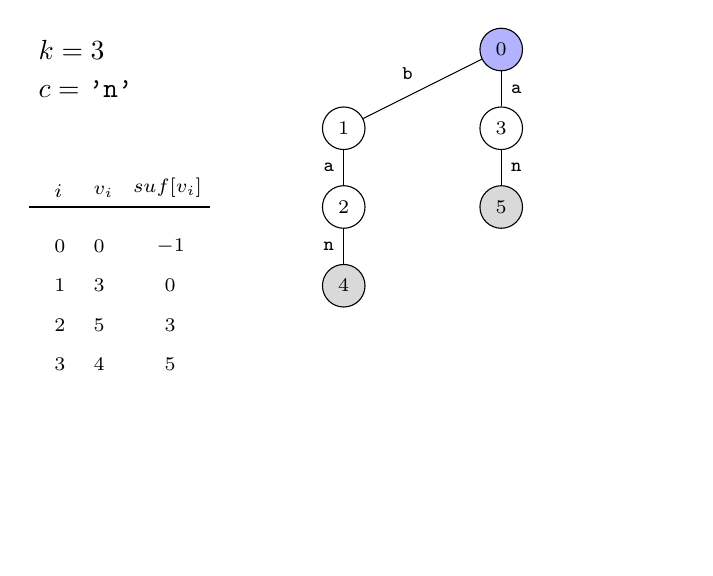
\begin{tikzpicture}
            \node[anchor=west] at (-2, 7) { $k = 3$ };
            \node[anchor=west,opacity=1] at (-2, 6.5) { $c = $ \texttt{'n'} };

            \node[anchor=south west] at (-1.8, 5) { \scriptsize $i$ };
            \node[anchor=south west] at (-1.3, 5) { \scriptsize $v_i$ };
            \node[anchor=south west] at (-0.8, 5) { \scriptsize $suf[v_i]$ };
            \draw[thick] (-2, 5) -- (0.3, 5);

            \node[anchor=west] at (-1.8, 4.5) { \scriptsize $0$ };
            \node[anchor=west] at (-1.3, 4.5) { \scriptsize $0$ };
            \node[anchor=west] at (-0.5, 4.5) { \scriptsize $-1$ };
            
            \node[anchor=west] at (-1.8, 4.0) { \scriptsize $1$ };
            \node[anchor=west] at (-1.3, 4.0) { \scriptsize \textcolor{black}{$3$} };
            \node[anchor=west] at (-0.4, 4.0) { \scriptsize $0$ };

            \node[anchor=west] at (-1.8, 3.5) { \scriptsize $2$ };
            \node[anchor=west] at (-1.3, 3.5) { \scriptsize \textcolor{black}{$5$} };
            \node[anchor=west] at (-0.4, 3.5) { \scriptsize \textcolor{black}{$3$} };

            \node[anchor=west] at (-1.8, 3.0) { \scriptsize $3$ };
            \node[anchor=west] at (-1.3, 3.0) { \scriptsize $4$ };
            \node[anchor=west] at (-0.4, 3.0) { \scriptsize \textcolor{black}{$5$} };

            \node[circle,draw,opacity=1,fill=blue!30] (A) at (4, 7) {\scriptsize 0};
            \node[circle,draw,opacity=1] (B1) at (2, 6) {\scriptsize 1};
            \node[circle,draw,opacity=1] (B2) at (4, 6) {\scriptsize 3};
            \node[circle,draw,opacity=0] (B3) at (6, 6) {\scriptsize 10};
            \node[circle,draw,opacity=1] (C1) at (2, 5) {\scriptsize 2};
            \node[circle,draw,opacity=1,fill=gray!30] (C2) at (4, 5) {\scriptsize 5};
            \node[circle,draw,opacity=0] (C3) at (6, 5) {\scriptsize 10};
            \node[circle,draw,opacity=1,fill=gray!30] (D1) at (2, 4) {\scriptsize 4};
            \node[circle,draw,opacity=0] (D2) at (4, 4) {\scriptsize 10};
            \node[circle,draw,opacity=0] (D3) at (6, 4) {\scriptsize 10};
            \node[circle,draw,opacity=0] (E1) at (2, 3) {\scriptsize 10};
            \node[circle,draw,opacity=0] (E2) at (4, 3) {\scriptsize 10};
            \node[circle,draw,opacity=0] (E3) at (6, 3) {\scriptsize 10};
            \node[circle,draw,opacity=0] (F1) at (2, 2) {\scriptsize 10};
            \node[circle,draw,opacity=0] (F2) at (4, 2) {\scriptsize 10};
            \node[circle,draw,opacity=0] (G1) at (2, 1) {\scriptsize 10};

            \draw (A) -- node[anchor=south east] { \tt \scriptsize b } (B1);
            \draw (A) -- node[anchor=west] { \tt \scriptsize a } (B2);
%            \draw (A) -- node[anchor=south west] { N } (B3);
            \draw (B1) -- node[anchor=east] { \tt \scriptsize a } (C1);
            \draw (B2) -- node[anchor=west] { \tt \scriptsize n } (C2);
%            \draw (B3) -- node[anchor=west] { A } (C3);
            \draw (C1) -- node[anchor=east] { \tt \scriptsize n } (D1);
%            \draw (C2) -- node[anchor=west] { A } (D2);
%            \draw (C3) -- node[anchor=west] { N } (D3);
%            \draw (D1) -- node[anchor=east] { A } (E1);
%            \draw (D2) -- node[anchor=west] { N } (E2);
%            \draw (D3) -- node[anchor=west] { A } (E3);
%            \draw (E1) -- node[anchor=east] { N } (F1);
%            \draw (E2) -- node[anchor=west] { A } (F2);
%            \draw (F1) -- node[anchor=east] { A } (G1);
%
%            \node[circle] (N1) at (G1) { };
%            \node[circle] (N2) at (F2) { };
%            \node[circle] (N3) at (E3) { };
%            \node[circle] (N4) at (D2) { };
%            \node[circle] (N5) at (C3) { };
%            \node[circle] (N6) at (B2) { };
%
%            \draw[dashed,->] (N1) -- (N2);
%            \draw[dashed,->] (N2) -- (N3);
%            \draw[dashed,->] (N3) -- (N4);
%            \draw[dashed,->] (N4) -- (N5);
%            \draw[dashed,->] (N5) -- (N6);
    \end{tikzpicture}
\end{frame}

\begin{frame}[fragile]{Visualização da construção {\it online} da {\it trie}}

    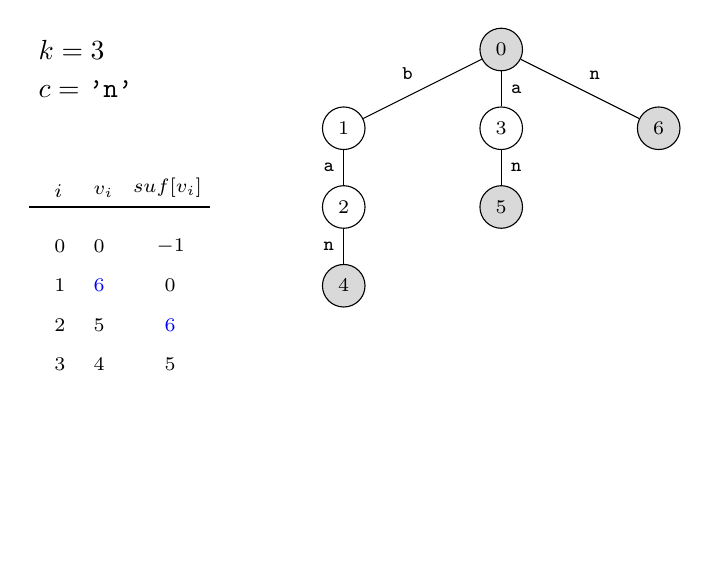
\begin{tikzpicture}
            \node[anchor=west] at (-2, 7) { $k = 3$ };
            \node[anchor=west,opacity=1] at (-2, 6.5) { $c = $ \texttt{'n'} };

            \node[anchor=south west] at (-1.8, 5) { \scriptsize $i$ };
            \node[anchor=south west] at (-1.3, 5) { \scriptsize $v_i$ };
            \node[anchor=south west] at (-0.8, 5) { \scriptsize $suf[v_i]$ };
            \draw[thick] (-2, 5) -- (0.3, 5);

            \node[anchor=west] at (-1.8, 4.5) { \scriptsize $0$ };
            \node[anchor=west] at (-1.3, 4.5) { \scriptsize $0$ };
            \node[anchor=west] at (-0.5, 4.5) { \scriptsize $-1$ };
            
            \node[anchor=west] at (-1.8, 4.0) { \scriptsize $1$ };
            \node[anchor=west] at (-1.3, 4.0) { \scriptsize \textcolor{blue}{$6$} };
            \node[anchor=west] at (-0.4, 4.0) { \scriptsize $0$ };

            \node[anchor=west] at (-1.8, 3.5) { \scriptsize $2$ };
            \node[anchor=west] at (-1.3, 3.5) { \scriptsize \textcolor{black}{$5$} };
            \node[anchor=west] at (-0.4, 3.5) { \scriptsize \textcolor{blue}{$6$} };

            \node[anchor=west] at (-1.8, 3.0) { \scriptsize $3$ };
            \node[anchor=west] at (-1.3, 3.0) { \scriptsize $4$ };
            \node[anchor=west] at (-0.4, 3.0) { \scriptsize \textcolor{black}{$5$} };

            \node[circle,draw,opacity=1,fill=gray!30] (A) at (4, 7) {\scriptsize 0};
            \node[circle,draw,opacity=1] (B1) at (2, 6) {\scriptsize 1};
            \node[circle,draw,opacity=1] (B2) at (4, 6) {\scriptsize 3};
            \node[circle,draw,opacity=1,fill=gray!30] (B3) at (6, 6) {\scriptsize 6};
            \node[circle,draw,opacity=1] (C1) at (2, 5) {\scriptsize 2};
            \node[circle,draw,opacity=1,fill=gray!30] (C2) at (4, 5) {\scriptsize 5};
            \node[circle,draw,opacity=0] (C3) at (6, 5) {\scriptsize 10};
            \node[circle,draw,opacity=1,fill=gray!30] (D1) at (2, 4) {\scriptsize 4};
            \node[circle,draw,opacity=0] (D2) at (4, 4) {\scriptsize 10};
            \node[circle,draw,opacity=0] (D3) at (6, 4) {\scriptsize 10};
            \node[circle,draw,opacity=0] (E1) at (2, 3) {\scriptsize 10};
            \node[circle,draw,opacity=0] (E2) at (4, 3) {\scriptsize 10};
            \node[circle,draw,opacity=0] (E3) at (6, 3) {\scriptsize 10};
            \node[circle,draw,opacity=0] (F1) at (2, 2) {\scriptsize 10};
            \node[circle,draw,opacity=0] (F2) at (4, 2) {\scriptsize 10};
            \node[circle,draw,opacity=0] (G1) at (2, 1) {\scriptsize 10};

            \draw (A) -- node[anchor=south east] { \tt \scriptsize b } (B1);
            \draw (A) -- node[anchor=west] { \tt \scriptsize a } (B2);
            \draw (A) -- node[anchor=south west] { \tt \scriptsize n } (B3);
            \draw (B1) -- node[anchor=east] { \tt \scriptsize a } (C1);
            \draw (B2) -- node[anchor=west] { \tt \scriptsize n } (C2);
%            \draw (B3) -- node[anchor=west] { A } (C3);
            \draw (C1) -- node[anchor=east] { \tt \scriptsize n } (D1);
%            \draw (C2) -- node[anchor=west] { A } (D2);
%            \draw (C3) -- node[anchor=west] { N } (D3);
%            \draw (D1) -- node[anchor=east] { A } (E1);
%            \draw (D2) -- node[anchor=west] { N } (E2);
%            \draw (D3) -- node[anchor=west] { A } (E3);
%            \draw (E1) -- node[anchor=east] { N } (F1);
%            \draw (E2) -- node[anchor=west] { A } (F2);
%            \draw (F1) -- node[anchor=east] { A } (G1);
%
%            \node[circle] (N1) at (G1) { };
%            \node[circle] (N2) at (F2) { };
%            \node[circle] (N3) at (E3) { };
%            \node[circle] (N4) at (D2) { };
%            \node[circle] (N5) at (C3) { };
%            \node[circle] (N6) at (B2) { };
%
%            \draw[dashed,->] (N1) -- (N2);
%            \draw[dashed,->] (N2) -- (N3);
%            \draw[dashed,->] (N3) -- (N4);
%            \draw[dashed,->] (N4) -- (N5);
%            \draw[dashed,->] (N5) -- (N6);
    \end{tikzpicture}
\end{frame}

\begin{frame}[fragile]{Visualização da construção {\it online} da {\it trie}}

    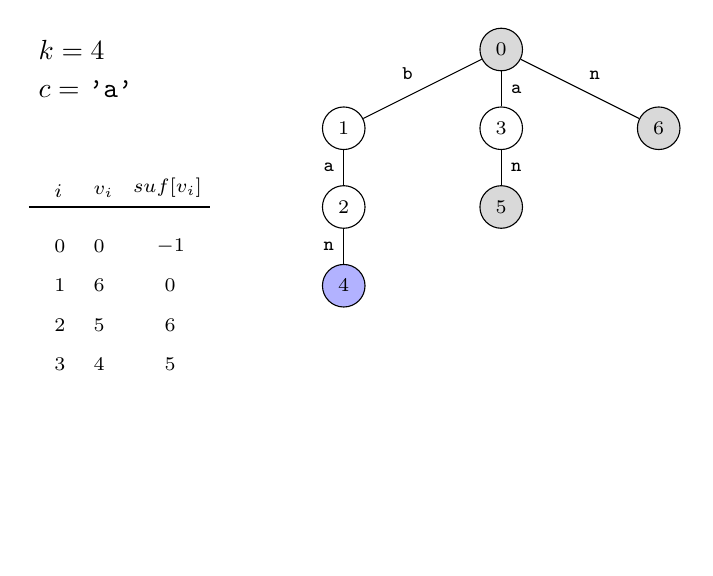
\begin{tikzpicture}
            \node[anchor=west] at (-2, 7) { $k = 4$ };
            \node[anchor=west,opacity=1] at (-2, 6.5) { $c = $ \texttt{'a'} };

            \node[anchor=south west] at (-1.8, 5) { \scriptsize $i$ };
            \node[anchor=south west] at (-1.3, 5) { \scriptsize $v_i$ };
            \node[anchor=south west] at (-0.8, 5) { \scriptsize $suf[v_i]$ };
            \draw[thick] (-2, 5) -- (0.3, 5);

            \node[anchor=west] at (-1.8, 4.5) { \scriptsize $0$ };
            \node[anchor=west] at (-1.3, 4.5) { \scriptsize $0$ };
            \node[anchor=west] at (-0.5, 4.5) { \scriptsize $-1$ };
            
            \node[anchor=west] at (-1.8, 4.0) { \scriptsize $1$ };
            \node[anchor=west] at (-1.3, 4.0) { \scriptsize \textcolor{black}{$6$} };
            \node[anchor=west] at (-0.4, 4.0) { \scriptsize $0$ };

            \node[anchor=west] at (-1.8, 3.5) { \scriptsize $2$ };
            \node[anchor=west] at (-1.3, 3.5) { \scriptsize \textcolor{black}{$5$} };
            \node[anchor=west] at (-0.4, 3.5) { \scriptsize \textcolor{black}{$6$} };

            \node[anchor=west] at (-1.8, 3.0) { \scriptsize $3$ };
            \node[anchor=west] at (-1.3, 3.0) { \scriptsize $4$ };
            \node[anchor=west] at (-0.4, 3.0) { \scriptsize \textcolor{black}{$5$} };

            \node[circle,draw,opacity=1,fill=gray!30] (A) at (4, 7) {\scriptsize 0};
            \node[circle,draw,opacity=1] (B1) at (2, 6) {\scriptsize 1};
            \node[circle,draw,opacity=1] (B2) at (4, 6) {\scriptsize 3};
            \node[circle,draw,opacity=1,fill=gray!30] (B3) at (6, 6) {\scriptsize 6};
            \node[circle,draw,opacity=1] (C1) at (2, 5) {\scriptsize 2};
            \node[circle,draw,opacity=1,fill=gray!30] (C2) at (4, 5) {\scriptsize 5};
            \node[circle,draw,opacity=0] (C3) at (6, 5) {\scriptsize 10};
            \node[circle,draw,opacity=1,fill=blue!30] (D1) at (2, 4) {\scriptsize 4};
            \node[circle,draw,opacity=0] (D2) at (4, 4) {\scriptsize 10};
            \node[circle,draw,opacity=0] (D3) at (6, 4) {\scriptsize 10};
            \node[circle,draw,opacity=0] (E1) at (2, 3) {\scriptsize 10};
            \node[circle,draw,opacity=0] (E2) at (4, 3) {\scriptsize 10};
            \node[circle,draw,opacity=0] (E3) at (6, 3) {\scriptsize 10};
            \node[circle,draw,opacity=0] (F1) at (2, 2) {\scriptsize 10};
            \node[circle,draw,opacity=0] (F2) at (4, 2) {\scriptsize 10};
            \node[circle,draw,opacity=0] (G1) at (2, 1) {\scriptsize 10};

            \draw (A) -- node[anchor=south east] { \tt \scriptsize b } (B1);
            \draw (A) -- node[anchor=west] { \tt \scriptsize a } (B2);
            \draw (A) -- node[anchor=south west] { \tt \scriptsize n } (B3);
            \draw (B1) -- node[anchor=east] { \tt \scriptsize a } (C1);
            \draw (B2) -- node[anchor=west] { \tt \scriptsize n } (C2);
%            \draw (B3) -- node[anchor=west] { A } (C3);
            \draw (C1) -- node[anchor=east] { \tt \scriptsize n } (D1);
%            \draw (C2) -- node[anchor=west] { A } (D2);
%            \draw (C3) -- node[anchor=west] { N } (D3);
%            \draw (D1) -- node[anchor=east] { A } (E1);
%            \draw (D2) -- node[anchor=west] { N } (E2);
%            \draw (D3) -- node[anchor=west] { A } (E3);
%            \draw (E1) -- node[anchor=east] { N } (F1);
%            \draw (E2) -- node[anchor=west] { A } (F2);
%            \draw (F1) -- node[anchor=east] { A } (G1);
%
%            \node[circle] (N1) at (G1) { };
%            \node[circle] (N2) at (F2) { };
%            \node[circle] (N3) at (E3) { };
%            \node[circle] (N4) at (D2) { };
%            \node[circle] (N5) at (C3) { };
%            \node[circle] (N6) at (B2) { };
%
%            \draw[dashed,->] (N1) -- (N2);
%            \draw[dashed,->] (N2) -- (N3);
%            \draw[dashed,->] (N3) -- (N4);
%            \draw[dashed,->] (N4) -- (N5);
%            \draw[dashed,->] (N5) -- (N6);
    \end{tikzpicture}
\end{frame}

\begin{frame}[fragile]{Visualização da construção {\it online} da {\it trie}}

    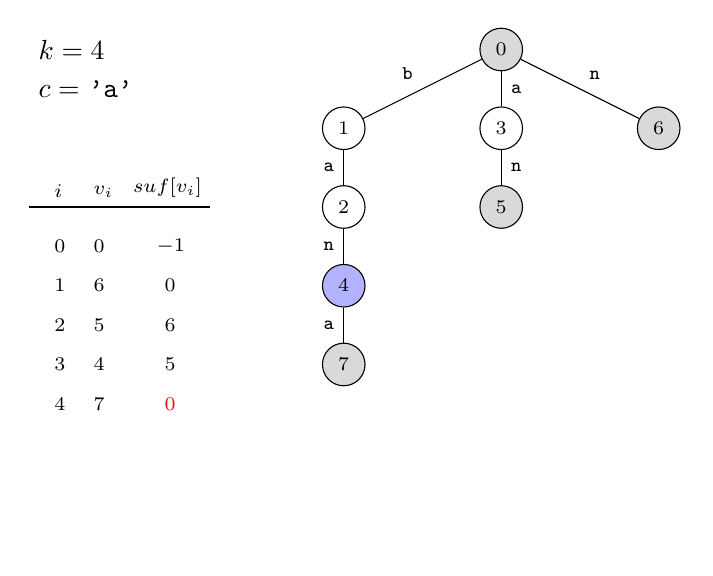
\begin{tikzpicture}
            \node[anchor=west] at (-2, 7) { $k = 4$ };
            \node[anchor=west,opacity=1] at (-2, 6.5) { $c = $ \texttt{'a'} };

            \node[anchor=south west] at (-1.8, 5) { \scriptsize $i$ };
            \node[anchor=south west] at (-1.3, 5) { \scriptsize $v_i$ };
            \node[anchor=south west] at (-0.8, 5) { \scriptsize $suf[v_i]$ };
            \draw[thick] (-2, 5) -- (0.3, 5);

            \node[anchor=west] at (-1.8, 4.5) { \scriptsize $0$ };
            \node[anchor=west] at (-1.3, 4.5) { \scriptsize $0$ };
            \node[anchor=west] at (-0.5, 4.5) { \scriptsize $-1$ };
            
            \node[anchor=west] at (-1.8, 4.0) { \scriptsize $1$ };
            \node[anchor=west] at (-1.3, 4.0) { \scriptsize \textcolor{black}{$6$} };
            \node[anchor=west] at (-0.4, 4.0) { \scriptsize $0$ };

            \node[anchor=west] at (-1.8, 3.5) { \scriptsize $2$ };
            \node[anchor=west] at (-1.3, 3.5) { \scriptsize \textcolor{black}{$5$} };
            \node[anchor=west] at (-0.4, 3.5) { \scriptsize \textcolor{black}{$6$} };

            \node[anchor=west] at (-1.8, 3.0) { \scriptsize $3$ };
            \node[anchor=west] at (-1.3, 3.0) { \scriptsize $4$ };
            \node[anchor=west] at (-0.4, 3.0) { \scriptsize \textcolor{black}{$5$} };

            \node[anchor=west] at (-1.8, 2.5) { \scriptsize $4$ };
            \node[anchor=west] at (-1.3, 2.5) { \scriptsize $7$ };
            \node[anchor=west] at (-0.4, 2.5) { \scriptsize \textcolor{red}{$0$} };

            \node[circle,draw,opacity=1,fill=gray!30] (A) at (4, 7) {\scriptsize 0};
            \node[circle,draw,opacity=1] (B1) at (2, 6) {\scriptsize 1};
            \node[circle,draw,opacity=1] (B2) at (4, 6) {\scriptsize 3};
            \node[circle,draw,opacity=1,fill=gray!30] (B3) at (6, 6) {\scriptsize 6};
            \node[circle,draw,opacity=1] (C1) at (2, 5) {\scriptsize 2};
            \node[circle,draw,opacity=1,fill=gray!30] (C2) at (4, 5) {\scriptsize 5};
            \node[circle,draw,opacity=0] (C3) at (6, 5) {\scriptsize 10};
            \node[circle,draw,opacity=1,fill=blue!30] (D1) at (2, 4) {\scriptsize 4};
            \node[circle,draw,opacity=0] (D2) at (4, 4) {\scriptsize 10};
            \node[circle,draw,opacity=0] (D3) at (6, 4) {\scriptsize 10};
            \node[circle,draw,opacity=1,fill=gray!30] (E1) at (2, 3) {\scriptsize 7};
            \node[circle,draw,opacity=0] (E2) at (4, 3) {\scriptsize 10};
            \node[circle,draw,opacity=0] (E3) at (6, 3) {\scriptsize 10};
            \node[circle,draw,opacity=0] (F1) at (2, 2) {\scriptsize 10};
            \node[circle,draw,opacity=0] (F2) at (4, 2) {\scriptsize 10};
            \node[circle,draw,opacity=0] (G1) at (2, 1) {\scriptsize 10};

            \draw (A) -- node[anchor=south east] { \tt \scriptsize b } (B1);
            \draw (A) -- node[anchor=west] { \tt \scriptsize a } (B2);
            \draw (A) -- node[anchor=south west] { \tt \scriptsize n } (B3);
            \draw (B1) -- node[anchor=east] { \tt \scriptsize a } (C1);
            \draw (B2) -- node[anchor=west] { \tt \scriptsize n } (C2);
%            \draw (B3) -- node[anchor=west] { A } (C3);
            \draw (C1) -- node[anchor=east] { \tt \scriptsize n } (D1);
%            \draw (C2) -- node[anchor=west] { A } (D2);
%            \draw (C3) -- node[anchor=west] { N } (D3);
            \draw (D1) -- node[anchor=east] { \tt \scriptsize a } (E1);
%            \draw (D2) -- node[anchor=west] { N } (E2);
%            \draw (D3) -- node[anchor=west] { A } (E3);
%            \draw (E1) -- node[anchor=east] { N } (F1);
%            \draw (E2) -- node[anchor=west] { A } (F2);
%            \draw (F1) -- node[anchor=east] { A } (G1);
%
%            \node[circle] (N1) at (G1) { };
%            \node[circle] (N2) at (F2) { };
%            \node[circle] (N3) at (E3) { };
%            \node[circle] (N4) at (D2) { };
%            \node[circle] (N5) at (C3) { };
%            \node[circle] (N6) at (B2) { };
%
%            \draw[dashed,->] (N1) -- (N2);
%            \draw[dashed,->] (N2) -- (N3);
%            \draw[dashed,->] (N3) -- (N4);
%            \draw[dashed,->] (N4) -- (N5);
%            \draw[dashed,->] (N5) -- (N6);
    \end{tikzpicture}
\end{frame}

\begin{frame}[fragile]{Visualização da construção {\it online} da {\it trie}}

    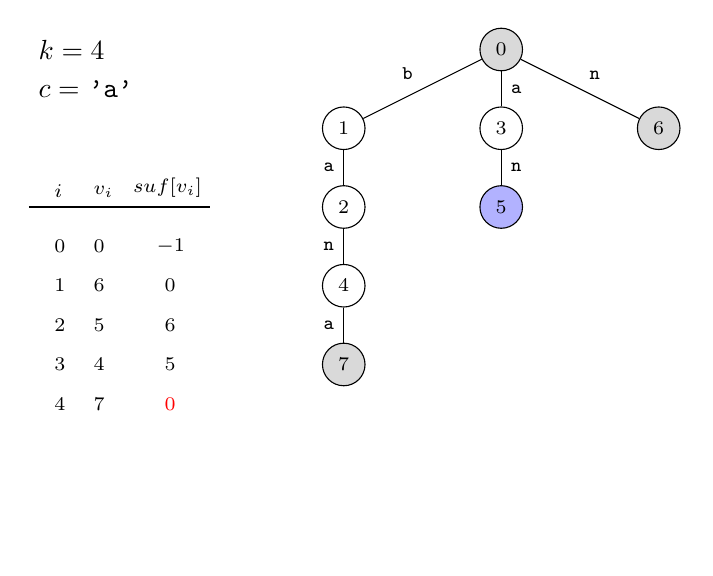
\begin{tikzpicture}
            \node[anchor=west] at (-2, 7) { $k = 4$ };
            \node[anchor=west,opacity=1] at (-2, 6.5) { $c = $ \texttt{'a'} };

            \node[anchor=south west] at (-1.8, 5) { \scriptsize $i$ };
            \node[anchor=south west] at (-1.3, 5) { \scriptsize $v_i$ };
            \node[anchor=south west] at (-0.8, 5) { \scriptsize $suf[v_i]$ };
            \draw[thick] (-2, 5) -- (0.3, 5);

            \node[anchor=west] at (-1.8, 4.5) { \scriptsize $0$ };
            \node[anchor=west] at (-1.3, 4.5) { \scriptsize $0$ };
            \node[anchor=west] at (-0.5, 4.5) { \scriptsize $-1$ };
            
            \node[anchor=west] at (-1.8, 4.0) { \scriptsize $1$ };
            \node[anchor=west] at (-1.3, 4.0) { \scriptsize \textcolor{black}{$6$} };
            \node[anchor=west] at (-0.4, 4.0) { \scriptsize $0$ };

            \node[anchor=west] at (-1.8, 3.5) { \scriptsize $2$ };
            \node[anchor=west] at (-1.3, 3.5) { \scriptsize \textcolor{black}{$5$} };
            \node[anchor=west] at (-0.4, 3.5) { \scriptsize \textcolor{black}{$6$} };

            \node[anchor=west] at (-1.8, 3.0) { \scriptsize $3$ };
            \node[anchor=west] at (-1.3, 3.0) { \scriptsize $4$ };
            \node[anchor=west] at (-0.4, 3.0) { \scriptsize \textcolor{black}{$5$} };

            \node[anchor=west] at (-1.8, 2.5) { \scriptsize $4$ };
            \node[anchor=west] at (-1.3, 2.5) { \scriptsize $7$ };
            \node[anchor=west] at (-0.4, 2.5) { \scriptsize \textcolor{red}{$0$} };

            \node[circle,draw,opacity=1,fill=gray!30] (A) at (4, 7) {\scriptsize 0};
            \node[circle,draw,opacity=1] (B1) at (2, 6) {\scriptsize 1};
            \node[circle,draw,opacity=1] (B2) at (4, 6) {\scriptsize 3};
            \node[circle,draw,opacity=1,fill=gray!30] (B3) at (6, 6) {\scriptsize 6};
            \node[circle,draw,opacity=1] (C1) at (2, 5) {\scriptsize 2};
            \node[circle,draw,opacity=1,fill=blue!30] (C2) at (4, 5) {\scriptsize 5};
            \node[circle,draw,opacity=0] (C3) at (6, 5) {\scriptsize 10};
            \node[circle,draw,opacity=1] (D1) at (2, 4) {\scriptsize 4};
            \node[circle,draw,opacity=0] (D2) at (4, 4) {\scriptsize 10};
            \node[circle,draw,opacity=0] (D3) at (6, 4) {\scriptsize 10};
            \node[circle,draw,opacity=1,fill=gray!30] (E1) at (2, 3) {\scriptsize 7};
            \node[circle,draw,opacity=0] (E2) at (4, 3) {\scriptsize 10};
            \node[circle,draw,opacity=0] (E3) at (6, 3) {\scriptsize 10};
            \node[circle,draw,opacity=0] (F1) at (2, 2) {\scriptsize 10};
            \node[circle,draw,opacity=0] (F2) at (4, 2) {\scriptsize 10};
            \node[circle,draw,opacity=0] (G1) at (2, 1) {\scriptsize 10};

            \draw (A) -- node[anchor=south east] { \tt \scriptsize b } (B1);
            \draw (A) -- node[anchor=west] { \tt \scriptsize a } (B2);
            \draw (A) -- node[anchor=south west] { \tt \scriptsize n } (B3);
            \draw (B1) -- node[anchor=east] { \tt \scriptsize a } (C1);
            \draw (B2) -- node[anchor=west] { \tt \scriptsize n } (C2);
%            \draw (B3) -- node[anchor=west] { A } (C3);
            \draw (C1) -- node[anchor=east] { \tt \scriptsize n } (D1);
%            \draw (C2) -- node[anchor=west] { A } (D2);
%            \draw (C3) -- node[anchor=west] { N } (D3);
            \draw (D1) -- node[anchor=east] { \tt \scriptsize a } (E1);
%            \draw (D2) -- node[anchor=west] { N } (E2);
%            \draw (D3) -- node[anchor=west] { A } (E3);
%            \draw (E1) -- node[anchor=east] { N } (F1);
%            \draw (E2) -- node[anchor=west] { A } (F2);
%            \draw (F1) -- node[anchor=east] { A } (G1);
%
%            \node[circle] (N1) at (G1) { };
%            \node[circle] (N2) at (F2) { };
%            \node[circle] (N3) at (E3) { };
%            \node[circle] (N4) at (D2) { };
%            \node[circle] (N5) at (C3) { };
%            \node[circle] (N6) at (B2) { };
%
%            \draw[dashed,->] (N1) -- (N2);
%            \draw[dashed,->] (N2) -- (N3);
%            \draw[dashed,->] (N3) -- (N4);
%            \draw[dashed,->] (N4) -- (N5);
%            \draw[dashed,->] (N5) -- (N6);
    \end{tikzpicture}
\end{frame}

\begin{frame}[fragile]{Visualização da construção {\it online} da {\it trie}}

    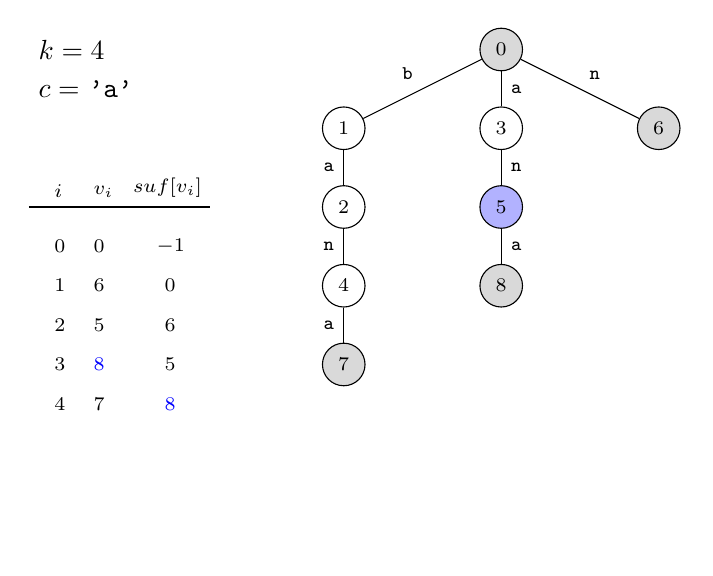
\begin{tikzpicture}
            \node[anchor=west] at (-2, 7) { $k = 4$ };
            \node[anchor=west,opacity=1] at (-2, 6.5) { $c = $ \texttt{'a'} };

            \node[anchor=south west] at (-1.8, 5) { \scriptsize $i$ };
            \node[anchor=south west] at (-1.3, 5) { \scriptsize $v_i$ };
            \node[anchor=south west] at (-0.8, 5) { \scriptsize $suf[v_i]$ };
            \draw[thick] (-2, 5) -- (0.3, 5);

            \node[anchor=west] at (-1.8, 4.5) { \scriptsize $0$ };
            \node[anchor=west] at (-1.3, 4.5) { \scriptsize $0$ };
            \node[anchor=west] at (-0.5, 4.5) { \scriptsize $-1$ };
            
            \node[anchor=west] at (-1.8, 4.0) { \scriptsize $1$ };
            \node[anchor=west] at (-1.3, 4.0) { \scriptsize \textcolor{black}{$6$} };
            \node[anchor=west] at (-0.4, 4.0) { \scriptsize $0$ };

            \node[anchor=west] at (-1.8, 3.5) { \scriptsize $2$ };
            \node[anchor=west] at (-1.3, 3.5) { \scriptsize \textcolor{black}{$5$} };
            \node[anchor=west] at (-0.4, 3.5) { \scriptsize \textcolor{black}{$6$} };

            \node[anchor=west] at (-1.8, 3.0) { \scriptsize $3$ };
            \node[anchor=west] at (-1.3, 3.0) { \scriptsize \textcolor{blue}{$8$} };
            \node[anchor=west] at (-0.4, 3.0) { \scriptsize \textcolor{black}{$5$} };

            \node[anchor=west] at (-1.8, 2.5) { \scriptsize $4$ };
            \node[anchor=west] at (-1.3, 2.5) { \scriptsize $7$ };
            \node[anchor=west] at (-0.4, 2.5) { \scriptsize \textcolor{blue}{$8$} };

            \node[circle,draw,opacity=1,fill=gray!30] (A) at (4, 7) {\scriptsize 0};
            \node[circle,draw,opacity=1] (B1) at (2, 6) {\scriptsize 1};
            \node[circle,draw,opacity=1] (B2) at (4, 6) {\scriptsize 3};
            \node[circle,draw,opacity=1,fill=gray!30] (B3) at (6, 6) {\scriptsize 6};
            \node[circle,draw,opacity=1] (C1) at (2, 5) {\scriptsize 2};
            \node[circle,draw,opacity=1,fill=blue!30] (C2) at (4, 5) {\scriptsize 5};
            \node[circle,draw,opacity=0] (C3) at (6, 5) {\scriptsize 10};
            \node[circle,draw,opacity=1] (D1) at (2, 4) {\scriptsize 4};
            \node[circle,draw,opacity=1,fill=gray!30] (D2) at (4, 4) {\scriptsize 8};
            \node[circle,draw,opacity=0] (D3) at (6, 4) {\scriptsize 10};
            \node[circle,draw,opacity=1,fill=gray!30] (E1) at (2, 3) {\scriptsize 7};
            \node[circle,draw,opacity=0] (E2) at (4, 3) {\scriptsize 10};
            \node[circle,draw,opacity=0] (E3) at (6, 3) {\scriptsize 10};
            \node[circle,draw,opacity=0] (F1) at (2, 2) {\scriptsize 10};
            \node[circle,draw,opacity=0] (F2) at (4, 2) {\scriptsize 10};
            \node[circle,draw,opacity=0] (G1) at (2, 1) {\scriptsize 10};

            \draw (A) -- node[anchor=south east] { \tt \scriptsize b } (B1);
            \draw (A) -- node[anchor=west] { \tt \scriptsize a } (B2);
            \draw (A) -- node[anchor=south west] { \tt \scriptsize n } (B3);
            \draw (B1) -- node[anchor=east] { \tt \scriptsize a } (C1);
            \draw (B2) -- node[anchor=west] { \tt \scriptsize n } (C2);
%            \draw (B3) -- node[anchor=west] { A } (C3);
            \draw (C1) -- node[anchor=east] { \tt \scriptsize n } (D1);
            \draw (C2) -- node[anchor=west] { \tt \scriptsize a } (D2);
%            \draw (C3) -- node[anchor=west] { N } (D3);
            \draw (D1) -- node[anchor=east] { \tt \scriptsize a } (E1);
%            \draw (D2) -- node[anchor=west] { N } (E2);
%            \draw (D3) -- node[anchor=west] { A } (E3);
%            \draw (E1) -- node[anchor=east] { N } (F1);
%            \draw (E2) -- node[anchor=west] { A } (F2);
%            \draw (F1) -- node[anchor=east] { A } (G1);
%
%            \node[circle] (N1) at (G1) { };
%            \node[circle] (N2) at (F2) { };
%            \node[circle] (N3) at (E3) { };
%            \node[circle] (N4) at (D2) { };
%            \node[circle] (N5) at (C3) { };
%            \node[circle] (N6) at (B2) { };
%
%            \draw[dashed,->] (N1) -- (N2);
%            \draw[dashed,->] (N2) -- (N3);
%            \draw[dashed,->] (N3) -- (N4);
%            \draw[dashed,->] (N4) -- (N5);
%            \draw[dashed,->] (N5) -- (N6);
    \end{tikzpicture}
\end{frame}

\begin{frame}[fragile]{Visualização da construção {\it online} da {\it trie}}

    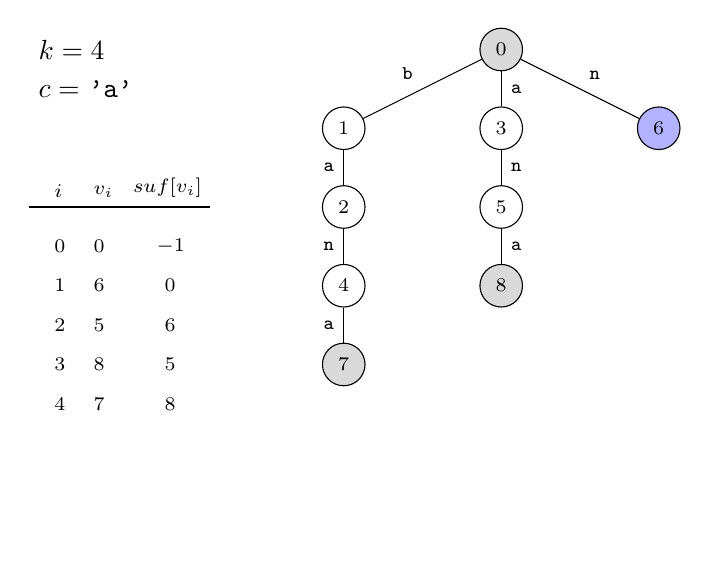
\begin{tikzpicture}
            \node[anchor=west] at (-2, 7) { $k = 4$ };
            \node[anchor=west,opacity=1] at (-2, 6.5) { $c = $ \texttt{'a'} };

            \node[anchor=south west] at (-1.8, 5) { \scriptsize $i$ };
            \node[anchor=south west] at (-1.3, 5) { \scriptsize $v_i$ };
            \node[anchor=south west] at (-0.8, 5) { \scriptsize $suf[v_i]$ };
            \draw[thick] (-2, 5) -- (0.3, 5);

            \node[anchor=west] at (-1.8, 4.5) { \scriptsize $0$ };
            \node[anchor=west] at (-1.3, 4.5) { \scriptsize $0$ };
            \node[anchor=west] at (-0.5, 4.5) { \scriptsize $-1$ };
            
            \node[anchor=west] at (-1.8, 4.0) { \scriptsize $1$ };
            \node[anchor=west] at (-1.3, 4.0) { \scriptsize \textcolor{black}{$6$} };
            \node[anchor=west] at (-0.4, 4.0) { \scriptsize $0$ };

            \node[anchor=west] at (-1.8, 3.5) { \scriptsize $2$ };
            \node[anchor=west] at (-1.3, 3.5) { \scriptsize \textcolor{black}{$5$} };
            \node[anchor=west] at (-0.4, 3.5) { \scriptsize \textcolor{black}{$6$} };

            \node[anchor=west] at (-1.8, 3.0) { \scriptsize $3$ };
            \node[anchor=west] at (-1.3, 3.0) { \scriptsize \textcolor{black}{$8$} };
            \node[anchor=west] at (-0.4, 3.0) { \scriptsize \textcolor{black}{$5$} };

            \node[anchor=west] at (-1.8, 2.5) { \scriptsize $4$ };
            \node[anchor=west] at (-1.3, 2.5) { \scriptsize $7$ };
            \node[anchor=west] at (-0.4, 2.5) { \scriptsize \textcolor{black}{$8$} };

            \node[circle,draw,opacity=1,fill=gray!30] (A) at (4, 7) {\scriptsize 0};
            \node[circle,draw,opacity=1] (B1) at (2, 6) {\scriptsize 1};
            \node[circle,draw,opacity=1] (B2) at (4, 6) {\scriptsize 3};
            \node[circle,draw,opacity=1,fill=blue!30] (B3) at (6, 6) {\scriptsize 6};
            \node[circle,draw,opacity=1] (C1) at (2, 5) {\scriptsize 2};
            \node[circle,draw,opacity=1] (C2) at (4, 5) {\scriptsize 5};
            \node[circle,draw,opacity=0] (C3) at (6, 5) {\scriptsize 10};
            \node[circle,draw,opacity=1] (D1) at (2, 4) {\scriptsize 4};
            \node[circle,draw,opacity=1,fill=gray!30] (D2) at (4, 4) {\scriptsize 8};
            \node[circle,draw,opacity=0] (D3) at (6, 4) {\scriptsize 10};
            \node[circle,draw,opacity=1,fill=gray!30] (E1) at (2, 3) {\scriptsize 7};
            \node[circle,draw,opacity=0] (E2) at (4, 3) {\scriptsize 10};
            \node[circle,draw,opacity=0] (E3) at (6, 3) {\scriptsize 10};
            \node[circle,draw,opacity=0] (F1) at (2, 2) {\scriptsize 10};
            \node[circle,draw,opacity=0] (F2) at (4, 2) {\scriptsize 10};
            \node[circle,draw,opacity=0] (G1) at (2, 1) {\scriptsize 10};

            \draw (A) -- node[anchor=south east] { \tt \scriptsize b } (B1);
            \draw (A) -- node[anchor=west] { \tt \scriptsize a } (B2);
            \draw (A) -- node[anchor=south west] { \tt \scriptsize n } (B3);
            \draw (B1) -- node[anchor=east] { \tt \scriptsize a } (C1);
            \draw (B2) -- node[anchor=west] { \tt \scriptsize n } (C2);
%            \draw (B3) -- node[anchor=west] { A } (C3);
            \draw (C1) -- node[anchor=east] { \tt \scriptsize n } (D1);
            \draw (C2) -- node[anchor=west] { \tt \scriptsize a } (D2);
%            \draw (C3) -- node[anchor=west] { N } (D3);
            \draw (D1) -- node[anchor=east] { \tt \scriptsize a } (E1);
%            \draw (D2) -- node[anchor=west] { N } (E2);
%            \draw (D3) -- node[anchor=west] { A } (E3);
%            \draw (E1) -- node[anchor=east] { N } (F1);
%            \draw (E2) -- node[anchor=west] { A } (F2);
%            \draw (F1) -- node[anchor=east] { A } (G1);
%
%            \node[circle] (N1) at (G1) { };
%            \node[circle] (N2) at (F2) { };
%            \node[circle] (N3) at (E3) { };
%            \node[circle] (N4) at (D2) { };
%            \node[circle] (N5) at (C3) { };
%            \node[circle] (N6) at (B2) { };
%
%            \draw[dashed,->] (N1) -- (N2);
%            \draw[dashed,->] (N2) -- (N3);
%            \draw[dashed,->] (N3) -- (N4);
%            \draw[dashed,->] (N4) -- (N5);
%            \draw[dashed,->] (N5) -- (N6);
    \end{tikzpicture}
\end{frame}

\begin{frame}[fragile]{Visualização da construção {\it online} da {\it trie}}

    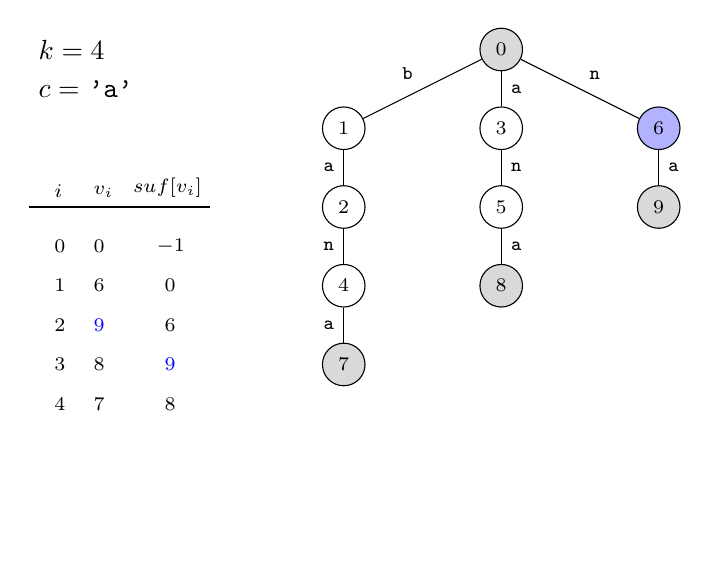
\begin{tikzpicture}
            \node[anchor=west] at (-2, 7) { $k = 4$ };
            \node[anchor=west,opacity=1] at (-2, 6.5) { $c = $ \texttt{'a'} };

            \node[anchor=south west] at (-1.8, 5) { \scriptsize $i$ };
            \node[anchor=south west] at (-1.3, 5) { \scriptsize $v_i$ };
            \node[anchor=south west] at (-0.8, 5) { \scriptsize $suf[v_i]$ };
            \draw[thick] (-2, 5) -- (0.3, 5);

            \node[anchor=west] at (-1.8, 4.5) { \scriptsize $0$ };
            \node[anchor=west] at (-1.3, 4.5) { \scriptsize $0$ };
            \node[anchor=west] at (-0.5, 4.5) { \scriptsize $-1$ };
            
            \node[anchor=west] at (-1.8, 4.0) { \scriptsize $1$ };
            \node[anchor=west] at (-1.3, 4.0) { \scriptsize \textcolor{black}{$6$} };
            \node[anchor=west] at (-0.4, 4.0) { \scriptsize $0$ };

            \node[anchor=west] at (-1.8, 3.5) { \scriptsize $2$ };
            \node[anchor=west] at (-1.3, 3.5) { \scriptsize \textcolor{blue}{$9$} };
            \node[anchor=west] at (-0.4, 3.5) { \scriptsize \textcolor{black}{$6$} };

            \node[anchor=west] at (-1.8, 3.0) { \scriptsize $3$ };
            \node[anchor=west] at (-1.3, 3.0) { \scriptsize \textcolor{black}{$8$} };
            \node[anchor=west] at (-0.4, 3.0) { \scriptsize \textcolor{blue}{$9$} };

            \node[anchor=west] at (-1.8, 2.5) { \scriptsize $4$ };
            \node[anchor=west] at (-1.3, 2.5) { \scriptsize $7$ };
            \node[anchor=west] at (-0.4, 2.5) { \scriptsize \textcolor{black}{$8$} };

            \node[circle,draw,opacity=1,fill=gray!30] (A) at (4, 7) {\scriptsize 0};
            \node[circle,draw,opacity=1] (B1) at (2, 6) {\scriptsize 1};
            \node[circle,draw,opacity=1] (B2) at (4, 6) {\scriptsize 3};
            \node[circle,draw,opacity=1,fill=blue!30] (B3) at (6, 6) {\scriptsize 6};
            \node[circle,draw,opacity=1] (C1) at (2, 5) {\scriptsize 2};
            \node[circle,draw,opacity=1] (C2) at (4, 5) {\scriptsize 5};
            \node[circle,draw,opacity=1,fill=gray!30] (C3) at (6, 5) {\scriptsize 9};
            \node[circle,draw,opacity=1] (D1) at (2, 4) {\scriptsize 4};
            \node[circle,draw,opacity=1,fill=gray!30] (D2) at (4, 4) {\scriptsize 8};
            \node[circle,draw,opacity=0] (D3) at (6, 4) {\scriptsize 10};
            \node[circle,draw,opacity=1,fill=gray!30] (E1) at (2, 3) {\scriptsize 7};
            \node[circle,draw,opacity=0] (E2) at (4, 3) {\scriptsize 10};
            \node[circle,draw,opacity=0] (E3) at (6, 3) {\scriptsize 10};
            \node[circle,draw,opacity=0] (F1) at (2, 2) {\scriptsize 10};
            \node[circle,draw,opacity=0] (F2) at (4, 2) {\scriptsize 10};
            \node[circle,draw,opacity=0] (G1) at (2, 1) {\scriptsize 10};

            \draw (A) -- node[anchor=south east] { \tt \scriptsize b } (B1);
            \draw (A) -- node[anchor=west] { \tt \scriptsize a } (B2);
            \draw (A) -- node[anchor=south west] { \tt \scriptsize n } (B3);
            \draw (B1) -- node[anchor=east] { \tt \scriptsize a } (C1);
            \draw (B2) -- node[anchor=west] { \tt \scriptsize n } (C2);
            \draw (B3) -- node[anchor=west] { \tt \scriptsize a } (C3);
            \draw (C1) -- node[anchor=east] { \tt \scriptsize n } (D1);
            \draw (C2) -- node[anchor=west] { \tt \scriptsize a } (D2);
%            \draw (C3) -- node[anchor=west] { N } (D3);
            \draw (D1) -- node[anchor=east] { \tt \scriptsize a } (E1);
%            \draw (D2) -- node[anchor=west] { N } (E2);
%            \draw (D3) -- node[anchor=west] { A } (E3);
%            \draw (E1) -- node[anchor=east] { N } (F1);
%            \draw (E2) -- node[anchor=west] { A } (F2);
%            \draw (F1) -- node[anchor=east] { A } (G1);
%
%            \node[circle] (N1) at (G1) { };
%            \node[circle] (N2) at (F2) { };
%            \node[circle] (N3) at (E3) { };
%            \node[circle] (N4) at (D2) { };
%            \node[circle] (N5) at (C3) { };
%            \node[circle] (N6) at (B2) { };
%
%            \draw[dashed,->] (N1) -- (N2);
%            \draw[dashed,->] (N2) -- (N3);
%            \draw[dashed,->] (N3) -- (N4);
%            \draw[dashed,->] (N4) -- (N5);
%            \draw[dashed,->] (N5) -- (N6);
    \end{tikzpicture}
\end{frame}

\begin{frame}[fragile]{Visualização da construção {\it online} da {\it trie}}

    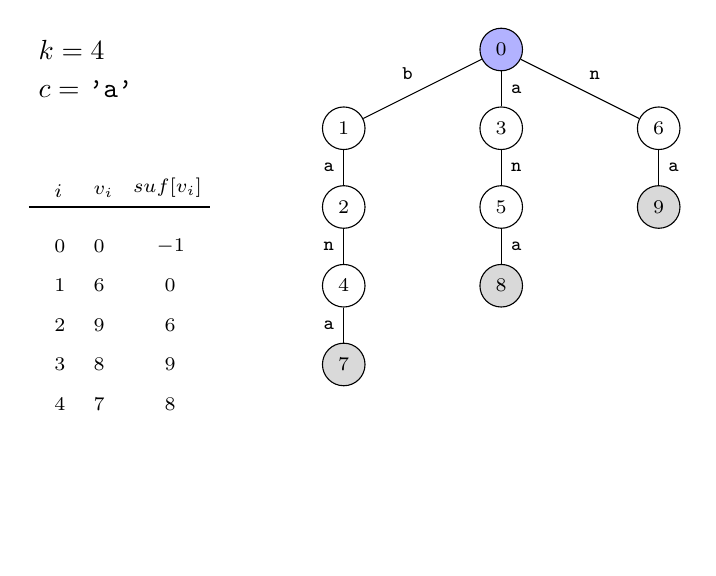
\begin{tikzpicture}
            \node[anchor=west] at (-2, 7) { $k = 4$ };
            \node[anchor=west,opacity=1] at (-2, 6.5) { $c = $ \texttt{'a'} };

            \node[anchor=south west] at (-1.8, 5) { \scriptsize $i$ };
            \node[anchor=south west] at (-1.3, 5) { \scriptsize $v_i$ };
            \node[anchor=south west] at (-0.8, 5) { \scriptsize $suf[v_i]$ };
            \draw[thick] (-2, 5) -- (0.3, 5);

            \node[anchor=west] at (-1.8, 4.5) { \scriptsize $0$ };
            \node[anchor=west] at (-1.3, 4.5) { \scriptsize $0$ };
            \node[anchor=west] at (-0.5, 4.5) { \scriptsize $-1$ };
            
            \node[anchor=west] at (-1.8, 4.0) { \scriptsize $1$ };
            \node[anchor=west] at (-1.3, 4.0) { \scriptsize \textcolor{black}{$6$} };
            \node[anchor=west] at (-0.4, 4.0) { \scriptsize $0$ };

            \node[anchor=west] at (-1.8, 3.5) { \scriptsize $2$ };
            \node[anchor=west] at (-1.3, 3.5) { \scriptsize \textcolor{black}{$9$} };
            \node[anchor=west] at (-0.4, 3.5) { \scriptsize \textcolor{black}{$6$} };

            \node[anchor=west] at (-1.8, 3.0) { \scriptsize $3$ };
            \node[anchor=west] at (-1.3, 3.0) { \scriptsize \textcolor{black}{$8$} };
            \node[anchor=west] at (-0.4, 3.0) { \scriptsize \textcolor{black}{$9$} };

            \node[anchor=west] at (-1.8, 2.5) { \scriptsize $4$ };
            \node[anchor=west] at (-1.3, 2.5) { \scriptsize $7$ };
            \node[anchor=west] at (-0.4, 2.5) { \scriptsize \textcolor{black}{$8$} };

            \node[circle,draw,opacity=1,fill=blue!30] (A) at (4, 7) {\scriptsize 0};
            \node[circle,draw,opacity=1] (B1) at (2, 6) {\scriptsize 1};
            \node[circle,draw,opacity=1] (B2) at (4, 6) {\scriptsize 3};
            \node[circle,draw,opacity=1] (B3) at (6, 6) {\scriptsize 6};
            \node[circle,draw,opacity=1] (C1) at (2, 5) {\scriptsize 2};
            \node[circle,draw,opacity=1] (C2) at (4, 5) {\scriptsize 5};
            \node[circle,draw,opacity=1,fill=gray!30] (C3) at (6, 5) {\scriptsize 9};
            \node[circle,draw,opacity=1] (D1) at (2, 4) {\scriptsize 4};
            \node[circle,draw,opacity=1,fill=gray!30] (D2) at (4, 4) {\scriptsize 8};
            \node[circle,draw,opacity=0] (D3) at (6, 4) {\scriptsize 10};
            \node[circle,draw,opacity=1,fill=gray!30] (E1) at (2, 3) {\scriptsize 7};
            \node[circle,draw,opacity=0] (E2) at (4, 3) {\scriptsize 10};
            \node[circle,draw,opacity=0] (E3) at (6, 3) {\scriptsize 10};
            \node[circle,draw,opacity=0] (F1) at (2, 2) {\scriptsize 10};
            \node[circle,draw,opacity=0] (F2) at (4, 2) {\scriptsize 10};
            \node[circle,draw,opacity=0] (G1) at (2, 1) {\scriptsize 10};

            \draw (A) -- node[anchor=south east] { \tt \scriptsize b } (B1);
            \draw (A) -- node[anchor=west] { \tt \scriptsize a } (B2);
            \draw (A) -- node[anchor=south west] { \tt \scriptsize n } (B3);
            \draw (B1) -- node[anchor=east] { \tt \scriptsize a } (C1);
            \draw (B2) -- node[anchor=west] { \tt \scriptsize n } (C2);
            \draw (B3) -- node[anchor=west] { \tt \scriptsize a } (C3);
            \draw (C1) -- node[anchor=east] { \tt \scriptsize n } (D1);
            \draw (C2) -- node[anchor=west] { \tt \scriptsize a } (D2);
%            \draw (C3) -- node[anchor=west] { N } (D3);
            \draw (D1) -- node[anchor=east] { \tt \scriptsize a } (E1);
%            \draw (D2) -- node[anchor=west] { N } (E2);
%            \draw (D3) -- node[anchor=west] { A } (E3);
%            \draw (E1) -- node[anchor=east] { N } (F1);
%            \draw (E2) -- node[anchor=west] { A } (F2);
%            \draw (F1) -- node[anchor=east] { A } (G1);
%
%            \node[circle] (N1) at (G1) { };
%            \node[circle] (N2) at (F2) { };
%            \node[circle] (N3) at (E3) { };
%            \node[circle] (N4) at (D2) { };
%            \node[circle] (N5) at (C3) { };
%            \node[circle] (N6) at (B2) { };
%
%            \draw[dashed,->] (N1) -- (N2);
%            \draw[dashed,->] (N2) -- (N3);
%            \draw[dashed,->] (N3) -- (N4);
%            \draw[dashed,->] (N4) -- (N5);
%            \draw[dashed,->] (N5) -- (N6);
    \end{tikzpicture}
\end{frame}

\begin{frame}[fragile]{Visualização da construção {\it online} da {\it trie}}

    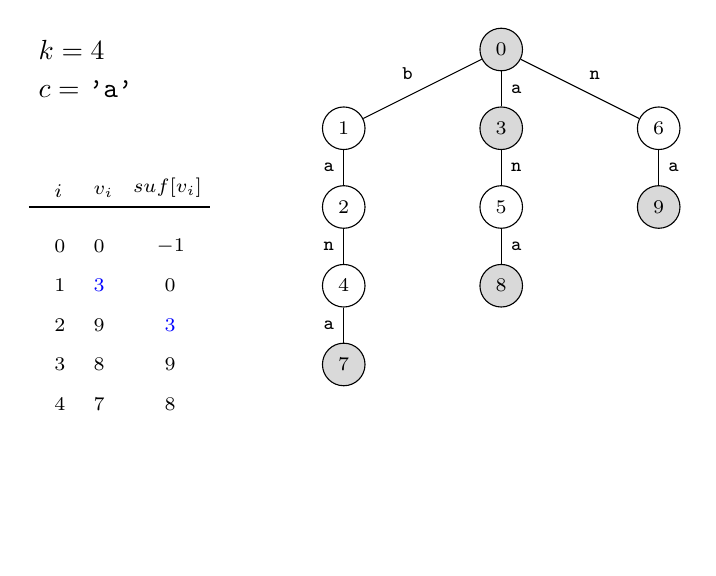
\begin{tikzpicture}
            \node[anchor=west] at (-2, 7) { $k = 4$ };
            \node[anchor=west,opacity=1] at (-2, 6.5) { $c = $ \texttt{'a'} };

            \node[anchor=south west] at (-1.8, 5) { \scriptsize $i$ };
            \node[anchor=south west] at (-1.3, 5) { \scriptsize $v_i$ };
            \node[anchor=south west] at (-0.8, 5) { \scriptsize $suf[v_i]$ };
            \draw[thick] (-2, 5) -- (0.3, 5);

            \node[anchor=west] at (-1.8, 4.5) { \scriptsize $0$ };
            \node[anchor=west] at (-1.3, 4.5) { \scriptsize $0$ };
            \node[anchor=west] at (-0.5, 4.5) { \scriptsize $-1$ };
            
            \node[anchor=west] at (-1.8, 4.0) { \scriptsize $1$ };
            \node[anchor=west] at (-1.3, 4.0) { \scriptsize \textcolor{blue}{$3$} };
            \node[anchor=west] at (-0.4, 4.0) { \scriptsize $0$ };

            \node[anchor=west] at (-1.8, 3.5) { \scriptsize $2$ };
            \node[anchor=west] at (-1.3, 3.5) { \scriptsize \textcolor{black}{$9$} };
            \node[anchor=west] at (-0.4, 3.5) { \scriptsize \textcolor{blue}{$3$} };

            \node[anchor=west] at (-1.8, 3.0) { \scriptsize $3$ };
            \node[anchor=west] at (-1.3, 3.0) { \scriptsize \textcolor{black}{$8$} };
            \node[anchor=west] at (-0.4, 3.0) { \scriptsize \textcolor{black}{$9$} };

            \node[anchor=west] at (-1.8, 2.5) { \scriptsize $4$ };
            \node[anchor=west] at (-1.3, 2.5) { \scriptsize $7$ };
            \node[anchor=west] at (-0.4, 2.5) { \scriptsize \textcolor{black}{$8$} };

            \node[circle,draw,opacity=1,fill=gray!30] (A) at (4, 7) {\scriptsize 0};
            \node[circle,draw,opacity=1] (B1) at (2, 6) {\scriptsize 1};
            \node[circle,draw,opacity=1,fill=gray!30] (B2) at (4, 6) {\scriptsize 3};
            \node[circle,draw,opacity=1] (B3) at (6, 6) {\scriptsize 6};
            \node[circle,draw,opacity=1] (C1) at (2, 5) {\scriptsize 2};
            \node[circle,draw,opacity=1] (C2) at (4, 5) {\scriptsize 5};
            \node[circle,draw,opacity=1,fill=gray!30] (C3) at (6, 5) {\scriptsize 9};
            \node[circle,draw,opacity=1] (D1) at (2, 4) {\scriptsize 4};
            \node[circle,draw,opacity=1,fill=gray!30] (D2) at (4, 4) {\scriptsize 8};
            \node[circle,draw,opacity=0] (D3) at (6, 4) {\scriptsize 10};
            \node[circle,draw,opacity=1,fill=gray!30] (E1) at (2, 3) {\scriptsize 7};
            \node[circle,draw,opacity=0] (E2) at (4, 3) {\scriptsize 10};
            \node[circle,draw,opacity=0] (E3) at (6, 3) {\scriptsize 10};
            \node[circle,draw,opacity=0] (F1) at (2, 2) {\scriptsize 10};
            \node[circle,draw,opacity=0] (F2) at (4, 2) {\scriptsize 10};
            \node[circle,draw,opacity=0] (G1) at (2, 1) {\scriptsize 10};

            \draw (A) -- node[anchor=south east] { \tt \scriptsize b } (B1);
            \draw (A) -- node[anchor=west] { \tt \scriptsize a } (B2);
            \draw (A) -- node[anchor=south west] { \tt \scriptsize n } (B3);
            \draw (B1) -- node[anchor=east] { \tt \scriptsize a } (C1);
            \draw (B2) -- node[anchor=west] { \tt \scriptsize n } (C2);
            \draw (B3) -- node[anchor=west] { \tt \scriptsize a } (C3);
            \draw (C1) -- node[anchor=east] { \tt \scriptsize n } (D1);
            \draw (C2) -- node[anchor=west] { \tt \scriptsize a } (D2);
%            \draw (C3) -- node[anchor=west] { N } (D3);
            \draw (D1) -- node[anchor=east] { \tt \scriptsize a } (E1);
%            \draw (D2) -- node[anchor=west] { N } (E2);
%            \draw (D3) -- node[anchor=west] { A } (E3);
%            \draw (E1) -- node[anchor=east] { N } (F1);
%            \draw (E2) -- node[anchor=west] { A } (F2);
%            \draw (F1) -- node[anchor=east] { A } (G1);
%
%            \node[circle] (N1) at (G1) { };
%            \node[circle] (N2) at (F2) { };
%            \node[circle] (N3) at (E3) { };
%            \node[circle] (N4) at (D2) { };
%            \node[circle] (N5) at (C3) { };
%            \node[circle] (N6) at (B2) { };
%
%            \draw[dashed,->] (N1) -- (N2);
%            \draw[dashed,->] (N2) -- (N3);
%            \draw[dashed,->] (N3) -- (N4);
%            \draw[dashed,->] (N4) -- (N5);
%            \draw[dashed,->] (N5) -- (N6);
    \end{tikzpicture}
\end{frame}

\begin{frame}[fragile]{Visualização da construção {\it online} da {\it trie}}

    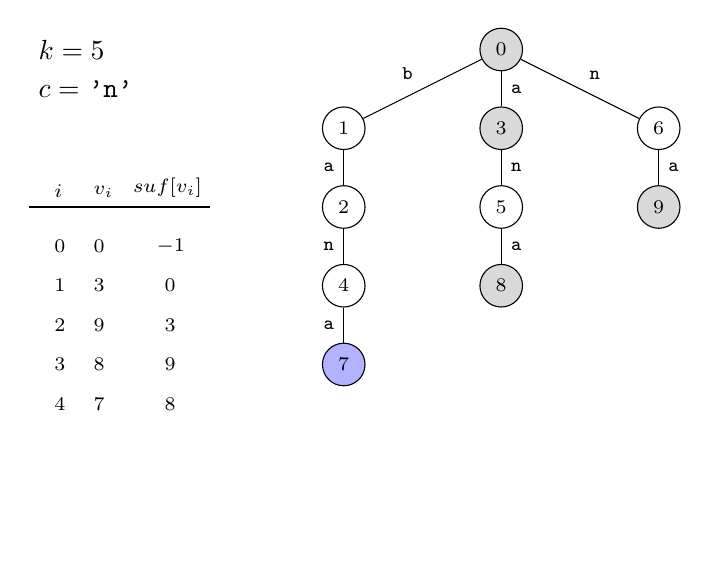
\begin{tikzpicture}
            \node[anchor=west] at (-2, 7) { $k = 5$ };
            \node[anchor=west,opacity=1] at (-2, 6.5) { $c = $ \texttt{'n'} };

            \node[anchor=south west] at (-1.8, 5) { \scriptsize $i$ };
            \node[anchor=south west] at (-1.3, 5) { \scriptsize $v_i$ };
            \node[anchor=south west] at (-0.8, 5) { \scriptsize $suf[v_i]$ };
            \draw[thick] (-2, 5) -- (0.3, 5);

            \node[anchor=west] at (-1.8, 4.5) { \scriptsize $0$ };
            \node[anchor=west] at (-1.3, 4.5) { \scriptsize $0$ };
            \node[anchor=west] at (-0.5, 4.5) { \scriptsize $-1$ };
            
            \node[anchor=west] at (-1.8, 4.0) { \scriptsize $1$ };
            \node[anchor=west] at (-1.3, 4.0) { \scriptsize \textcolor{black}{$3$} };
            \node[anchor=west] at (-0.4, 4.0) { \scriptsize $0$ };

            \node[anchor=west] at (-1.8, 3.5) { \scriptsize $2$ };
            \node[anchor=west] at (-1.3, 3.5) { \scriptsize \textcolor{black}{$9$} };
            \node[anchor=west] at (-0.4, 3.5) { \scriptsize \textcolor{black}{$3$} };

            \node[anchor=west] at (-1.8, 3.0) { \scriptsize $3$ };
            \node[anchor=west] at (-1.3, 3.0) { \scriptsize \textcolor{black}{$8$} };
            \node[anchor=west] at (-0.4, 3.0) { \scriptsize \textcolor{black}{$9$} };

            \node[anchor=west] at (-1.8, 2.5) { \scriptsize $4$ };
            \node[anchor=west] at (-1.3, 2.5) { \scriptsize $7$ };
            \node[anchor=west] at (-0.4, 2.5) { \scriptsize \textcolor{black}{$8$} };

            \node[circle,draw,opacity=1,fill=gray!30] (A) at (4, 7) {\scriptsize 0};
            \node[circle,draw,opacity=1] (B1) at (2, 6) {\scriptsize 1};
            \node[circle,draw,opacity=1,fill=gray!30] (B2) at (4, 6) {\scriptsize 3};
            \node[circle,draw,opacity=1] (B3) at (6, 6) {\scriptsize 6};
            \node[circle,draw,opacity=1] (C1) at (2, 5) {\scriptsize 2};
            \node[circle,draw,opacity=1] (C2) at (4, 5) {\scriptsize 5};
            \node[circle,draw,opacity=1,fill=gray!30] (C3) at (6, 5) {\scriptsize 9};
            \node[circle,draw,opacity=1] (D1) at (2, 4) {\scriptsize 4};
            \node[circle,draw,opacity=1,fill=gray!30] (D2) at (4, 4) {\scriptsize 8};
            \node[circle,draw,opacity=0] (D3) at (6, 4) {\scriptsize 10};
            \node[circle,draw,opacity=1,fill=blue!30] (E1) at (2, 3) {\scriptsize 7};
            \node[circle,draw,opacity=0] (E2) at (4, 3) {\scriptsize 10};
            \node[circle,draw,opacity=0] (E3) at (6, 3) {\scriptsize 10};
            \node[circle,draw,opacity=0] (F1) at (2, 2) {\scriptsize 10};
            \node[circle,draw,opacity=0] (F2) at (4, 2) {\scriptsize 10};
            \node[circle,draw,opacity=0] (G1) at (2, 1) {\scriptsize 10};

            \draw (A) -- node[anchor=south east] { \tt \scriptsize b } (B1);
            \draw (A) -- node[anchor=west] { \tt \scriptsize a } (B2);
            \draw (A) -- node[anchor=south west] { \tt \scriptsize n } (B3);
            \draw (B1) -- node[anchor=east] { \tt \scriptsize a } (C1);
            \draw (B2) -- node[anchor=west] { \tt \scriptsize n } (C2);
            \draw (B3) -- node[anchor=west] { \tt \scriptsize a } (C3);
            \draw (C1) -- node[anchor=east] { \tt \scriptsize n } (D1);
            \draw (C2) -- node[anchor=west] { \tt \scriptsize a } (D2);
%            \draw (C3) -- node[anchor=west] { N } (D3);
            \draw (D1) -- node[anchor=east] { \tt \scriptsize a } (E1);
%            \draw (D2) -- node[anchor=west] { N } (E2);
%            \draw (D3) -- node[anchor=west] { A } (E3);
%            \draw (E1) -- node[anchor=east] { N } (F1);
%            \draw (E2) -- node[anchor=west] { A } (F2);
%            \draw (F1) -- node[anchor=east] { A } (G1);
%
%            \node[circle] (N1) at (G1) { };
%            \node[circle] (N2) at (F2) { };
%            \node[circle] (N3) at (E3) { };
%            \node[circle] (N4) at (D2) { };
%            \node[circle] (N5) at (C3) { };
%            \node[circle] (N6) at (B2) { };
%
%            \draw[dashed,->] (N1) -- (N2);
%            \draw[dashed,->] (N2) -- (N3);
%            \draw[dashed,->] (N3) -- (N4);
%            \draw[dashed,->] (N4) -- (N5);
%            \draw[dashed,->] (N5) -- (N6);
    \end{tikzpicture}
\end{frame}

\begin{frame}[fragile]{Visualização da construção {\it online} da {\it trie}}

    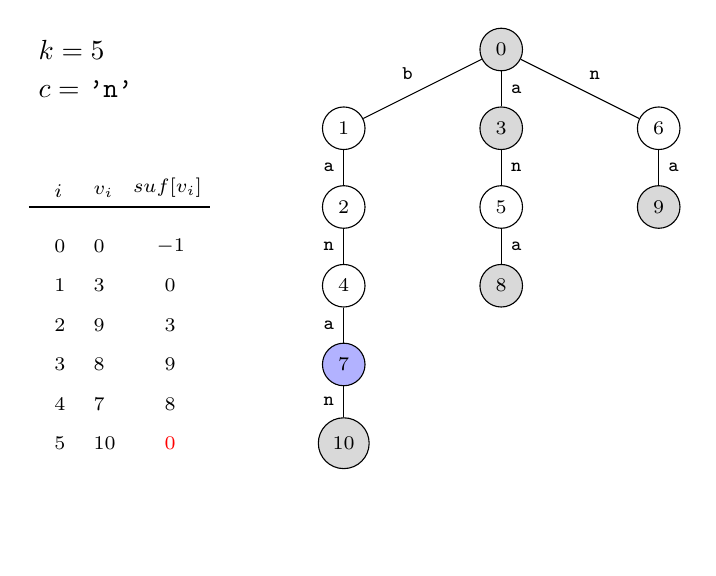
\begin{tikzpicture}
            \node[anchor=west] at (-2, 7) { $k = 5$ };
            \node[anchor=west,opacity=1] at (-2, 6.5) { $c = $ \texttt{'n'} };

            \node[anchor=south west] at (-1.8, 5) { \scriptsize $i$ };
            \node[anchor=south west] at (-1.3, 5) { \scriptsize $v_i$ };
            \node[anchor=south west] at (-0.8, 5) { \scriptsize $suf[v_i]$ };
            \draw[thick] (-2, 5) -- (0.3, 5);

            \node[anchor=west] at (-1.8, 4.5) { \scriptsize $0$ };
            \node[anchor=west] at (-1.3, 4.5) { \scriptsize $0$ };
            \node[anchor=west] at (-0.5, 4.5) { \scriptsize $-1$ };
            
            \node[anchor=west] at (-1.8, 4.0) { \scriptsize $1$ };
            \node[anchor=west] at (-1.3, 4.0) { \scriptsize \textcolor{black}{$3$} };
            \node[anchor=west] at (-0.4, 4.0) { \scriptsize $0$ };

            \node[anchor=west] at (-1.8, 3.5) { \scriptsize $2$ };
            \node[anchor=west] at (-1.3, 3.5) { \scriptsize \textcolor{black}{$9$} };
            \node[anchor=west] at (-0.4, 3.5) { \scriptsize \textcolor{black}{$3$} };

            \node[anchor=west] at (-1.8, 3.0) { \scriptsize $3$ };
            \node[anchor=west] at (-1.3, 3.0) { \scriptsize \textcolor{black}{$8$} };
            \node[anchor=west] at (-0.4, 3.0) { \scriptsize \textcolor{black}{$9$} };

            \node[anchor=west] at (-1.8, 2.5) { \scriptsize $4$ };
            \node[anchor=west] at (-1.3, 2.5) { \scriptsize $7$ };
            \node[anchor=west] at (-0.4, 2.5) { \scriptsize \textcolor{black}{$8$} };

            \node[anchor=west] at (-1.8, 2.0) { \scriptsize $5$ };
            \node[anchor=west] at (-1.3, 2.0) { \scriptsize $10$ };
            \node[anchor=west] at (-0.4, 2.0) { \scriptsize \textcolor{red}{$0$} };

            \node[circle,draw,opacity=1,fill=gray!30] (A) at (4, 7) {\scriptsize 0};
            \node[circle,draw,opacity=1] (B1) at (2, 6) {\scriptsize 1};
            \node[circle,draw,opacity=1,fill=gray!30] (B2) at (4, 6) {\scriptsize 3};
            \node[circle,draw,opacity=1] (B3) at (6, 6) {\scriptsize 6};
            \node[circle,draw,opacity=1] (C1) at (2, 5) {\scriptsize 2};
            \node[circle,draw,opacity=1] (C2) at (4, 5) {\scriptsize 5};
            \node[circle,draw,opacity=1,fill=gray!30] (C3) at (6, 5) {\scriptsize 9};
            \node[circle,draw,opacity=1] (D1) at (2, 4) {\scriptsize 4};
            \node[circle,draw,opacity=1,fill=gray!30] (D2) at (4, 4) {\scriptsize 8};
            \node[circle,draw,opacity=0] (D3) at (6, 4) {\scriptsize 10};
            \node[circle,draw,opacity=1,fill=blue!30] (E1) at (2, 3) {\scriptsize 7};
            \node[circle,draw,opacity=0] (E2) at (4, 3) {\scriptsize 10};
            \node[circle,draw,opacity=0] (E3) at (6, 3) {\scriptsize 10};
            \node[circle,draw,opacity=1,fill=gray!30] (F1) at (2, 2) {\scriptsize 10};
            \node[circle,draw,opacity=0] (F2) at (4, 2) {\scriptsize 10};
            \node[circle,draw,opacity=0] (G1) at (2, 1) {\scriptsize 10};

            \draw (A) -- node[anchor=south east] { \tt \scriptsize b } (B1);
            \draw (A) -- node[anchor=west] { \tt \scriptsize a } (B2);
            \draw (A) -- node[anchor=south west] { \tt \scriptsize n } (B3);
            \draw (B1) -- node[anchor=east] { \tt \scriptsize a } (C1);
            \draw (B2) -- node[anchor=west] { \tt \scriptsize n } (C2);
            \draw (B3) -- node[anchor=west] { \tt \scriptsize a } (C3);
            \draw (C1) -- node[anchor=east] { \tt \scriptsize n } (D1);
            \draw (C2) -- node[anchor=west] { \tt \scriptsize a } (D2);
%            \draw (C3) -- node[anchor=west] { N } (D3);
            \draw (D1) -- node[anchor=east] { \tt \scriptsize a } (E1);
%            \draw (D2) -- node[anchor=west] { N } (E2);
%            \draw (D3) -- node[anchor=west] { A } (E3);
            \draw (E1) -- node[anchor=east] { \tt \scriptsize n } (F1);
%            \draw (E2) -- node[anchor=west] { A } (F2);
%            \draw (F1) -- node[anchor=east] { A } (G1);
%
%            \node[circle] (N1) at (G1) { };
%            \node[circle] (N2) at (F2) { };
%            \node[circle] (N3) at (E3) { };
%            \node[circle] (N4) at (D2) { };
%            \node[circle] (N5) at (C3) { };
%            \node[circle] (N6) at (B2) { };
%
%            \draw[dashed,->] (N1) -- (N2);
%            \draw[dashed,->] (N2) -- (N3);
%            \draw[dashed,->] (N3) -- (N4);
%            \draw[dashed,->] (N4) -- (N5);
%            \draw[dashed,->] (N5) -- (N6);
    \end{tikzpicture}
\end{frame}

\begin{frame}[fragile]{Visualização da construção {\it online} da {\it trie}}

    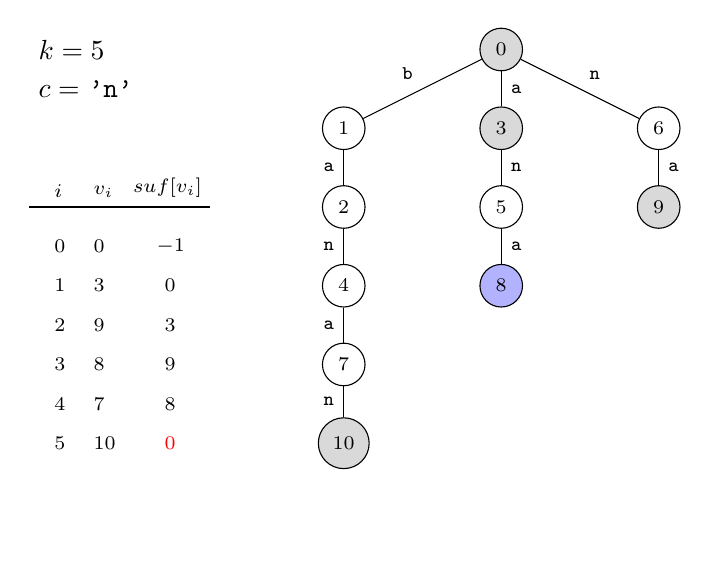
\begin{tikzpicture}
            \node[anchor=west] at (-2, 7) { $k = 5$ };
            \node[anchor=west,opacity=1] at (-2, 6.5) { $c = $ \texttt{'n'} };

            \node[anchor=south west] at (-1.8, 5) { \scriptsize $i$ };
            \node[anchor=south west] at (-1.3, 5) { \scriptsize $v_i$ };
            \node[anchor=south west] at (-0.8, 5) { \scriptsize $suf[v_i]$ };
            \draw[thick] (-2, 5) -- (0.3, 5);

            \node[anchor=west] at (-1.8, 4.5) { \scriptsize $0$ };
            \node[anchor=west] at (-1.3, 4.5) { \scriptsize $0$ };
            \node[anchor=west] at (-0.5, 4.5) { \scriptsize $-1$ };
            
            \node[anchor=west] at (-1.8, 4.0) { \scriptsize $1$ };
            \node[anchor=west] at (-1.3, 4.0) { \scriptsize \textcolor{black}{$3$} };
            \node[anchor=west] at (-0.4, 4.0) { \scriptsize $0$ };

            \node[anchor=west] at (-1.8, 3.5) { \scriptsize $2$ };
            \node[anchor=west] at (-1.3, 3.5) { \scriptsize \textcolor{black}{$9$} };
            \node[anchor=west] at (-0.4, 3.5) { \scriptsize \textcolor{black}{$3$} };

            \node[anchor=west] at (-1.8, 3.0) { \scriptsize $3$ };
            \node[anchor=west] at (-1.3, 3.0) { \scriptsize \textcolor{black}{$8$} };
            \node[anchor=west] at (-0.4, 3.0) { \scriptsize \textcolor{black}{$9$} };

            \node[anchor=west] at (-1.8, 2.5) { \scriptsize $4$ };
            \node[anchor=west] at (-1.3, 2.5) { \scriptsize $7$ };
            \node[anchor=west] at (-0.4, 2.5) { \scriptsize \textcolor{black}{$8$} };

            \node[anchor=west] at (-1.8, 2.0) { \scriptsize $5$ };
            \node[anchor=west] at (-1.3, 2.0) { \scriptsize $10$ };
            \node[anchor=west] at (-0.4, 2.0) { \scriptsize \textcolor{red}{$0$} };

            \node[circle,draw,opacity=1,fill=gray!30] (A) at (4, 7) {\scriptsize 0};
            \node[circle,draw,opacity=1] (B1) at (2, 6) {\scriptsize 1};
            \node[circle,draw,opacity=1,fill=gray!30] (B2) at (4, 6) {\scriptsize 3};
            \node[circle,draw,opacity=1] (B3) at (6, 6) {\scriptsize 6};
            \node[circle,draw,opacity=1] (C1) at (2, 5) {\scriptsize 2};
            \node[circle,draw,opacity=1] (C2) at (4, 5) {\scriptsize 5};
            \node[circle,draw,opacity=1,fill=gray!30] (C3) at (6, 5) {\scriptsize 9};
            \node[circle,draw,opacity=1] (D1) at (2, 4) {\scriptsize 4};
            \node[circle,draw,opacity=1,fill=blue!30] (D2) at (4, 4) {\scriptsize 8};
            \node[circle,draw,opacity=0] (D3) at (6, 4) {\scriptsize 10};
            \node[circle,draw,opacity=1] (E1) at (2, 3) {\scriptsize 7};
            \node[circle,draw,opacity=0] (E2) at (4, 3) {\scriptsize 10};
            \node[circle,draw,opacity=0] (E3) at (6, 3) {\scriptsize 10};
            \node[circle,draw,opacity=1,fill=gray!30] (F1) at (2, 2) {\scriptsize 10};
            \node[circle,draw,opacity=0] (F2) at (4, 2) {\scriptsize 10};
            \node[circle,draw,opacity=0] (G1) at (2, 1) {\scriptsize 10};

            \draw (A) -- node[anchor=south east] { \tt \scriptsize b } (B1);
            \draw (A) -- node[anchor=west] { \tt \scriptsize a } (B2);
            \draw (A) -- node[anchor=south west] { \tt \scriptsize n } (B3);
            \draw (B1) -- node[anchor=east] { \tt \scriptsize a } (C1);
            \draw (B2) -- node[anchor=west] { \tt \scriptsize n } (C2);
            \draw (B3) -- node[anchor=west] { \tt \scriptsize a } (C3);
            \draw (C1) -- node[anchor=east] { \tt \scriptsize n } (D1);
            \draw (C2) -- node[anchor=west] { \tt \scriptsize a } (D2);
%            \draw (C3) -- node[anchor=west] { N } (D3);
            \draw (D1) -- node[anchor=east] { \tt \scriptsize a } (E1);
%            \draw (D2) -- node[anchor=west] { N } (E2);
%            \draw (D3) -- node[anchor=west] { A } (E3);
            \draw (E1) -- node[anchor=east] { \tt \scriptsize n } (F1);
%            \draw (E2) -- node[anchor=west] { A } (F2);
%            \draw (F1) -- node[anchor=east] { A } (G1);
%
%            \node[circle] (N1) at (G1) { };
%            \node[circle] (N2) at (F2) { };
%            \node[circle] (N3) at (E3) { };
%            \node[circle] (N4) at (D2) { };
%            \node[circle] (N5) at (C3) { };
%            \node[circle] (N6) at (B2) { };
%
%            \draw[dashed,->] (N1) -- (N2);
%            \draw[dashed,->] (N2) -- (N3);
%            \draw[dashed,->] (N3) -- (N4);
%            \draw[dashed,->] (N4) -- (N5);
%            \draw[dashed,->] (N5) -- (N6);
    \end{tikzpicture}
\end{frame}

\begin{frame}[fragile]{Visualização da construção {\it online} da {\it trie}}

    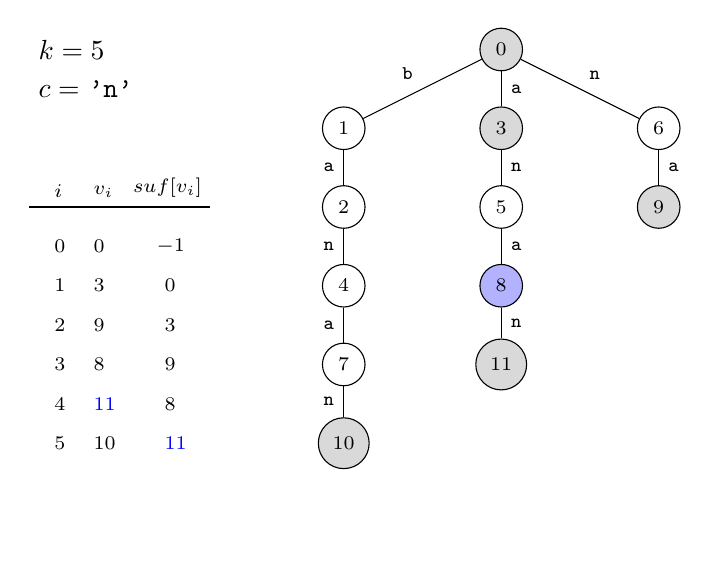
\begin{tikzpicture}
            \node[anchor=west] at (-2, 7) { $k = 5$ };
            \node[anchor=west,opacity=1] at (-2, 6.5) { $c = $ \texttt{'n'} };

            \node[anchor=south west] at (-1.8, 5) { \scriptsize $i$ };
            \node[anchor=south west] at (-1.3, 5) { \scriptsize $v_i$ };
            \node[anchor=south west] at (-0.8, 5) { \scriptsize $suf[v_i]$ };
            \draw[thick] (-2, 5) -- (0.3, 5);

            \node[anchor=west] at (-1.8, 4.5) { \scriptsize $0$ };
            \node[anchor=west] at (-1.3, 4.5) { \scriptsize $0$ };
            \node[anchor=west] at (-0.5, 4.5) { \scriptsize $-1$ };
            
            \node[anchor=west] at (-1.8, 4.0) { \scriptsize $1$ };
            \node[anchor=west] at (-1.3, 4.0) { \scriptsize \textcolor{black}{$3$} };
            \node[anchor=west] at (-0.4, 4.0) { \scriptsize $0$ };

            \node[anchor=west] at (-1.8, 3.5) { \scriptsize $2$ };
            \node[anchor=west] at (-1.3, 3.5) { \scriptsize \textcolor{black}{$9$} };
            \node[anchor=west] at (-0.4, 3.5) { \scriptsize \textcolor{black}{$3$} };

            \node[anchor=west] at (-1.8, 3.0) { \scriptsize $3$ };
            \node[anchor=west] at (-1.3, 3.0) { \scriptsize \textcolor{black}{$8$} };
            \node[anchor=west] at (-0.4, 3.0) { \scriptsize \textcolor{black}{$9$} };

            \node[anchor=west] at (-1.8, 2.5) { \scriptsize $4$ };
            \node[anchor=west] at (-1.3, 2.5) { \scriptsize \textcolor{blue}{$11$} };
            \node[anchor=west] at (-0.4, 2.5) { \scriptsize \textcolor{black}{$8$} };

            \node[anchor=west] at (-1.8, 2.0) { \scriptsize $5$ };
            \node[anchor=west] at (-1.3, 2.0) { \scriptsize $10$ };
            \node[anchor=west] at (-0.4, 2.0) { \scriptsize \textcolor{blue}{$11$} };

            \node[circle,draw,opacity=1,fill=gray!30] (A) at (4, 7) {\scriptsize 0};
            \node[circle,draw,opacity=1] (B1) at (2, 6) {\scriptsize 1};
            \node[circle,draw,opacity=1,fill=gray!30] (B2) at (4, 6) {\scriptsize 3};
            \node[circle,draw,opacity=1] (B3) at (6, 6) {\scriptsize 6};
            \node[circle,draw,opacity=1] (C1) at (2, 5) {\scriptsize 2};
            \node[circle,draw,opacity=1] (C2) at (4, 5) {\scriptsize 5};
            \node[circle,draw,opacity=1,fill=gray!30] (C3) at (6, 5) {\scriptsize 9};
            \node[circle,draw,opacity=1] (D1) at (2, 4) {\scriptsize 4};
            \node[circle,draw,opacity=1,fill=blue!30] (D2) at (4, 4) {\scriptsize 8};
            \node[circle,draw,opacity=0] (D3) at (6, 4) {\scriptsize 10};
            \node[circle,draw,opacity=1] (E1) at (2, 3) {\scriptsize 7};
            \node[circle,draw,opacity=1,fill=gray!30] (E2) at (4, 3) {\scriptsize 11};
            \node[circle,draw,opacity=0] (E3) at (6, 3) {\scriptsize 10};
            \node[circle,draw,opacity=1,fill=gray!30] (F1) at (2, 2) {\scriptsize 10};
            \node[circle,draw,opacity=0] (F2) at (4, 2) {\scriptsize 10};
            \node[circle,draw,opacity=0] (G1) at (2, 1) {\scriptsize 10};

            \draw (A) -- node[anchor=south east] { \tt \scriptsize b } (B1);
            \draw (A) -- node[anchor=west] { \tt \scriptsize a } (B2);
            \draw (A) -- node[anchor=south west] { \tt \scriptsize n } (B3);
            \draw (B1) -- node[anchor=east] { \tt \scriptsize a } (C1);
            \draw (B2) -- node[anchor=west] { \tt \scriptsize n } (C2);
            \draw (B3) -- node[anchor=west] { \tt \scriptsize a } (C3);
            \draw (C1) -- node[anchor=east] { \tt \scriptsize n } (D1);
            \draw (C2) -- node[anchor=west] { \tt \scriptsize a } (D2);
%            \draw (C3) -- node[anchor=west] { N } (D3);
            \draw (D1) -- node[anchor=east] { \tt \scriptsize a } (E1);
            \draw (D2) -- node[anchor=west] { \tt \scriptsize n } (E2);
%            \draw (D3) -- node[anchor=west] { A } (E3);
            \draw (E1) -- node[anchor=east] { \tt \scriptsize n } (F1);
%            \draw (E2) -- node[anchor=west] { A } (F2);
%            \draw (F1) -- node[anchor=east] { A } (G1);
%
%            \node[circle] (N1) at (G1) { };
%            \node[circle] (N2) at (F2) { };
%            \node[circle] (N3) at (E3) { };
%            \node[circle] (N4) at (D2) { };
%            \node[circle] (N5) at (C3) { };
%            \node[circle] (N6) at (B2) { };
%
%            \draw[dashed,->] (N1) -- (N2);
%            \draw[dashed,->] (N2) -- (N3);
%            \draw[dashed,->] (N3) -- (N4);
%            \draw[dashed,->] (N4) -- (N5);
%            \draw[dashed,->] (N5) -- (N6);
    \end{tikzpicture}
\end{frame}

\begin{frame}[fragile]{Visualização da construção {\it online} da {\it trie}}

    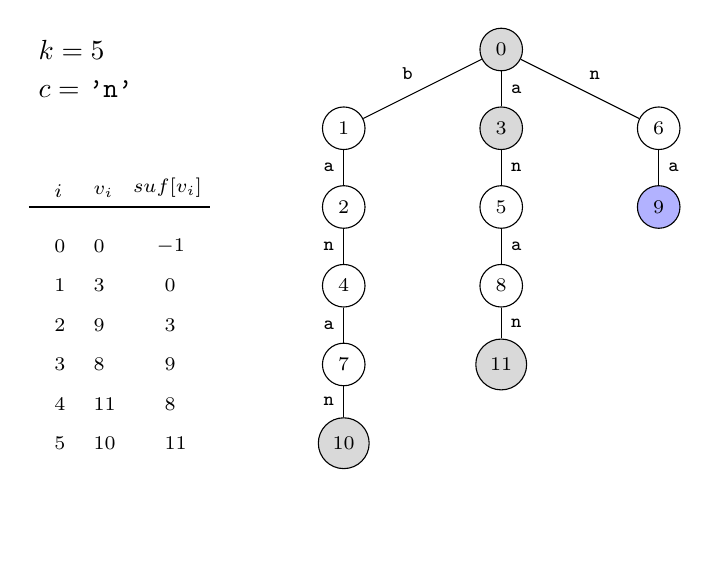
\begin{tikzpicture}
            \node[anchor=west] at (-2, 7) { $k = 5$ };
            \node[anchor=west,opacity=1] at (-2, 6.5) { $c = $ \texttt{'n'} };

            \node[anchor=south west] at (-1.8, 5) { \scriptsize $i$ };
            \node[anchor=south west] at (-1.3, 5) { \scriptsize $v_i$ };
            \node[anchor=south west] at (-0.8, 5) { \scriptsize $suf[v_i]$ };
            \draw[thick] (-2, 5) -- (0.3, 5);

            \node[anchor=west] at (-1.8, 4.5) { \scriptsize $0$ };
            \node[anchor=west] at (-1.3, 4.5) { \scriptsize $0$ };
            \node[anchor=west] at (-0.5, 4.5) { \scriptsize $-1$ };
            
            \node[anchor=west] at (-1.8, 4.0) { \scriptsize $1$ };
            \node[anchor=west] at (-1.3, 4.0) { \scriptsize \textcolor{black}{$3$} };
            \node[anchor=west] at (-0.4, 4.0) { \scriptsize $0$ };

            \node[anchor=west] at (-1.8, 3.5) { \scriptsize $2$ };
            \node[anchor=west] at (-1.3, 3.5) { \scriptsize \textcolor{black}{$9$} };
            \node[anchor=west] at (-0.4, 3.5) { \scriptsize \textcolor{black}{$3$} };

            \node[anchor=west] at (-1.8, 3.0) { \scriptsize $3$ };
            \node[anchor=west] at (-1.3, 3.0) { \scriptsize \textcolor{black}{$8$} };
            \node[anchor=west] at (-0.4, 3.0) { \scriptsize \textcolor{black}{$9$} };

            \node[anchor=west] at (-1.8, 2.5) { \scriptsize $4$ };
            \node[anchor=west] at (-1.3, 2.5) { \scriptsize \textcolor{black}{$11$} };
            \node[anchor=west] at (-0.4, 2.5) { \scriptsize \textcolor{black}{$8$} };

            \node[anchor=west] at (-1.8, 2.0) { \scriptsize $5$ };
            \node[anchor=west] at (-1.3, 2.0) { \scriptsize $10$ };
            \node[anchor=west] at (-0.4, 2.0) { \scriptsize \textcolor{black}{$11$} };

            \node[circle,draw,opacity=1,fill=gray!30] (A) at (4, 7) {\scriptsize 0};
            \node[circle,draw,opacity=1] (B1) at (2, 6) {\scriptsize 1};
            \node[circle,draw,opacity=1,fill=gray!30] (B2) at (4, 6) {\scriptsize 3};
            \node[circle,draw,opacity=1] (B3) at (6, 6) {\scriptsize 6};
            \node[circle,draw,opacity=1] (C1) at (2, 5) {\scriptsize 2};
            \node[circle,draw,opacity=1] (C2) at (4, 5) {\scriptsize 5};
            \node[circle,draw,opacity=1,fill=blue!30] (C3) at (6, 5) {\scriptsize 9};
            \node[circle,draw,opacity=1] (D1) at (2, 4) {\scriptsize 4};
            \node[circle,draw,opacity=1] (D2) at (4, 4) {\scriptsize 8};
            \node[circle,draw,opacity=0] (D3) at (6, 4) {\scriptsize 11};
            \node[circle,draw,opacity=1] (E1) at (2, 3) {\scriptsize 7};
            \node[circle,draw,opacity=1,fill=gray!30] (E2) at (4, 3) {\scriptsize 11};
            \node[circle,draw,opacity=0] (E3) at (6, 3) {\scriptsize 10};
            \node[circle,draw,opacity=1,fill=gray!30] (F1) at (2, 2) {\scriptsize 10};
            \node[circle,draw,opacity=0] (F2) at (4, 2) {\scriptsize 10};
            \node[circle,draw,opacity=0] (G1) at (2, 1) {\scriptsize 10};

            \draw (A) -- node[anchor=south east] { \tt \scriptsize b } (B1);
            \draw (A) -- node[anchor=west] { \tt \scriptsize a } (B2);
            \draw (A) -- node[anchor=south west] { \tt \scriptsize n } (B3);
            \draw (B1) -- node[anchor=east] { \tt \scriptsize a } (C1);
            \draw (B2) -- node[anchor=west] { \tt \scriptsize n } (C2);
            \draw (B3) -- node[anchor=west] { \tt \scriptsize a } (C3);
            \draw (C1) -- node[anchor=east] { \tt \scriptsize n } (D1);
            \draw (C2) -- node[anchor=west] { \tt \scriptsize a } (D2);
%            \draw (C3) -- node[anchor=west] { N } (D3);
            \draw (D1) -- node[anchor=east] { \tt \scriptsize a } (E1);
            \draw (D2) -- node[anchor=west] { \tt \scriptsize n } (E2);
%            \draw (D3) -- node[anchor=west] { A } (E3);
            \draw (E1) -- node[anchor=east] { \tt \scriptsize n } (F1);
%            \draw (E2) -- node[anchor=west] { A } (F2);
%            \draw (F1) -- node[anchor=east] { A } (G1);
%
%            \node[circle] (N1) at (G1) { };
%            \node[circle] (N2) at (F2) { };
%            \node[circle] (N3) at (E3) { };
%            \node[circle] (N4) at (D2) { };
%            \node[circle] (N5) at (C3) { };
%            \node[circle] (N6) at (B2) { };
%
%            \draw[dashed,->] (N1) -- (N2);
%            \draw[dashed,->] (N2) -- (N3);
%            \draw[dashed,->] (N3) -- (N4);
%            \draw[dashed,->] (N4) -- (N5);
%            \draw[dashed,->] (N5) -- (N6);
    \end{tikzpicture}
\end{frame}

\begin{frame}[fragile]{Visualização da construção {\it online} da {\it trie}}

    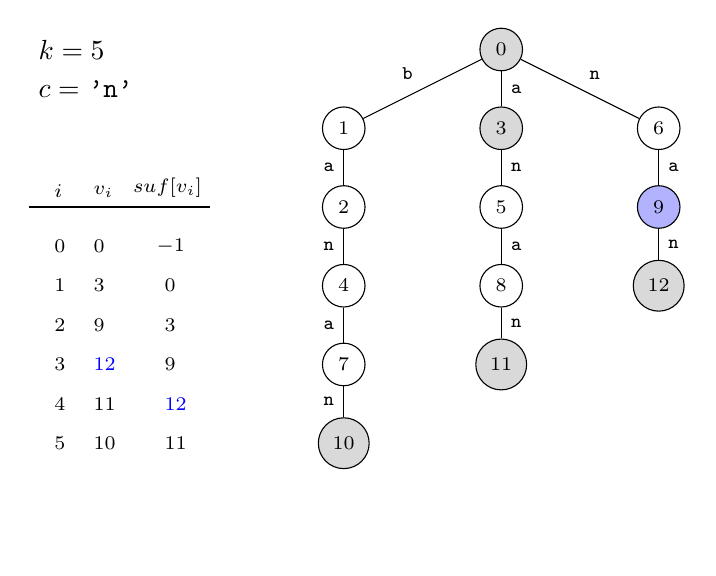
\begin{tikzpicture}
            \node[anchor=west] at (-2, 7) { $k = 5$ };
            \node[anchor=west,opacity=1] at (-2, 6.5) { $c = $ \texttt{'n'} };

            \node[anchor=south west] at (-1.8, 5) { \scriptsize $i$ };
            \node[anchor=south west] at (-1.3, 5) { \scriptsize $v_i$ };
            \node[anchor=south west] at (-0.8, 5) { \scriptsize $suf[v_i]$ };
            \draw[thick] (-2, 5) -- (0.3, 5);

            \node[anchor=west] at (-1.8, 4.5) { \scriptsize $0$ };
            \node[anchor=west] at (-1.3, 4.5) { \scriptsize $0$ };
            \node[anchor=west] at (-0.5, 4.5) { \scriptsize $-1$ };
            
            \node[anchor=west] at (-1.8, 4.0) { \scriptsize $1$ };
            \node[anchor=west] at (-1.3, 4.0) { \scriptsize \textcolor{black}{$3$} };
            \node[anchor=west] at (-0.4, 4.0) { \scriptsize $0$ };

            \node[anchor=west] at (-1.8, 3.5) { \scriptsize $2$ };
            \node[anchor=west] at (-1.3, 3.5) { \scriptsize \textcolor{black}{$9$} };
            \node[anchor=west] at (-0.4, 3.5) { \scriptsize \textcolor{black}{$3$} };

            \node[anchor=west] at (-1.8, 3.0) { \scriptsize $3$ };
            \node[anchor=west] at (-1.3, 3.0) { \scriptsize \textcolor{blue}{$12$} };
            \node[anchor=west] at (-0.4, 3.0) { \scriptsize \textcolor{black}{$9$} };

            \node[anchor=west] at (-1.8, 2.5) { \scriptsize $4$ };
            \node[anchor=west] at (-1.3, 2.5) { \scriptsize \textcolor{black}{$11$} };
            \node[anchor=west] at (-0.4, 2.5) { \scriptsize \textcolor{blue}{$12$} };

            \node[anchor=west] at (-1.8, 2.0) { \scriptsize $5$ };
            \node[anchor=west] at (-1.3, 2.0) { \scriptsize $10$ };
            \node[anchor=west] at (-0.4, 2.0) { \scriptsize \textcolor{black}{$11$} };

            \node[circle,draw,opacity=1,fill=gray!30] (A) at (4, 7) {\scriptsize 0};
            \node[circle,draw,opacity=1] (B1) at (2, 6) {\scriptsize 1};
            \node[circle,draw,opacity=1,fill=gray!30] (B2) at (4, 6) {\scriptsize 3};
            \node[circle,draw,opacity=1] (B3) at (6, 6) {\scriptsize 6};
            \node[circle,draw,opacity=1] (C1) at (2, 5) {\scriptsize 2};
            \node[circle,draw,opacity=1] (C2) at (4, 5) {\scriptsize 5};
            \node[circle,draw,opacity=1,fill=blue!30] (C3) at (6, 5) {\scriptsize 9};
            \node[circle,draw,opacity=1] (D1) at (2, 4) {\scriptsize 4};
            \node[circle,draw,opacity=1] (D2) at (4, 4) {\scriptsize 8};
            \node[circle,draw,opacity=1,fill=gray!30] (D3) at (6, 4) {\scriptsize 12};
            \node[circle,draw,opacity=1] (E1) at (2, 3) {\scriptsize 7};
            \node[circle,draw,opacity=1,fill=gray!30] (E2) at (4, 3) {\scriptsize 11};
            \node[circle,draw,opacity=0] (E3) at (6, 3) {\scriptsize 10};
            \node[circle,draw,opacity=1,fill=gray!30] (F1) at (2, 2) {\scriptsize 10};
            \node[circle,draw,opacity=0] (F2) at (4, 2) {\scriptsize 10};
            \node[circle,draw,opacity=0] (G1) at (2, 1) {\scriptsize 10};

            \draw (A) -- node[anchor=south east] { \tt \scriptsize b } (B1);
            \draw (A) -- node[anchor=west] { \tt \scriptsize a } (B2);
            \draw (A) -- node[anchor=south west] { \tt \scriptsize n } (B3);
            \draw (B1) -- node[anchor=east] { \tt \scriptsize a } (C1);
            \draw (B2) -- node[anchor=west] { \tt \scriptsize n } (C2);
            \draw (B3) -- node[anchor=west] { \tt \scriptsize a } (C3);
            \draw (C1) -- node[anchor=east] { \tt \scriptsize n } (D1);
            \draw (C2) -- node[anchor=west] { \tt \scriptsize a } (D2);
            \draw (C3) -- node[anchor=west] { \tt \scriptsize n } (D3);
            \draw (D1) -- node[anchor=east] { \tt \scriptsize a } (E1);
            \draw (D2) -- node[anchor=west] { \tt \scriptsize n } (E2);
%            \draw (D3) -- node[anchor=west] { A } (E3);
            \draw (E1) -- node[anchor=east] { \tt \scriptsize n } (F1);
%            \draw (E2) -- node[anchor=west] { A } (F2);
%            \draw (F1) -- node[anchor=east] { A } (G1);
%
%            \node[circle] (N1) at (G1) { };
%            \node[circle] (N2) at (F2) { };
%            \node[circle] (N3) at (E3) { };
%            \node[circle] (N4) at (D2) { };
%            \node[circle] (N5) at (C3) { };
%            \node[circle] (N6) at (B2) { };
%
%            \draw[dashed,->] (N1) -- (N2);
%            \draw[dashed,->] (N2) -- (N3);
%            \draw[dashed,->] (N3) -- (N4);
%            \draw[dashed,->] (N4) -- (N5);
%            \draw[dashed,->] (N5) -- (N6);
    \end{tikzpicture}
\end{frame}

\begin{frame}[fragile]{Visualização da construção {\it online} da {\it trie}}

    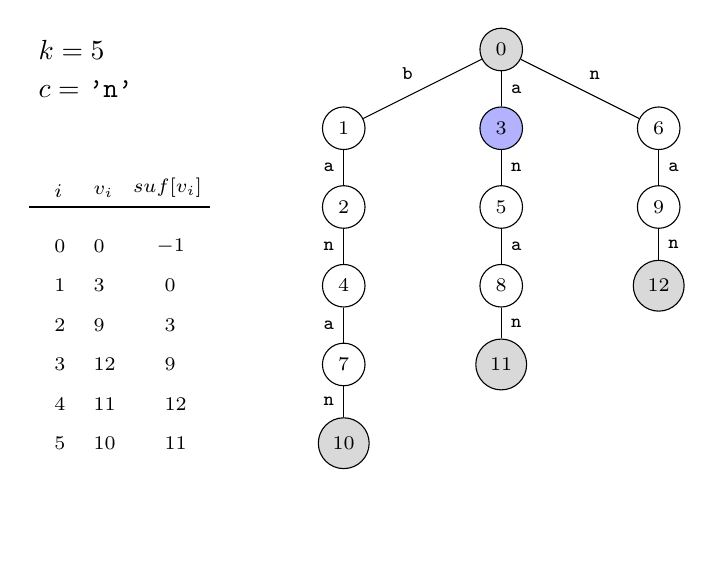
\begin{tikzpicture}
            \node[anchor=west] at (-2, 7) { $k = 5$ };
            \node[anchor=west,opacity=1] at (-2, 6.5) { $c = $ \texttt{'n'} };

            \node[anchor=south west] at (-1.8, 5) { \scriptsize $i$ };
            \node[anchor=south west] at (-1.3, 5) { \scriptsize $v_i$ };
            \node[anchor=south west] at (-0.8, 5) { \scriptsize $suf[v_i]$ };
            \draw[thick] (-2, 5) -- (0.3, 5);

            \node[anchor=west] at (-1.8, 4.5) { \scriptsize $0$ };
            \node[anchor=west] at (-1.3, 4.5) { \scriptsize $0$ };
            \node[anchor=west] at (-0.5, 4.5) { \scriptsize $-1$ };
            
            \node[anchor=west] at (-1.8, 4.0) { \scriptsize $1$ };
            \node[anchor=west] at (-1.3, 4.0) { \scriptsize \textcolor{black}{$3$} };
            \node[anchor=west] at (-0.4, 4.0) { \scriptsize $0$ };

            \node[anchor=west] at (-1.8, 3.5) { \scriptsize $2$ };
            \node[anchor=west] at (-1.3, 3.5) { \scriptsize \textcolor{black}{$9$} };
            \node[anchor=west] at (-0.4, 3.5) { \scriptsize \textcolor{black}{$3$} };

            \node[anchor=west] at (-1.8, 3.0) { \scriptsize $3$ };
            \node[anchor=west] at (-1.3, 3.0) { \scriptsize \textcolor{black}{$12$} };
            \node[anchor=west] at (-0.4, 3.0) { \scriptsize \textcolor{black}{$9$} };

            \node[anchor=west] at (-1.8, 2.5) { \scriptsize $4$ };
            \node[anchor=west] at (-1.3, 2.5) { \scriptsize \textcolor{black}{$11$} };
            \node[anchor=west] at (-0.4, 2.5) { \scriptsize \textcolor{black}{$12$} };

            \node[anchor=west] at (-1.8, 2.0) { \scriptsize $5$ };
            \node[anchor=west] at (-1.3, 2.0) { \scriptsize $10$ };
            \node[anchor=west] at (-0.4, 2.0) { \scriptsize \textcolor{black}{$11$} };

            \node[circle,draw,opacity=1,fill=gray!30] (A) at (4, 7) {\scriptsize 0};
            \node[circle,draw,opacity=1] (B1) at (2, 6) {\scriptsize 1};
            \node[circle,draw,opacity=1,fill=blue!30] (B2) at (4, 6) {\scriptsize 3};
            \node[circle,draw,opacity=1] (B3) at (6, 6) {\scriptsize 6};
            \node[circle,draw,opacity=1] (C1) at (2, 5) {\scriptsize 2};
            \node[circle,draw,opacity=1] (C2) at (4, 5) {\scriptsize 5};
            \node[circle,draw,opacity=1] (C3) at (6, 5) {\scriptsize 9};
            \node[circle,draw,opacity=1] (D1) at (2, 4) {\scriptsize 4};
            \node[circle,draw,opacity=1] (D2) at (4, 4) {\scriptsize 8};
            \node[circle,draw,opacity=1,fill=gray!30] (D3) at (6, 4) {\scriptsize 12};
            \node[circle,draw,opacity=1] (E1) at (2, 3) {\scriptsize 7};
            \node[circle,draw,opacity=1,fill=gray!30] (E2) at (4, 3) {\scriptsize 11};
            \node[circle,draw,opacity=0] (E3) at (6, 3) {\scriptsize 10};
            \node[circle,draw,opacity=1,fill=gray!30] (F1) at (2, 2) {\scriptsize 10};
            \node[circle,draw,opacity=0] (F2) at (4, 2) {\scriptsize 10};
            \node[circle,draw,opacity=0] (G1) at (2, 1) {\scriptsize 10};

            \draw (A) -- node[anchor=south east] { \tt \scriptsize b } (B1);
            \draw (A) -- node[anchor=west] { \tt \scriptsize a } (B2);
            \draw (A) -- node[anchor=south west] { \tt \scriptsize n } (B3);
            \draw (B1) -- node[anchor=east] { \tt \scriptsize a } (C1);
            \draw (B2) -- node[anchor=west] { \tt \scriptsize n } (C2);
            \draw (B3) -- node[anchor=west] { \tt \scriptsize a } (C3);
            \draw (C1) -- node[anchor=east] { \tt \scriptsize n } (D1);
            \draw (C2) -- node[anchor=west] { \tt \scriptsize a } (D2);
            \draw (C3) -- node[anchor=west] { \tt \scriptsize n } (D3);
            \draw (D1) -- node[anchor=east] { \tt \scriptsize a } (E1);
            \draw (D2) -- node[anchor=west] { \tt \scriptsize n } (E2);
%            \draw (D3) -- node[anchor=west] { A } (E3);
            \draw (E1) -- node[anchor=east] { \tt \scriptsize n } (F1);
%            \draw (E2) -- node[anchor=west] { A } (F2);
%            \draw (F1) -- node[anchor=east] { A } (G1);
%
%            \node[circle] (N1) at (G1) { };
%            \node[circle] (N2) at (F2) { };
%            \node[circle] (N3) at (E3) { };
%            \node[circle] (N4) at (D2) { };
%            \node[circle] (N5) at (C3) { };
%            \node[circle] (N6) at (B2) { };
%
%            \draw[dashed,->] (N1) -- (N2);
%            \draw[dashed,->] (N2) -- (N3);
%            \draw[dashed,->] (N3) -- (N4);
%            \draw[dashed,->] (N4) -- (N5);
%            \draw[dashed,->] (N5) -- (N6);
    \end{tikzpicture}
\end{frame}

\begin{frame}[fragile]{Visualização da construção {\it online} da {\it trie}}

    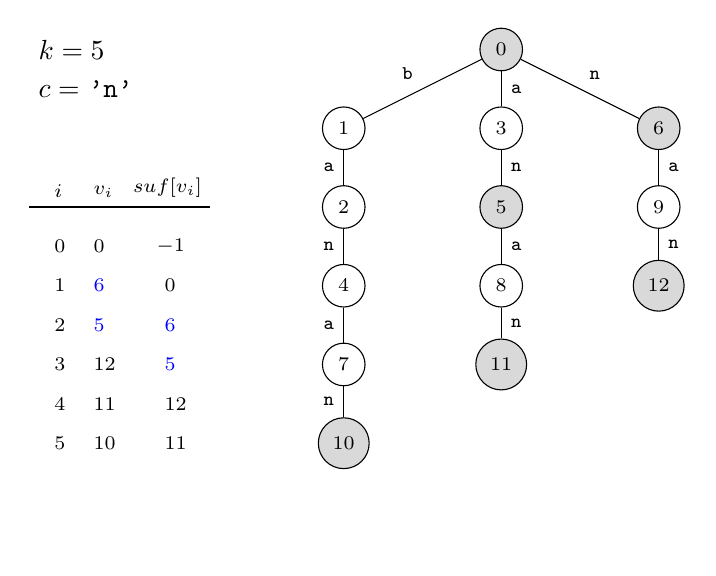
\begin{tikzpicture}
            \node[anchor=west] at (-2, 7) { $k = 5$ };
            \node[anchor=west,opacity=1] at (-2, 6.5) { $c = $ \texttt{'n'} };

            \node[anchor=south west] at (-1.8, 5) { \scriptsize $i$ };
            \node[anchor=south west] at (-1.3, 5) { \scriptsize $v_i$ };
            \node[anchor=south west] at (-0.8, 5) { \scriptsize $suf[v_i]$ };
            \draw[thick] (-2, 5) -- (0.3, 5);

            \node[anchor=west] at (-1.8, 4.5) { \scriptsize $0$ };
            \node[anchor=west] at (-1.3, 4.5) { \scriptsize $0$ };
            \node[anchor=west] at (-0.5, 4.5) { \scriptsize $-1$ };
            
            \node[anchor=west] at (-1.8, 4.0) { \scriptsize $1$ };
            \node[anchor=west] at (-1.3, 4.0) { \scriptsize \textcolor{blue}{$6$} };
            \node[anchor=west] at (-0.4, 4.0) { \scriptsize $0$ };

            \node[anchor=west] at (-1.8, 3.5) { \scriptsize $2$ };
            \node[anchor=west] at (-1.3, 3.5) { \scriptsize \textcolor{blue}{$5$} };
            \node[anchor=west] at (-0.4, 3.5) { \scriptsize \textcolor{blue}{$6$} };

            \node[anchor=west] at (-1.8, 3.0) { \scriptsize $3$ };
            \node[anchor=west] at (-1.3, 3.0) { \scriptsize \textcolor{black}{$12$} };
            \node[anchor=west] at (-0.4, 3.0) { \scriptsize \textcolor{blue}{$5$} };

            \node[anchor=west] at (-1.8, 2.5) { \scriptsize $4$ };
            \node[anchor=west] at (-1.3, 2.5) { \scriptsize \textcolor{black}{$11$} };
            \node[anchor=west] at (-0.4, 2.5) { \scriptsize \textcolor{black}{$12$} };

            \node[anchor=west] at (-1.8, 2.0) { \scriptsize $5$ };
            \node[anchor=west] at (-1.3, 2.0) { \scriptsize $10$ };
            \node[anchor=west] at (-0.4, 2.0) { \scriptsize \textcolor{black}{$11$} };

            \node[circle,draw,opacity=1,fill=gray!30] (A) at (4, 7) {\scriptsize 0};
            \node[circle,draw,opacity=1] (B1) at (2, 6) {\scriptsize 1};
            \node[circle,draw,opacity=1] (B2) at (4, 6) {\scriptsize 3};
            \node[circle,draw,opacity=1,fill=gray!30] (B3) at (6, 6) {\scriptsize 6};
            \node[circle,draw,opacity=1] (C1) at (2, 5) {\scriptsize 2};
            \node[circle,draw,opacity=1,fill=gray!30] (C2) at (4, 5) {\scriptsize 5};
            \node[circle,draw,opacity=1] (C3) at (6, 5) {\scriptsize 9};
            \node[circle,draw,opacity=1] (D1) at (2, 4) {\scriptsize 4};
            \node[circle,draw,opacity=1] (D2) at (4, 4) {\scriptsize 8};
            \node[circle,draw,opacity=1,fill=gray!30] (D3) at (6, 4) {\scriptsize 12};
            \node[circle,draw,opacity=1] (E1) at (2, 3) {\scriptsize 7};
            \node[circle,draw,opacity=1,fill=gray!30] (E2) at (4, 3) {\scriptsize 11};
            \node[circle,draw,opacity=0] (E3) at (6, 3) {\scriptsize 10};
            \node[circle,draw,opacity=1,fill=gray!30] (F1) at (2, 2) {\scriptsize 10};
            \node[circle,draw,opacity=0] (F2) at (4, 2) {\scriptsize 10};
            \node[circle,draw,opacity=0] (G1) at (2, 1) {\scriptsize 10};

            \draw (A) -- node[anchor=south east] { \tt \scriptsize b } (B1);
            \draw (A) -- node[anchor=west] { \tt \scriptsize a } (B2);
            \draw (A) -- node[anchor=south west] { \tt \scriptsize n } (B3);
            \draw (B1) -- node[anchor=east] { \tt \scriptsize a } (C1);
            \draw (B2) -- node[anchor=west] { \tt \scriptsize n } (C2);
            \draw (B3) -- node[anchor=west] { \tt \scriptsize a } (C3);
            \draw (C1) -- node[anchor=east] { \tt \scriptsize n } (D1);
            \draw (C2) -- node[anchor=west] { \tt \scriptsize a } (D2);
            \draw (C3) -- node[anchor=west] { \tt \scriptsize n } (D3);
            \draw (D1) -- node[anchor=east] { \tt \scriptsize a } (E1);
            \draw (D2) -- node[anchor=west] { \tt \scriptsize n } (E2);
%            \draw (D3) -- node[anchor=west] { A } (E3);
            \draw (E1) -- node[anchor=east] { \tt \scriptsize n } (F1);
%            \draw (E2) -- node[anchor=west] { A } (F2);
%            \draw (F1) -- node[anchor=east] { A } (G1);
%
%            \node[circle] (N1) at (G1) { };
%            \node[circle] (N2) at (F2) { };
%            \node[circle] (N3) at (E3) { };
%            \node[circle] (N4) at (D2) { };
%            \node[circle] (N5) at (C3) { };
%            \node[circle] (N6) at (B2) { };
%
%            \draw[dashed,->] (N1) -- (N2);
%            \draw[dashed,->] (N2) -- (N3);
%            \draw[dashed,->] (N3) -- (N4);
%            \draw[dashed,->] (N4) -- (N5);
%            \draw[dashed,->] (N5) -- (N6);
    \end{tikzpicture}
\end{frame}

\begin{frame}[fragile]{Visualização da construção {\it online} da {\it trie}}

    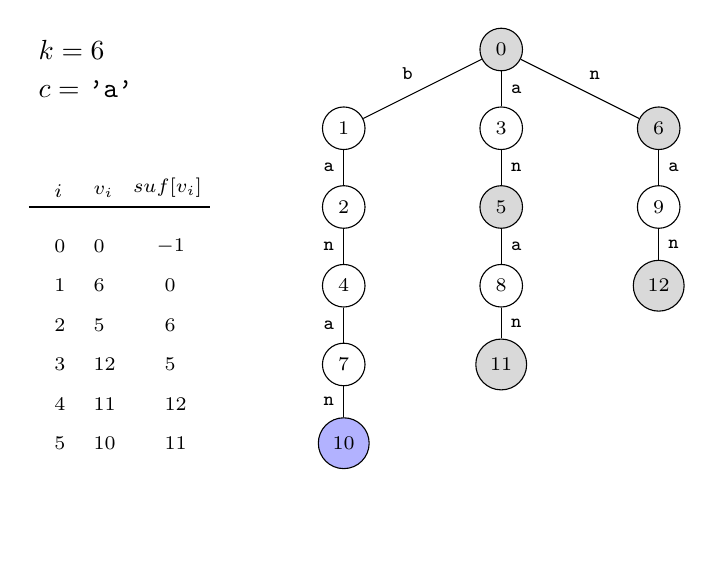
\begin{tikzpicture}
            \node[anchor=west] at (-2, 7) { $k = 6$ };
            \node[anchor=west,opacity=1] at (-2, 6.5) { $c = $ \texttt{'a'} };

            \node[anchor=south west] at (-1.8, 5) { \scriptsize $i$ };
            \node[anchor=south west] at (-1.3, 5) { \scriptsize $v_i$ };
            \node[anchor=south west] at (-0.8, 5) { \scriptsize $suf[v_i]$ };
            \draw[thick] (-2, 5) -- (0.3, 5);

            \node[anchor=west] at (-1.8, 4.5) { \scriptsize $0$ };
            \node[anchor=west] at (-1.3, 4.5) { \scriptsize $0$ };
            \node[anchor=west] at (-0.5, 4.5) { \scriptsize $-1$ };
            
            \node[anchor=west] at (-1.8, 4.0) { \scriptsize $1$ };
            \node[anchor=west] at (-1.3, 4.0) { \scriptsize \textcolor{black}{$6$} };
            \node[anchor=west] at (-0.4, 4.0) { \scriptsize $0$ };

            \node[anchor=west] at (-1.8, 3.5) { \scriptsize $2$ };
            \node[anchor=west] at (-1.3, 3.5) { \scriptsize \textcolor{black}{$5$} };
            \node[anchor=west] at (-0.4, 3.5) { \scriptsize \textcolor{black}{$6$} };

            \node[anchor=west] at (-1.8, 3.0) { \scriptsize $3$ };
            \node[anchor=west] at (-1.3, 3.0) { \scriptsize \textcolor{black}{$12$} };
            \node[anchor=west] at (-0.4, 3.0) { \scriptsize \textcolor{black}{$5$} };

            \node[anchor=west] at (-1.8, 2.5) { \scriptsize $4$ };
            \node[anchor=west] at (-1.3, 2.5) { \scriptsize \textcolor{black}{$11$} };
            \node[anchor=west] at (-0.4, 2.5) { \scriptsize \textcolor{black}{$12$} };

            \node[anchor=west] at (-1.8, 2.0) { \scriptsize $5$ };
            \node[anchor=west] at (-1.3, 2.0) { \scriptsize $10$ };
            \node[anchor=west] at (-0.4, 2.0) { \scriptsize \textcolor{black}{$11$} };

            \node[circle,draw,opacity=1,fill=gray!30] (A) at (4, 7) {\scriptsize 0};
            \node[circle,draw,opacity=1] (B1) at (2, 6) {\scriptsize 1};
            \node[circle,draw,opacity=1] (B2) at (4, 6) {\scriptsize 3};
            \node[circle,draw,opacity=1,fill=gray!30] (B3) at (6, 6) {\scriptsize 6};
            \node[circle,draw,opacity=1] (C1) at (2, 5) {\scriptsize 2};
            \node[circle,draw,opacity=1,fill=gray!30] (C2) at (4, 5) {\scriptsize 5};
            \node[circle,draw,opacity=1] (C3) at (6, 5) {\scriptsize 9};
            \node[circle,draw,opacity=1] (D1) at (2, 4) {\scriptsize 4};
            \node[circle,draw,opacity=1] (D2) at (4, 4) {\scriptsize 8};
            \node[circle,draw,opacity=1,fill=gray!30] (D3) at (6, 4) {\scriptsize 12};
            \node[circle,draw,opacity=1] (E1) at (2, 3) {\scriptsize 7};
            \node[circle,draw,opacity=1,fill=gray!30] (E2) at (4, 3) {\scriptsize 11};
            \node[circle,draw,opacity=0] (E3) at (6, 3) {\scriptsize 10};
            \node[circle,draw,opacity=1,fill=blue!30] (F1) at (2, 2) {\scriptsize 10};
            \node[circle,draw,opacity=0] (F2) at (4, 2) {\scriptsize 10};
            \node[circle,draw,opacity=0] (G1) at (2, 1) {\scriptsize 10};

            \draw (A) -- node[anchor=south east] { \tt \scriptsize b } (B1);
            \draw (A) -- node[anchor=west] { \tt \scriptsize a } (B2);
            \draw (A) -- node[anchor=south west] { \tt \scriptsize n } (B3);
            \draw (B1) -- node[anchor=east] { \tt \scriptsize a } (C1);
            \draw (B2) -- node[anchor=west] { \tt \scriptsize n } (C2);
            \draw (B3) -- node[anchor=west] { \tt \scriptsize a } (C3);
            \draw (C1) -- node[anchor=east] { \tt \scriptsize n } (D1);
            \draw (C2) -- node[anchor=west] { \tt \scriptsize a } (D2);
            \draw (C3) -- node[anchor=west] { \tt \scriptsize n } (D3);
            \draw (D1) -- node[anchor=east] { \tt \scriptsize a } (E1);
            \draw (D2) -- node[anchor=west] { \tt \scriptsize n } (E2);
%            \draw (D3) -- node[anchor=west] { A } (E3);
            \draw (E1) -- node[anchor=east] { \tt \scriptsize n } (F1);
%            \draw (E2) -- node[anchor=west] { A } (F2);
%            \draw (F1) -- node[anchor=east] { A } (G1);
%
%            \node[circle] (N1) at (G1) { };
%            \node[circle] (N2) at (F2) { };
%            \node[circle] (N3) at (E3) { };
%            \node[circle] (N4) at (D2) { };
%            \node[circle] (N5) at (C3) { };
%            \node[circle] (N6) at (B2) { };
%
%            \draw[dashed,->] (N1) -- (N2);
%            \draw[dashed,->] (N2) -- (N3);
%            \draw[dashed,->] (N3) -- (N4);
%            \draw[dashed,->] (N4) -- (N5);
%            \draw[dashed,->] (N5) -- (N6);
    \end{tikzpicture}
\end{frame}

\begin{frame}[fragile]{Visualização da construção {\it online} da {\it trie}}

    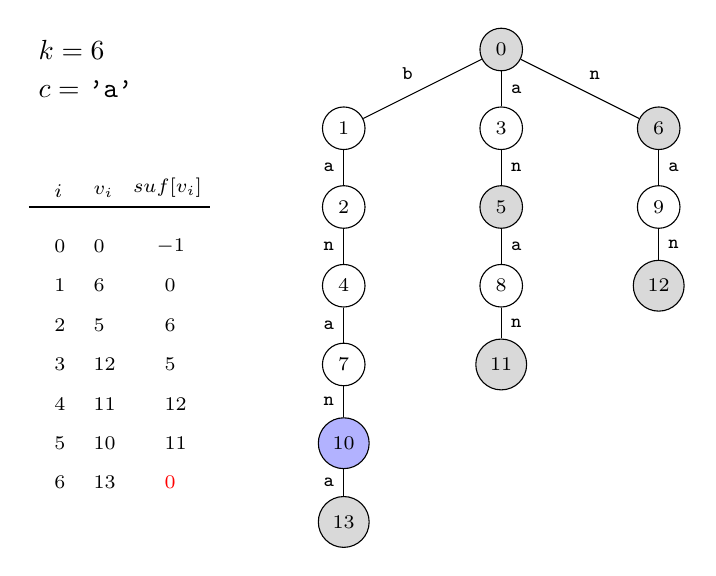
\begin{tikzpicture}
            \node[anchor=west] at (-2, 7) { $k = 6$ };
            \node[anchor=west,opacity=1] at (-2, 6.5) { $c = $ \texttt{'a'} };

            \node[anchor=south west] at (-1.8, 5) { \scriptsize $i$ };
            \node[anchor=south west] at (-1.3, 5) { \scriptsize $v_i$ };
            \node[anchor=south west] at (-0.8, 5) { \scriptsize $suf[v_i]$ };
            \draw[thick] (-2, 5) -- (0.3, 5);

            \node[anchor=west] at (-1.8, 4.5) { \scriptsize $0$ };
            \node[anchor=west] at (-1.3, 4.5) { \scriptsize $0$ };
            \node[anchor=west] at (-0.5, 4.5) { \scriptsize $-1$ };
            
            \node[anchor=west] at (-1.8, 4.0) { \scriptsize $1$ };
            \node[anchor=west] at (-1.3, 4.0) { \scriptsize \textcolor{black}{$6$} };
            \node[anchor=west] at (-0.4, 4.0) { \scriptsize $0$ };

            \node[anchor=west] at (-1.8, 3.5) { \scriptsize $2$ };
            \node[anchor=west] at (-1.3, 3.5) { \scriptsize \textcolor{black}{$5$} };
            \node[anchor=west] at (-0.4, 3.5) { \scriptsize \textcolor{black}{$6$} };

            \node[anchor=west] at (-1.8, 3.0) { \scriptsize $3$ };
            \node[anchor=west] at (-1.3, 3.0) { \scriptsize \textcolor{black}{$12$} };
            \node[anchor=west] at (-0.4, 3.0) { \scriptsize \textcolor{black}{$5$} };

            \node[anchor=west] at (-1.8, 2.5) { \scriptsize $4$ };
            \node[anchor=west] at (-1.3, 2.5) { \scriptsize \textcolor{black}{$11$} };
            \node[anchor=west] at (-0.4, 2.5) { \scriptsize \textcolor{black}{$12$} };

            \node[anchor=west] at (-1.8, 2.0) { \scriptsize $5$ };
            \node[anchor=west] at (-1.3, 2.0) { \scriptsize $10$ };
            \node[anchor=west] at (-0.4, 2.0) { \scriptsize \textcolor{black}{$11$} };

            \node[anchor=west] at (-1.8, 1.5) { \scriptsize $6$ };
            \node[anchor=west] at (-1.3, 1.5) { \scriptsize $13$ };
            \node[anchor=west] at (-0.4, 1.5) { \scriptsize \textcolor{red}{$0$} };

            \node[circle,draw,opacity=1,fill=gray!30] (A) at (4, 7) {\scriptsize 0};
            \node[circle,draw,opacity=1] (B1) at (2, 6) {\scriptsize 1};
            \node[circle,draw,opacity=1] (B2) at (4, 6) {\scriptsize 3};
            \node[circle,draw,opacity=1,fill=gray!30] (B3) at (6, 6) {\scriptsize 6};
            \node[circle,draw,opacity=1] (C1) at (2, 5) {\scriptsize 2};
            \node[circle,draw,opacity=1,fill=gray!30] (C2) at (4, 5) {\scriptsize 5};
            \node[circle,draw,opacity=1] (C3) at (6, 5) {\scriptsize 9};
            \node[circle,draw,opacity=1] (D1) at (2, 4) {\scriptsize 4};
            \node[circle,draw,opacity=1] (D2) at (4, 4) {\scriptsize 8};
            \node[circle,draw,opacity=1,fill=gray!30] (D3) at (6, 4) {\scriptsize 12};
            \node[circle,draw,opacity=1] (E1) at (2, 3) {\scriptsize 7};
            \node[circle,draw,opacity=1,fill=gray!30] (E2) at (4, 3) {\scriptsize 11};
            \node[circle,draw,opacity=0] (E3) at (6, 3) {\scriptsize 10};
            \node[circle,draw,opacity=1,fill=blue!30] (F1) at (2, 2) {\scriptsize 10};
            \node[circle,draw,opacity=0] (F2) at (4, 2) {\scriptsize 10};
            \node[circle,draw,opacity=1,fill=gray!30] (G1) at (2, 1) {\scriptsize 13};

            \draw (A) -- node[anchor=south east] { \tt \scriptsize b } (B1);
            \draw (A) -- node[anchor=west] { \tt \scriptsize a } (B2);
            \draw (A) -- node[anchor=south west] { \tt \scriptsize n } (B3);
            \draw (B1) -- node[anchor=east] { \tt \scriptsize a } (C1);
            \draw (B2) -- node[anchor=west] { \tt \scriptsize n } (C2);
            \draw (B3) -- node[anchor=west] { \tt \scriptsize a } (C3);
            \draw (C1) -- node[anchor=east] { \tt \scriptsize n } (D1);
            \draw (C2) -- node[anchor=west] { \tt \scriptsize a } (D2);
            \draw (C3) -- node[anchor=west] { \tt \scriptsize n } (D3);
            \draw (D1) -- node[anchor=east] { \tt \scriptsize a } (E1);
            \draw (D2) -- node[anchor=west] { \tt \scriptsize n } (E2);
%            \draw (D3) -- node[anchor=west] { A } (E3);
            \draw (E1) -- node[anchor=east] { \tt \scriptsize n } (F1);
%            \draw (E2) -- node[anchor=west] { A } (F2);
            \draw (F1) -- node[anchor=east] { \tt \scriptsize a } (G1);
%
%            \node[circle] (N1) at (G1) { };
%            \node[circle] (N2) at (F2) { };
%            \node[circle] (N3) at (E3) { };
%            \node[circle] (N4) at (D2) { };
%            \node[circle] (N5) at (C3) { };
%            \node[circle] (N6) at (B2) { };
%
%            \draw[dashed,->] (N1) -- (N2);
%            \draw[dashed,->] (N2) -- (N3);
%            \draw[dashed,->] (N3) -- (N4);
%            \draw[dashed,->] (N4) -- (N5);
%            \draw[dashed,->] (N5) -- (N6);
    \end{tikzpicture}
\end{frame}

\begin{frame}[fragile]{Visualização da construção {\it online} da {\it trie}}

    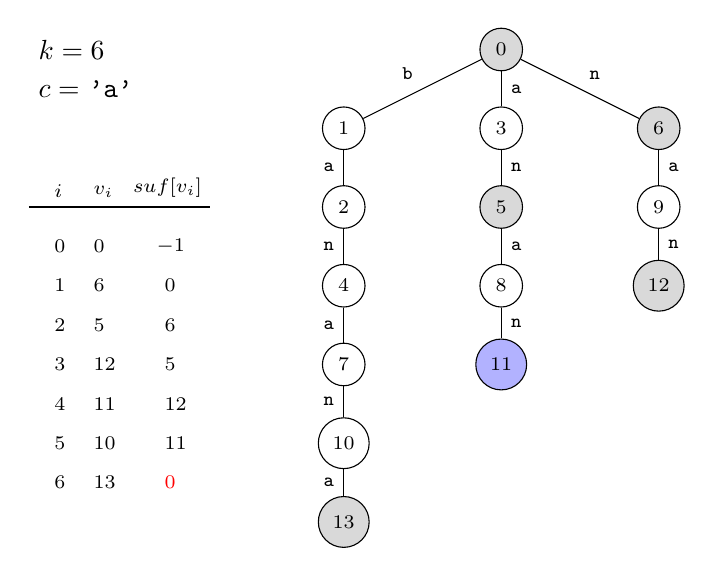
\begin{tikzpicture}
            \node[anchor=west] at (-2, 7) { $k = 6$ };
            \node[anchor=west,opacity=1] at (-2, 6.5) { $c = $ \texttt{'a'} };

            \node[anchor=south west] at (-1.8, 5) { \scriptsize $i$ };
            \node[anchor=south west] at (-1.3, 5) { \scriptsize $v_i$ };
            \node[anchor=south west] at (-0.8, 5) { \scriptsize $suf[v_i]$ };
            \draw[thick] (-2, 5) -- (0.3, 5);

            \node[anchor=west] at (-1.8, 4.5) { \scriptsize $0$ };
            \node[anchor=west] at (-1.3, 4.5) { \scriptsize $0$ };
            \node[anchor=west] at (-0.5, 4.5) { \scriptsize $-1$ };
            
            \node[anchor=west] at (-1.8, 4.0) { \scriptsize $1$ };
            \node[anchor=west] at (-1.3, 4.0) { \scriptsize \textcolor{black}{$6$} };
            \node[anchor=west] at (-0.4, 4.0) { \scriptsize $0$ };

            \node[anchor=west] at (-1.8, 3.5) { \scriptsize $2$ };
            \node[anchor=west] at (-1.3, 3.5) { \scriptsize \textcolor{black}{$5$} };
            \node[anchor=west] at (-0.4, 3.5) { \scriptsize \textcolor{black}{$6$} };

            \node[anchor=west] at (-1.8, 3.0) { \scriptsize $3$ };
            \node[anchor=west] at (-1.3, 3.0) { \scriptsize \textcolor{black}{$12$} };
            \node[anchor=west] at (-0.4, 3.0) { \scriptsize \textcolor{black}{$5$} };

            \node[anchor=west] at (-1.8, 2.5) { \scriptsize $4$ };
            \node[anchor=west] at (-1.3, 2.5) { \scriptsize \textcolor{black}{$11$} };
            \node[anchor=west] at (-0.4, 2.5) { \scriptsize \textcolor{black}{$12$} };

            \node[anchor=west] at (-1.8, 2.0) { \scriptsize $5$ };
            \node[anchor=west] at (-1.3, 2.0) { \scriptsize $10$ };
            \node[anchor=west] at (-0.4, 2.0) { \scriptsize \textcolor{black}{$11$} };

            \node[anchor=west] at (-1.8, 1.5) { \scriptsize $6$ };
            \node[anchor=west] at (-1.3, 1.5) { \scriptsize $13$ };
            \node[anchor=west] at (-0.4, 1.5) { \scriptsize \textcolor{red}{$0$} };

            \node[circle,draw,opacity=1,fill=gray!30] (A) at (4, 7) {\scriptsize 0};
            \node[circle,draw,opacity=1] (B1) at (2, 6) {\scriptsize 1};
            \node[circle,draw,opacity=1] (B2) at (4, 6) {\scriptsize 3};
            \node[circle,draw,opacity=1,fill=gray!30] (B3) at (6, 6) {\scriptsize 6};
            \node[circle,draw,opacity=1] (C1) at (2, 5) {\scriptsize 2};
            \node[circle,draw,opacity=1,fill=gray!30] (C2) at (4, 5) {\scriptsize 5};
            \node[circle,draw,opacity=1] (C3) at (6, 5) {\scriptsize 9};
            \node[circle,draw,opacity=1] (D1) at (2, 4) {\scriptsize 4};
            \node[circle,draw,opacity=1] (D2) at (4, 4) {\scriptsize 8};
            \node[circle,draw,opacity=1,fill=gray!30] (D3) at (6, 4) {\scriptsize 12};
            \node[circle,draw,opacity=1] (E1) at (2, 3) {\scriptsize 7};
            \node[circle,draw,opacity=1,fill=blue!30] (E2) at (4, 3) {\scriptsize 11};
            \node[circle,draw,opacity=0] (E3) at (6, 3) {\scriptsize 10};
            \node[circle,draw,opacity=1] (F1) at (2, 2) {\scriptsize 10};
            \node[circle,draw,opacity=0] (F2) at (4, 2) {\scriptsize 10};
            \node[circle,draw,opacity=1,fill=gray!30] (G1) at (2, 1) {\scriptsize 13};

            \draw (A) -- node[anchor=south east] { \tt \scriptsize b } (B1);
            \draw (A) -- node[anchor=west] { \tt \scriptsize a } (B2);
            \draw (A) -- node[anchor=south west] { \tt \scriptsize n } (B3);
            \draw (B1) -- node[anchor=east] { \tt \scriptsize a } (C1);
            \draw (B2) -- node[anchor=west] { \tt \scriptsize n } (C2);
            \draw (B3) -- node[anchor=west] { \tt \scriptsize a } (C3);
            \draw (C1) -- node[anchor=east] { \tt \scriptsize n } (D1);
            \draw (C2) -- node[anchor=west] { \tt \scriptsize a } (D2);
            \draw (C3) -- node[anchor=west] { \tt \scriptsize n } (D3);
            \draw (D1) -- node[anchor=east] { \tt \scriptsize a } (E1);
            \draw (D2) -- node[anchor=west] { \tt \scriptsize n } (E2);
%            \draw (D3) -- node[anchor=west] { A } (E3);
            \draw (E1) -- node[anchor=east] { \tt \scriptsize n } (F1);
%            \draw (E2) -- node[anchor=west] { A } (F2);
            \draw (F1) -- node[anchor=east] { \tt \scriptsize a } (G1);
%
%            \node[circle] (N1) at (G1) { };
%            \node[circle] (N2) at (F2) { };
%            \node[circle] (N3) at (E3) { };
%            \node[circle] (N4) at (D2) { };
%            \node[circle] (N5) at (C3) { };
%            \node[circle] (N6) at (B2) { };
%
%            \draw[dashed,->] (N1) -- (N2);
%            \draw[dashed,->] (N2) -- (N3);
%            \draw[dashed,->] (N3) -- (N4);
%            \draw[dashed,->] (N4) -- (N5);
%            \draw[dashed,->] (N5) -- (N6);
    \end{tikzpicture}
\end{frame}

\begin{frame}[fragile]{Visualização da construção {\it online} da {\it trie}}

    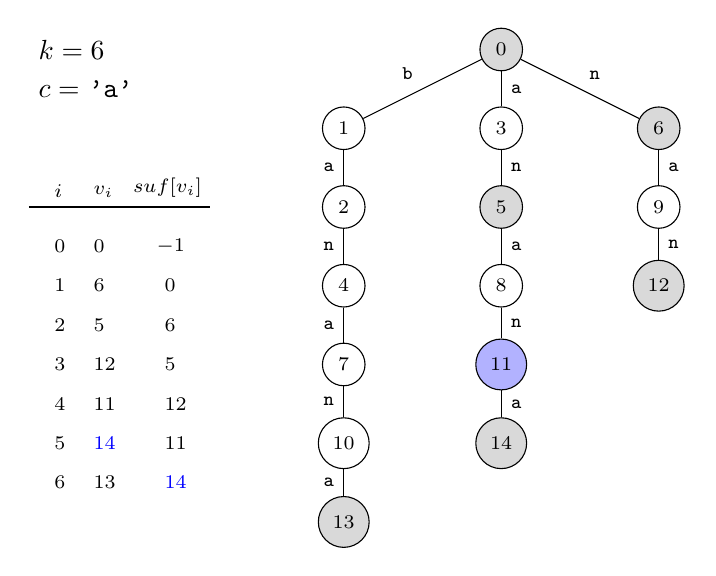
\begin{tikzpicture}
            \node[anchor=west] at (-2, 7) { $k = 6$ };
            \node[anchor=west,opacity=1] at (-2, 6.5) { $c = $ \texttt{'a'} };

            \node[anchor=south west] at (-1.8, 5) { \scriptsize $i$ };
            \node[anchor=south west] at (-1.3, 5) { \scriptsize $v_i$ };
            \node[anchor=south west] at (-0.8, 5) { \scriptsize $suf[v_i]$ };
            \draw[thick] (-2, 5) -- (0.3, 5);

            \node[anchor=west] at (-1.8, 4.5) { \scriptsize $0$ };
            \node[anchor=west] at (-1.3, 4.5) { \scriptsize $0$ };
            \node[anchor=west] at (-0.5, 4.5) { \scriptsize $-1$ };
            
            \node[anchor=west] at (-1.8, 4.0) { \scriptsize $1$ };
            \node[anchor=west] at (-1.3, 4.0) { \scriptsize \textcolor{black}{$6$} };
            \node[anchor=west] at (-0.4, 4.0) { \scriptsize $0$ };

            \node[anchor=west] at (-1.8, 3.5) { \scriptsize $2$ };
            \node[anchor=west] at (-1.3, 3.5) { \scriptsize \textcolor{black}{$5$} };
            \node[anchor=west] at (-0.4, 3.5) { \scriptsize \textcolor{black}{$6$} };

            \node[anchor=west] at (-1.8, 3.0) { \scriptsize $3$ };
            \node[anchor=west] at (-1.3, 3.0) { \scriptsize \textcolor{black}{$12$} };
            \node[anchor=west] at (-0.4, 3.0) { \scriptsize \textcolor{black}{$5$} };

            \node[anchor=west] at (-1.8, 2.5) { \scriptsize $4$ };
            \node[anchor=west] at (-1.3, 2.5) { \scriptsize \textcolor{black}{$11$} };
            \node[anchor=west] at (-0.4, 2.5) { \scriptsize \textcolor{black}{$12$} };

            \node[anchor=west] at (-1.8, 2.0) { \scriptsize $5$ };
            \node[anchor=west] at (-1.3, 2.0) { \scriptsize \textcolor{blue}{$14$} };
            \node[anchor=west] at (-0.4, 2.0) { \scriptsize \textcolor{black}{$11$} };

            \node[anchor=west] at (-1.8, 1.5) { \scriptsize $6$ };
            \node[anchor=west] at (-1.3, 1.5) { \scriptsize $13$ };
            \node[anchor=west] at (-0.4, 1.5) { \scriptsize \textcolor{blue}{$14$} };

            \node[circle,draw,opacity=1,fill=gray!30] (A) at (4, 7) {\scriptsize 0};
            \node[circle,draw,opacity=1] (B1) at (2, 6) {\scriptsize 1};
            \node[circle,draw,opacity=1] (B2) at (4, 6) {\scriptsize 3};
            \node[circle,draw,opacity=1,fill=gray!30] (B3) at (6, 6) {\scriptsize 6};
            \node[circle,draw,opacity=1] (C1) at (2, 5) {\scriptsize 2};
            \node[circle,draw,opacity=1,fill=gray!30] (C2) at (4, 5) {\scriptsize 5};
            \node[circle,draw,opacity=1] (C3) at (6, 5) {\scriptsize 9};
            \node[circle,draw,opacity=1] (D1) at (2, 4) {\scriptsize 4};
            \node[circle,draw,opacity=1] (D2) at (4, 4) {\scriptsize 8};
            \node[circle,draw,opacity=1,fill=gray!30] (D3) at (6, 4) {\scriptsize 12};
            \node[circle,draw,opacity=1] (E1) at (2, 3) {\scriptsize 7};
            \node[circle,draw,opacity=1,fill=blue!30] (E2) at (4, 3) {\scriptsize 11};
            \node[circle,draw,opacity=0] (E3) at (6, 3) {\scriptsize 10};
            \node[circle,draw,opacity=1] (F1) at (2, 2) {\scriptsize 10};
            \node[circle,draw,opacity=1,fill=gray!30] (F2) at (4, 2) {\scriptsize 14};
            \node[circle,draw,opacity=1,fill=gray!30] (G1) at (2, 1) {\scriptsize 13};

            \draw (A) -- node[anchor=south east] { \tt \scriptsize b } (B1);
            \draw (A) -- node[anchor=west] { \tt \scriptsize a } (B2);
            \draw (A) -- node[anchor=south west] { \tt \scriptsize n } (B3);
            \draw (B1) -- node[anchor=east] { \tt \scriptsize a } (C1);
            \draw (B2) -- node[anchor=west] { \tt \scriptsize n } (C2);
            \draw (B3) -- node[anchor=west] { \tt \scriptsize a } (C3);
            \draw (C1) -- node[anchor=east] { \tt \scriptsize n } (D1);
            \draw (C2) -- node[anchor=west] { \tt \scriptsize a } (D2);
            \draw (C3) -- node[anchor=west] { \tt \scriptsize n } (D3);
            \draw (D1) -- node[anchor=east] { \tt \scriptsize a } (E1);
            \draw (D2) -- node[anchor=west] { \tt \scriptsize n } (E2);
%            \draw (D3) -- node[anchor=west] { A } (E3);
            \draw (E1) -- node[anchor=east] { \tt \scriptsize n } (F1);
            \draw (E2) -- node[anchor=west] { \tt \scriptsize a } (F2);
            \draw (F1) -- node[anchor=east] { \tt \scriptsize a } (G1);
%
%            \node[circle] (N1) at (G1) { };
%            \node[circle] (N2) at (F2) { };
%            \node[circle] (N3) at (E3) { };
%            \node[circle] (N4) at (D2) { };
%            \node[circle] (N5) at (C3) { };
%            \node[circle] (N6) at (B2) { };
%
%            \draw[dashed,->] (N1) -- (N2);
%            \draw[dashed,->] (N2) -- (N3);
%            \draw[dashed,->] (N3) -- (N4);
%            \draw[dashed,->] (N4) -- (N5);
%            \draw[dashed,->] (N5) -- (N6);
    \end{tikzpicture}
\end{frame}

\begin{frame}[fragile]{Visualização da construção {\it online} da {\it trie}}

    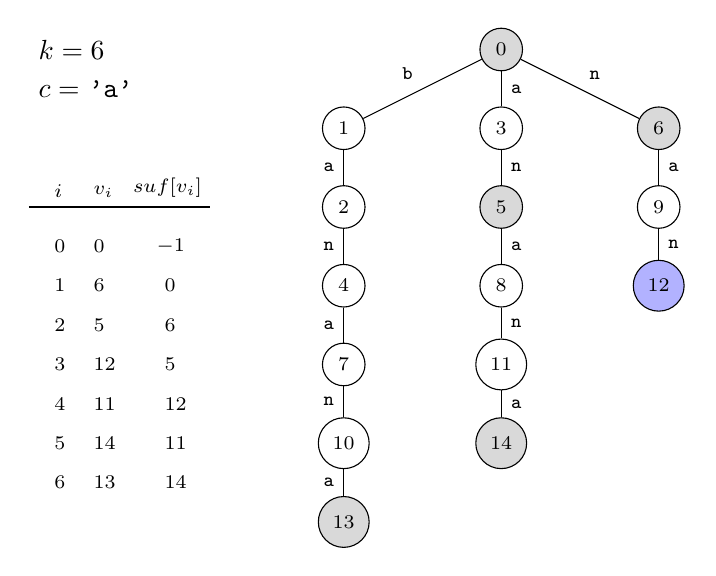
\begin{tikzpicture}
            \node[anchor=west] at (-2, 7) { $k = 6$ };
            \node[anchor=west,opacity=1] at (-2, 6.5) { $c = $ \texttt{'a'} };

            \node[anchor=south west] at (-1.8, 5) { \scriptsize $i$ };
            \node[anchor=south west] at (-1.3, 5) { \scriptsize $v_i$ };
            \node[anchor=south west] at (-0.8, 5) { \scriptsize $suf[v_i]$ };
            \draw[thick] (-2, 5) -- (0.3, 5);

            \node[anchor=west] at (-1.8, 4.5) { \scriptsize $0$ };
            \node[anchor=west] at (-1.3, 4.5) { \scriptsize $0$ };
            \node[anchor=west] at (-0.5, 4.5) { \scriptsize $-1$ };
            
            \node[anchor=west] at (-1.8, 4.0) { \scriptsize $1$ };
            \node[anchor=west] at (-1.3, 4.0) { \scriptsize \textcolor{black}{$6$} };
            \node[anchor=west] at (-0.4, 4.0) { \scriptsize $0$ };

            \node[anchor=west] at (-1.8, 3.5) { \scriptsize $2$ };
            \node[anchor=west] at (-1.3, 3.5) { \scriptsize \textcolor{black}{$5$} };
            \node[anchor=west] at (-0.4, 3.5) { \scriptsize \textcolor{black}{$6$} };

            \node[anchor=west] at (-1.8, 3.0) { \scriptsize $3$ };
            \node[anchor=west] at (-1.3, 3.0) { \scriptsize \textcolor{black}{$12$} };
            \node[anchor=west] at (-0.4, 3.0) { \scriptsize \textcolor{black}{$5$} };

            \node[anchor=west] at (-1.8, 2.5) { \scriptsize $4$ };
            \node[anchor=west] at (-1.3, 2.5) { \scriptsize \textcolor{black}{$11$} };
            \node[anchor=west] at (-0.4, 2.5) { \scriptsize \textcolor{black}{$12$} };

            \node[anchor=west] at (-1.8, 2.0) { \scriptsize $5$ };
            \node[anchor=west] at (-1.3, 2.0) { \scriptsize \textcolor{black}{$14$} };
            \node[anchor=west] at (-0.4, 2.0) { \scriptsize \textcolor{black}{$11$} };

            \node[anchor=west] at (-1.8, 1.5) { \scriptsize $6$ };
            \node[anchor=west] at (-1.3, 1.5) { \scriptsize $13$ };
            \node[anchor=west] at (-0.4, 1.5) { \scriptsize \textcolor{black}{$14$} };

            \node[circle,draw,opacity=1,fill=gray!30] (A) at (4, 7) {\scriptsize 0};
            \node[circle,draw,opacity=1] (B1) at (2, 6) {\scriptsize 1};
            \node[circle,draw,opacity=1] (B2) at (4, 6) {\scriptsize 3};
            \node[circle,draw,opacity=1,fill=gray!30] (B3) at (6, 6) {\scriptsize 6};
            \node[circle,draw,opacity=1] (C1) at (2, 5) {\scriptsize 2};
            \node[circle,draw,opacity=1,fill=gray!30] (C2) at (4, 5) {\scriptsize 5};
            \node[circle,draw,opacity=1] (C3) at (6, 5) {\scriptsize 9};
            \node[circle,draw,opacity=1] (D1) at (2, 4) {\scriptsize 4};
            \node[circle,draw,opacity=1] (D2) at (4, 4) {\scriptsize 8};
            \node[circle,draw,opacity=1,fill=blue!30] (D3) at (6, 4) {\scriptsize 12};
            \node[circle,draw,opacity=1] (E1) at (2, 3) {\scriptsize 7};
            \node[circle,draw,opacity=1] (E2) at (4, 3) {\scriptsize 11};
            \node[circle,draw,opacity=0] (E3) at (6, 3) {\scriptsize 10};
            \node[circle,draw,opacity=1] (F1) at (2, 2) {\scriptsize 10};
            \node[circle,draw,opacity=1,fill=gray!30] (F2) at (4, 2) {\scriptsize 14};
            \node[circle,draw,opacity=1,fill=gray!30] (G1) at (2, 1) {\scriptsize 13};

            \draw (A) -- node[anchor=south east] { \tt \scriptsize b } (B1);
            \draw (A) -- node[anchor=west] { \tt \scriptsize a } (B2);
            \draw (A) -- node[anchor=south west] { \tt \scriptsize n } (B3);
            \draw (B1) -- node[anchor=east] { \tt \scriptsize a } (C1);
            \draw (B2) -- node[anchor=west] { \tt \scriptsize n } (C2);
            \draw (B3) -- node[anchor=west] { \tt \scriptsize a } (C3);
            \draw (C1) -- node[anchor=east] { \tt \scriptsize n } (D1);
            \draw (C2) -- node[anchor=west] { \tt \scriptsize a } (D2);
            \draw (C3) -- node[anchor=west] { \tt \scriptsize n } (D3);
            \draw (D1) -- node[anchor=east] { \tt \scriptsize a } (E1);
            \draw (D2) -- node[anchor=west] { \tt \scriptsize n } (E2);
%            \draw (D3) -- node[anchor=west] { A } (E3);
            \draw (E1) -- node[anchor=east] { \tt \scriptsize n } (F1);
            \draw (E2) -- node[anchor=west] { \tt \scriptsize a } (F2);
            \draw (F1) -- node[anchor=east] { \tt \scriptsize a } (G1);
%
%            \node[circle] (N1) at (G1) { };
%            \node[circle] (N2) at (F2) { };
%            \node[circle] (N3) at (E3) { };
%            \node[circle] (N4) at (D2) { };
%            \node[circle] (N5) at (C3) { };
%            \node[circle] (N6) at (B2) { };
%
%            \draw[dashed,->] (N1) -- (N2);
%            \draw[dashed,->] (N2) -- (N3);
%            \draw[dashed,->] (N3) -- (N4);
%            \draw[dashed,->] (N4) -- (N5);
%            \draw[dashed,->] (N5) -- (N6);
    \end{tikzpicture}
\end{frame}

\begin{frame}[fragile]{Visualização da construção {\it online} da {\it trie}}

    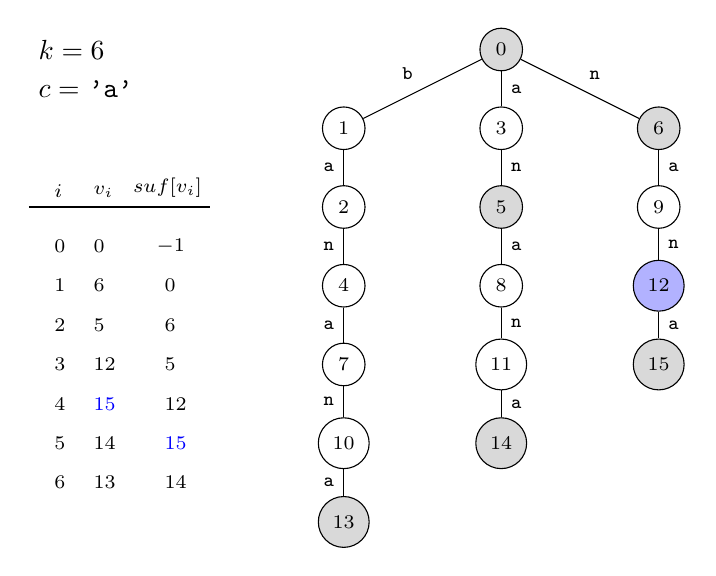
\begin{tikzpicture}
            \node[anchor=west] at (-2, 7) { $k = 6$ };
            \node[anchor=west,opacity=1] at (-2, 6.5) { $c = $ \texttt{'a'} };

            \node[anchor=south west] at (-1.8, 5) { \scriptsize $i$ };
            \node[anchor=south west] at (-1.3, 5) { \scriptsize $v_i$ };
            \node[anchor=south west] at (-0.8, 5) { \scriptsize $suf[v_i]$ };
            \draw[thick] (-2, 5) -- (0.3, 5);

            \node[anchor=west] at (-1.8, 4.5) { \scriptsize $0$ };
            \node[anchor=west] at (-1.3, 4.5) { \scriptsize $0$ };
            \node[anchor=west] at (-0.5, 4.5) { \scriptsize $-1$ };
            
            \node[anchor=west] at (-1.8, 4.0) { \scriptsize $1$ };
            \node[anchor=west] at (-1.3, 4.0) { \scriptsize \textcolor{black}{$6$} };
            \node[anchor=west] at (-0.4, 4.0) { \scriptsize $0$ };

            \node[anchor=west] at (-1.8, 3.5) { \scriptsize $2$ };
            \node[anchor=west] at (-1.3, 3.5) { \scriptsize \textcolor{black}{$5$} };
            \node[anchor=west] at (-0.4, 3.5) { \scriptsize \textcolor{black}{$6$} };

            \node[anchor=west] at (-1.8, 3.0) { \scriptsize $3$ };
            \node[anchor=west] at (-1.3, 3.0) { \scriptsize \textcolor{black}{$12$} };
            \node[anchor=west] at (-0.4, 3.0) { \scriptsize \textcolor{black}{$5$} };

            \node[anchor=west] at (-1.8, 2.5) { \scriptsize $4$ };
            \node[anchor=west] at (-1.3, 2.5) { \scriptsize \textcolor{blue}{$15$} };
            \node[anchor=west] at (-0.4, 2.5) { \scriptsize \textcolor{black}{$12$} };

            \node[anchor=west] at (-1.8, 2.0) { \scriptsize $5$ };
            \node[anchor=west] at (-1.3, 2.0) { \scriptsize \textcolor{black}{$14$} };
            \node[anchor=west] at (-0.4, 2.0) { \scriptsize \textcolor{blue}{$15$} };

            \node[anchor=west] at (-1.8, 1.5) { \scriptsize $6$ };
            \node[anchor=west] at (-1.3, 1.5) { \scriptsize $13$ };
            \node[anchor=west] at (-0.4, 1.5) { \scriptsize \textcolor{black}{$14$} };

            \node[circle,draw,opacity=1,fill=gray!30] (A) at (4, 7) {\scriptsize 0};
            \node[circle,draw,opacity=1] (B1) at (2, 6) {\scriptsize 1};
            \node[circle,draw,opacity=1] (B2) at (4, 6) {\scriptsize 3};
            \node[circle,draw,opacity=1,fill=gray!30] (B3) at (6, 6) {\scriptsize 6};
            \node[circle,draw,opacity=1] (C1) at (2, 5) {\scriptsize 2};
            \node[circle,draw,opacity=1,fill=gray!30] (C2) at (4, 5) {\scriptsize 5};
            \node[circle,draw,opacity=1] (C3) at (6, 5) {\scriptsize 9};
            \node[circle,draw,opacity=1] (D1) at (2, 4) {\scriptsize 4};
            \node[circle,draw,opacity=1] (D2) at (4, 4) {\scriptsize 8};
            \node[circle,draw,opacity=1,fill=blue!30] (D3) at (6, 4) {\scriptsize 12};
            \node[circle,draw,opacity=1] (E1) at (2, 3) {\scriptsize 7};
            \node[circle,draw,opacity=1] (E2) at (4, 3) {\scriptsize 11};
            \node[circle,draw,opacity=1,fill=gray!30] (E3) at (6, 3) {\scriptsize 15};
            \node[circle,draw,opacity=1] (F1) at (2, 2) {\scriptsize 10};
            \node[circle,draw,opacity=1,fill=gray!30] (F2) at (4, 2) {\scriptsize 14};
            \node[circle,draw,opacity=1,fill=gray!30] (G1) at (2, 1) {\scriptsize 13};

            \draw (A) -- node[anchor=south east] { \tt \scriptsize b } (B1);
            \draw (A) -- node[anchor=west] { \tt \scriptsize a } (B2);
            \draw (A) -- node[anchor=south west] { \tt \scriptsize n } (B3);
            \draw (B1) -- node[anchor=east] { \tt \scriptsize a } (C1);
            \draw (B2) -- node[anchor=west] { \tt \scriptsize n } (C2);
            \draw (B3) -- node[anchor=west] { \tt \scriptsize a } (C3);
            \draw (C1) -- node[anchor=east] { \tt \scriptsize n } (D1);
            \draw (C2) -- node[anchor=west] { \tt \scriptsize a } (D2);
            \draw (C3) -- node[anchor=west] { \tt \scriptsize n } (D3);
            \draw (D1) -- node[anchor=east] { \tt \scriptsize a } (E1);
            \draw (D2) -- node[anchor=west] { \tt \scriptsize n } (E2);
            \draw (D3) -- node[anchor=west] { \tt \scriptsize a } (E3);
            \draw (E1) -- node[anchor=east] { \tt \scriptsize n } (F1);
            \draw (E2) -- node[anchor=west] { \tt \scriptsize a } (F2);
            \draw (F1) -- node[anchor=east] { \tt \scriptsize a } (G1);
    \end{tikzpicture}
\end{frame}

\begin{frame}[fragile]{Visualização da construção {\it online} da {\it trie}}

    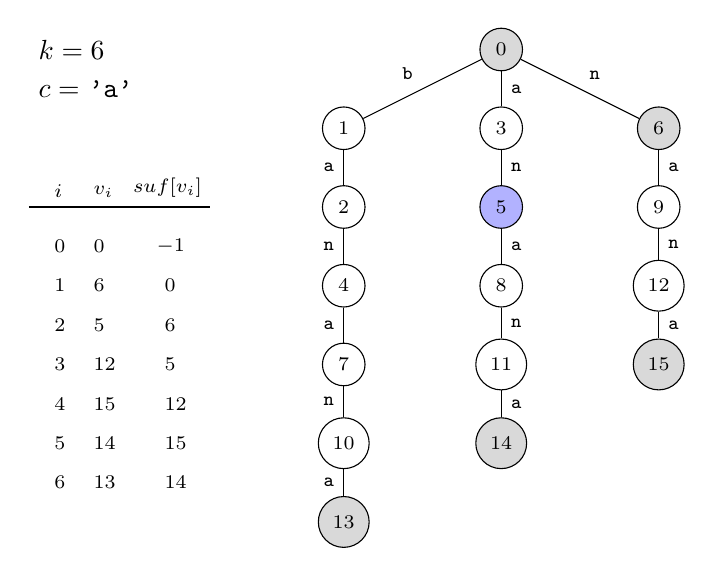
\begin{tikzpicture}
            \node[anchor=west] at (-2, 7) { $k = 6$ };
            \node[anchor=west,opacity=1] at (-2, 6.5) { $c = $ \texttt{'a'} };

            \node[anchor=south west] at (-1.8, 5) { \scriptsize $i$ };
            \node[anchor=south west] at (-1.3, 5) { \scriptsize $v_i$ };
            \node[anchor=south west] at (-0.8, 5) { \scriptsize $suf[v_i]$ };
            \draw[thick] (-2, 5) -- (0.3, 5);

            \node[anchor=west] at (-1.8, 4.5) { \scriptsize $0$ };
            \node[anchor=west] at (-1.3, 4.5) { \scriptsize $0$ };
            \node[anchor=west] at (-0.5, 4.5) { \scriptsize $-1$ };
            
            \node[anchor=west] at (-1.8, 4.0) { \scriptsize $1$ };
            \node[anchor=west] at (-1.3, 4.0) { \scriptsize \textcolor{black}{$6$} };
            \node[anchor=west] at (-0.4, 4.0) { \scriptsize $0$ };

            \node[anchor=west] at (-1.8, 3.5) { \scriptsize $2$ };
            \node[anchor=west] at (-1.3, 3.5) { \scriptsize \textcolor{black}{$5$} };
            \node[anchor=west] at (-0.4, 3.5) { \scriptsize \textcolor{black}{$6$} };

            \node[anchor=west] at (-1.8, 3.0) { \scriptsize $3$ };
            \node[anchor=west] at (-1.3, 3.0) { \scriptsize \textcolor{black}{$12$} };
            \node[anchor=west] at (-0.4, 3.0) { \scriptsize \textcolor{black}{$5$} };

            \node[anchor=west] at (-1.8, 2.5) { \scriptsize $4$ };
            \node[anchor=west] at (-1.3, 2.5) { \scriptsize \textcolor{black}{$15$} };
            \node[anchor=west] at (-0.4, 2.5) { \scriptsize \textcolor{black}{$12$} };

            \node[anchor=west] at (-1.8, 2.0) { \scriptsize $5$ };
            \node[anchor=west] at (-1.3, 2.0) { \scriptsize \textcolor{black}{$14$} };
            \node[anchor=west] at (-0.4, 2.0) { \scriptsize \textcolor{black}{$15$} };

            \node[anchor=west] at (-1.8, 1.5) { \scriptsize $6$ };
            \node[anchor=west] at (-1.3, 1.5) { \scriptsize $13$ };
            \node[anchor=west] at (-0.4, 1.5) { \scriptsize \textcolor{black}{$14$} };

            \node[circle,draw,opacity=1,fill=gray!30] (A) at (4, 7) {\scriptsize 0};
            \node[circle,draw,opacity=1] (B1) at (2, 6) {\scriptsize 1};
            \node[circle,draw,opacity=1] (B2) at (4, 6) {\scriptsize 3};
            \node[circle,draw,opacity=1,fill=gray!30] (B3) at (6, 6) {\scriptsize 6};
            \node[circle,draw,opacity=1] (C1) at (2, 5) {\scriptsize 2};
            \node[circle,draw,opacity=1,fill=blue!30] (C2) at (4, 5) {\scriptsize 5};
            \node[circle,draw,opacity=1] (C3) at (6, 5) {\scriptsize 9};
            \node[circle,draw,opacity=1] (D1) at (2, 4) {\scriptsize 4};
            \node[circle,draw,opacity=1] (D2) at (4, 4) {\scriptsize 8};
            \node[circle,draw,opacity=1] (D3) at (6, 4) {\scriptsize 12};
            \node[circle,draw,opacity=1] (E1) at (2, 3) {\scriptsize 7};
            \node[circle,draw,opacity=1] (E2) at (4, 3) {\scriptsize 11};
            \node[circle,draw,opacity=1,fill=gray!30] (E3) at (6, 3) {\scriptsize 15};
            \node[circle,draw,opacity=1] (F1) at (2, 2) {\scriptsize 10};
            \node[circle,draw,opacity=1,fill=gray!30] (F2) at (4, 2) {\scriptsize 14};
            \node[circle,draw,opacity=1,fill=gray!30] (G1) at (2, 1) {\scriptsize 13};

            \draw (A) -- node[anchor=south east] { \tt \scriptsize b } (B1);
            \draw (A) -- node[anchor=west] { \tt \scriptsize a } (B2);
            \draw (A) -- node[anchor=south west] { \tt \scriptsize n } (B3);
            \draw (B1) -- node[anchor=east] { \tt \scriptsize a } (C1);
            \draw (B2) -- node[anchor=west] { \tt \scriptsize n } (C2);
            \draw (B3) -- node[anchor=west] { \tt \scriptsize a } (C3);
            \draw (C1) -- node[anchor=east] { \tt \scriptsize n } (D1);
            \draw (C2) -- node[anchor=west] { \tt \scriptsize a } (D2);
            \draw (C3) -- node[anchor=west] { \tt \scriptsize n } (D3);
            \draw (D1) -- node[anchor=east] { \tt \scriptsize a } (E1);
            \draw (D2) -- node[anchor=west] { \tt \scriptsize n } (E2);
            \draw (D3) -- node[anchor=west] { \tt \scriptsize a } (E3);
            \draw (E1) -- node[anchor=east] { \tt \scriptsize n } (F1);
            \draw (E2) -- node[anchor=west] { \tt \scriptsize a } (F2);
            \draw (F1) -- node[anchor=east] { \tt \scriptsize a } (G1);
    \end{tikzpicture}
\end{frame}

\begin{frame}[fragile]{Visualização da construção {\it online} da {\it trie}}

    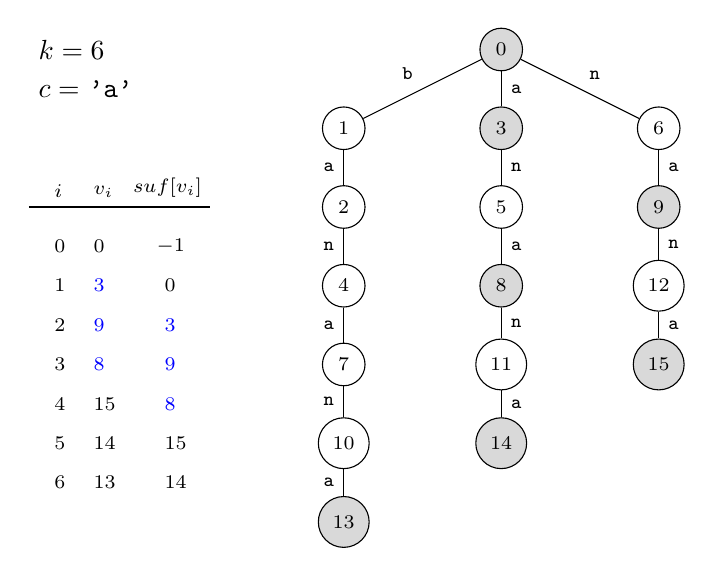
\begin{tikzpicture}
            \node[anchor=west] at (-2, 7) { $k = 6$ };
            \node[anchor=west,opacity=1] at (-2, 6.5) { $c = $ \texttt{'a'} };

            \node[anchor=south west] at (-1.8, 5) { \scriptsize $i$ };
            \node[anchor=south west] at (-1.3, 5) { \scriptsize $v_i$ };
            \node[anchor=south west] at (-0.8, 5) { \scriptsize $suf[v_i]$ };
            \draw[thick] (-2, 5) -- (0.3, 5);

            \node[anchor=west] at (-1.8, 4.5) { \scriptsize $0$ };
            \node[anchor=west] at (-1.3, 4.5) { \scriptsize $0$ };
            \node[anchor=west] at (-0.5, 4.5) { \scriptsize $-1$ };
            
            \node[anchor=west] at (-1.8, 4.0) { \scriptsize $1$ };
            \node[anchor=west] at (-1.3, 4.0) { \scriptsize \textcolor{blue}{$3$} };
            \node[anchor=west] at (-0.4, 4.0) { \scriptsize $0$ };

            \node[anchor=west] at (-1.8, 3.5) { \scriptsize $2$ };
            \node[anchor=west] at (-1.3, 3.5) { \scriptsize \textcolor{blue}{$9$} };
            \node[anchor=west] at (-0.4, 3.5) { \scriptsize \textcolor{blue}{$3$} };

            \node[anchor=west] at (-1.8, 3.0) { \scriptsize $3$ };
            \node[anchor=west] at (-1.3, 3.0) { \scriptsize \textcolor{blue}{$8$} };
            \node[anchor=west] at (-0.4, 3.0) { \scriptsize \textcolor{blue}{$9$} };

            \node[anchor=west] at (-1.8, 2.5) { \scriptsize $4$ };
            \node[anchor=west] at (-1.3, 2.5) { \scriptsize \textcolor{black}{$15$} };
            \node[anchor=west] at (-0.4, 2.5) { \scriptsize \textcolor{blue}{$8$} };

            \node[anchor=west] at (-1.8, 2.0) { \scriptsize $5$ };
            \node[anchor=west] at (-1.3, 2.0) { \scriptsize \textcolor{black}{$14$} };
            \node[anchor=west] at (-0.4, 2.0) { \scriptsize \textcolor{black}{$15$} };

            \node[anchor=west] at (-1.8, 1.5) { \scriptsize $6$ };
            \node[anchor=west] at (-1.3, 1.5) { \scriptsize $13$ };
            \node[anchor=west] at (-0.4, 1.5) { \scriptsize \textcolor{black}{$14$} };

            \node[circle,draw,opacity=1,fill=gray!30] (A) at (4, 7) {\scriptsize 0};
            \node[circle,draw,opacity=1] (B1) at (2, 6) {\scriptsize 1};
            \node[circle,draw,opacity=1,fill=gray!30] (B2) at (4, 6) {\scriptsize 3};
            \node[circle,draw,opacity=1] (B3) at (6, 6) {\scriptsize 6};
            \node[circle,draw,opacity=1] (C1) at (2, 5) {\scriptsize 2};
            \node[circle,draw,opacity=1] (C2) at (4, 5) {\scriptsize 5};
            \node[circle,draw,opacity=1,fill=gray!30] (C3) at (6, 5) {\scriptsize 9};
            \node[circle,draw,opacity=1] (D1) at (2, 4) {\scriptsize 4};
            \node[circle,draw,opacity=1,fill=gray!30] (D2) at (4, 4) {\scriptsize 8};
            \node[circle,draw,opacity=1] (D3) at (6, 4) {\scriptsize 12};
            \node[circle,draw,opacity=1] (E1) at (2, 3) {\scriptsize 7};
            \node[circle,draw,opacity=1] (E2) at (4, 3) {\scriptsize 11};
            \node[circle,draw,opacity=1,fill=gray!30] (E3) at (6, 3) {\scriptsize 15};
            \node[circle,draw,opacity=1] (F1) at (2, 2) {\scriptsize 10};
            \node[circle,draw,opacity=1,fill=gray!30] (F2) at (4, 2) {\scriptsize 14};
            \node[circle,draw,opacity=1,fill=gray!30] (G1) at (2, 1) {\scriptsize 13};

            \draw (A) -- node[anchor=south east] { \tt \scriptsize b } (B1);
            \draw (A) -- node[anchor=west] { \tt \scriptsize a } (B2);
            \draw (A) -- node[anchor=south west] { \tt \scriptsize n } (B3);
            \draw (B1) -- node[anchor=east] { \tt \scriptsize a } (C1);
            \draw (B2) -- node[anchor=west] { \tt \scriptsize n } (C2);
            \draw (B3) -- node[anchor=west] { \tt \scriptsize a } (C3);
            \draw (C1) -- node[anchor=east] { \tt \scriptsize n } (D1);
            \draw (C2) -- node[anchor=west] { \tt \scriptsize a } (D2);
            \draw (C3) -- node[anchor=west] { \tt \scriptsize n } (D3);
            \draw (D1) -- node[anchor=east] { \tt \scriptsize a } (E1);
            \draw (D2) -- node[anchor=west] { \tt \scriptsize n } (E2);
            \draw (D3) -- node[anchor=west] { \tt \scriptsize a } (E3);
            \draw (E1) -- node[anchor=east] { \tt \scriptsize n } (F1);
            \draw (E2) -- node[anchor=west] { \tt \scriptsize a } (F2);
            \draw (F1) -- node[anchor=east] { \tt \scriptsize a } (G1);
    \end{tikzpicture}
\end{frame}

